\documentclass[12pt,a4paper]{book}

\usepackage{epsfig}
\usepackage{graphicx}
\usepackage{graphics}
\usepackage{color}
\usepackage{algorithm}
\usepackage{algorithmic}
\usepackage[portuges]{babel}
\usepackage{fancyhdr}

\newcommand{\ds}[1]{\mbox{$\displaystyle  #1 $}}
\renewcommand{\algorithmicrequire}{\textbf{Entrada:}}
\renewcommand{\algorithmicensure}{\textbf{Saida:}}
\renewcommand{\algorithmicend}{\textbf{fim}}
\renewcommand{\algorithmicif}{\textbf{Se}}
\renewcommand{\algorithmicelse}{\textbf{sen\~{a}o}}
\renewcommand{\algorithmicdo}{\textbf{fa\c{c}a}}
\renewcommand{\algorithmicwhile}{\textbf{enquanto}}
\renewcommand{\algorithmicfor}{\textbf{para}}
\renewcommand{\algorithmicthen}{\textbf{ent\~{a}o}}
\floatname{algorithm}{Algoritmo}

\newtheorem{Def}{Defini\c{c}\~{a}o}
\newtheorem{Lem}{Lema}
\newtheorem{Teo}{Teorema}
\newtheorem{Cor}{Corol\'ario}

%passa a imprimir a partir do canto superior esquerdo do papel
%respeitando os atributos de diagramacao selecionados
%dvips -t A4 -O -2.54cm,-2.54cm filename

\textwidth = 14cm
\textheight 44\baselineskip
\hoffset -1in
\voffset -4pt
\headsep = 29pt
\topmargin = 0pt
\oddsidemargin 3.5cm
\evensidemargin 3.5cm
\frenchspacing
\sloppy

\begin{document}

\input rotate
\newbox\rotbox
\newbox\rottwo
\bibliographystyle{acm}
%\bibliographystyle{plain}


\pagestyle{fancy}
\renewcommand{\headrulewidth}{0.pt}
\pagenumbering{roman}

\fancyhead{}   %clear all fields
\fancyfoot[OC,EC]{}

\newpage

\thispagestyle{empty}

\begin{figure}[htbp]
  \leavevmode
  %\epsfig{file = Unesp-1.eps, height = 2cm, width = 3.95cm}
  
\includegraphics[scale = 0.4]{PaginasIniciais/unesplogo.eps}
\end{figure}

\hspace{15mm}
\vspace{23mm}
\begin{minipage}{155mm}
\vskip-30mm
\begin{center}
\Large UNIVERSIDADE ESTADUAL PAULISTA \\ ``J\'{U}LIO DE MESQUITA FILHO" \\[2mm]
\normalsize  C\^{a}mpus de Presidente Prudente 
\end{center}
\end{minipage}

%\vspace{10mm}

%\vspace{60mm}

%\hspace*{-5mm}
\vspace{-15mm}

\begin{center}
\Large  {\bf Triangula\c{c}\~{a}o de Delaunay no Plano: Algoritmos de Inser\c{c}\~{a}o}
\end{center}
\vspace{10mm}
\begin{figure}[htbp]
  \begin{center}
    \leavevmode
    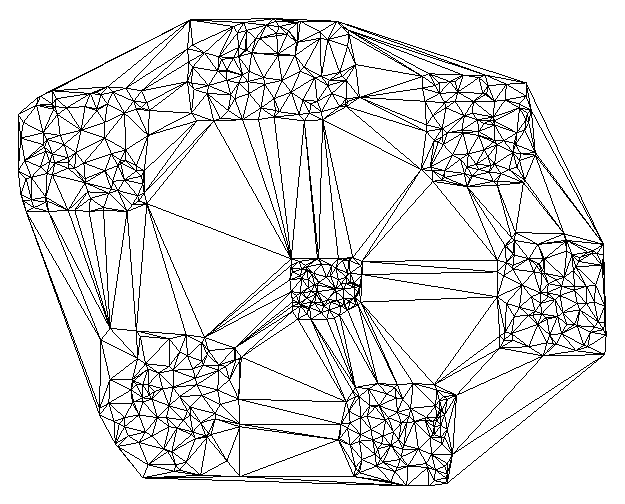
\epsfig{file = PaginasIniciais/fig_capa.eps,height=8cm, width=8cm}
 \end{center}
\end{figure}
\vspace{2mm}
\begin{center}
\large {\bf Anderson Greg\'orio da Silva}\\
\normalsize Monografia para Conclus\~{a}o de Curso \\[5mm]
%\vspace{mm}
\large {\bf Orientador: Marco Ant\^{o}nio Piteri }\\
\vspace{26mm}
%\vspace{4mm}
%Documento Provis\'{o}rio
\large \bf PRESIDENTE PRUDENTE \\ JANEIRO DE 2008
\end{center}


%\thispagestyle{empty}
%\phantom{text}

\hspace{-5mm}{\Large {\bf  }}  \\ [6mm]



\thispagestyle{empty}
\vspace{20mm}

\begin{center}
\large \bf{ANDERSON GREG\'ORIO DA SILVA}

\vspace{80mm}

\large \bf{TRIANGULA\c{C}\~{A}O DE DELAUNAY NO PLANO: ALGORITMOS DE INSER\c{C}\~{A}O}
\end{center}
\vspace{5mm}
\hspace{50mm}
\begin{minipage}{100mm}
Monografia apresentada ao curso de Bacharelado em Ci\^{e}ncia da Computa\c{c}\~{a}o da Faculdade de Ci\^{e}ncias e Tecnologia/UNESP - C\^{a}mpus de Presidente Prudente, como requisito para a conclus\~{a}o do curso.
\end{minipage}
\vspace{80mm}
\begin{center}
\textbf{PRESIDENTE PRUDENTE \\ 2008} 
\end{center}
\newpage
\hspace{-5mm}{\Large {\bf  }}  \\ [6mm]



\thispagestyle{empty}
\vspace{20mm}
\begin{center}
\Large \bf{TERMO APROVA\c{C}\~{A}O}\\
\vspace{50mm}
\large ANDERSON GREG\'ORIO DA SILVA\\
\vspace{25mm}
\large TRIANGULA\c{C}\~{A}O DE DELAUNAY NO PLANO: ALGORITMOS DE INSER\c{C}\~{A}O \\
\normalsize
\end{center}
\vspace{15mm}
\begin{minipage}{150mm}
 Monografia aprovada como requisito parcial para conclus\~{a}o do curso de Bacharelado em C\^{i}encia da Computa\c{c}\~{a}o, da Faculdade de C\^{i}encia e Tecnologia/UNESP, pela seguinte banca examinadora:\\
\end{minipage}
\begin{minipage}{150mm}
\vspace{10mm}

Orientador: \hspace{3mm} Prof. Dr. Marco Ant\^{o}nio Piteri

\hspace{25mm} Departamento de Matem\'{a}tica, Estat\'{i}stica e Computa\c{c}\~{a}o - UNESP \\ \\

\hspace{25mm} Prof. Dr. Ronado Celso Messias

\hspace{25mm} Departamento de Matem\'{a}tica, Estat\'{i}stica e Computa\c{c}\~{a}o - UNESP \\ \\

\hspace{25mm} Prof. Dr. Messias Meneguetti Junior

\hspace{25mm} Departamento de Matem\'{a}tica, Estat\'{i}stica e Computa\c{c}\~{a}o - UNESP \\ \\
\end{minipage}
\vspace{12mm}
\begin{center}
Presidente Prudente, 30 de Janeiro de 2008
\end{center}




\hspace{-5mm}{\Large {\bf  }}  \\ [6mm]




\fancyhead{}   %clear all fields
\fancyfoot[OC,EC]{\vspace{3mm}\bfseries\thepage}
\fancyhead[EL]{}
\fancyhead[EC]{}
\fancyhead[ER]{\sc \leftmark}
\fancyhead[OL]{}
\fancyhead[OC]{}
\fancyhead[OR]{}

\setcounter{page}{5}
\hspace{-5mm}{\Large {\bf Agradecimentos }}  \\ [6mm]

A realiza\c{c}\~{a}o do presente curso foi poss\'ivel devido \`a colabora\c{c}\~{a}o de muitas pessoas que me auxiliaram durante os 5 anos de curso. Manifesto assim minha gratid\~ao:
\\

 primeiramente a Deus, que sempre me ajudou a n\~ao desistir dessa longa caminhada, e que sempre me acompanha durante a execu\c{c}\~{a}o de minhas tarefas. 
\\

%%% Local Variables: 
%%% mode: latex
%%% TeX-master: "tese"
%%% End: 



\hspace{-5mm}{\Large {\bf  }}  \\ [6mm]




\hspace{-7mm}{\Large{\bf Resumo }} \\ [6mm]

Esse trabalho apresenta uma discuss\~ao te\'orica e os resultados obtidos a partir da implementa\c{c}\~ao de algoritmos de inser\c{c}\~ao aplicados ao problema de triangula\c{c}\~ao de Delaunay no plano. A representa\c{c}\~ao de todas as fases do processo construtivo  \'e baseada na estrutura de dados topol\'ogica \textit{winged edge modificada}. Dentre todas as triangula\c{c}\~oes existentes e associadas a um mesmo conjunto de pontos, a triangula\c{c}\~ao de Delaunay \'e aquela que n\~ao s\'o maximiza o menor dos \^angulos, mas garante sob certas condi\c{c}\~oes, a unicidade da triangula\c{c}\~ao. Nesse sentido, a triangula\c{c}\~ao de Delaunay associada a um conjunto de pontos em $R^2$, apresenta caracter\'isticas de regularidade local e global, raz\~ao pela qual \'e indispens\'avel para um amplo conjunto de aplica\c{c}\~oes, como por exemplo, modelagem digital de terrenos e gera\c{c}\~ao autom\'atica de malhas de elementos finitos.

Os resultados previamente obtidos serviram como ponto de partida para que um projeto associado ao diagrama de Voronoi, que \'e o dual da triangulação de Delaunay, pudesse ser obtido de maneira indireta.

\vspace{15mm}

\hspace{-7mm}{\Large {\bf Palavras-Chave:}}\\

\hspace{-7mm}
Triangula\c{c}\~{a}o de Delaunay \\ [2mm]
Estruturas de dados topol\'{o}gicas \\ [2mm]
\textit{winged-edge modificada} \\ [2mm]





%%% Local Variables: 
%%% mode: latex
%%% TeX-master: "tese"
%%% End: 

\hspace{-5mm}{\Large {\bf  }}  \\ [6mm]




\hspace{-7mm}{\Large{\bf Abstract }} \\ [6mm]

That work presents a theoretical discussion and the results obtained from the implementation of insert algorithms applied to the Delaunay triangulation problem in the plane. The representation of all of the phases of the constructive process is based on the \textit{modified winged edge} topological data structure.
 
Among all of the existent triangulations and associated to a same set of points, the Delaunay triangulation is that not only maximizes the smallest of the angles (MaxMin Criterium), but it guarantees under certain conditions, the unicity of the triangulation. In that sense, the triangulation of Delaunay associated to a set of points in $R^2$, presents characteristics of local and global regularity, reason for the which is indispensable for a wide group of applications, as for instance, terrain digital modelling and automatic finite elements meshes generation. The results previously obtained served as starting point so that a project associated to the diagram of Voronoi, that is the dual of the Delaunay triangulation, it could be obtained in an indirect way.


\vspace{15mm}

\hspace{-7mm}{\Large {\bf Keywords}}\\

\hspace{-7mm}
Delaunay Triangulation \\ [2mm]
Topological data structures \\ [2mm]
\textit{modified winged-edge} \\ [2mm]


 
%%% Local Variables: 
%%% mode: latex
%%% TeX-master: "tese"
%%% End: 

\hspace{-5mm}{\Large {\bf  }}  \\ [6mm]



%\hspace{-7mm}{\Large{\bf Nota\c{c}\~{a}o}}

\begin{center}
\begin{tabular}{p{3.0cm}p{10.5cm}}
\multicolumn{2}{l}{\Large{\bf Nota\c{c}\~{a}o}} \\ \\ \\
$\det(A)$ & determinante correspondente \`{a} matriz $A$;\\
$(x,y)$ & par ordenado de pontos  do espa\c{c}o euclideano 2D; \\
${\mathbf G}(V, E)$ & grafo $\mathbf{G}$ com conjunto
de v\'{e}rtices $V$ e arestas $E$; \\ 
$R^{n}$ & espa\c{c}o euclideano de dimens\~{a}o $n$; \\
$P$ & conjunto finito de pontos no espa\c{c}o euclideano de
dimens\~{a}o $ R^n$;\\ 
${\mathbf {p}}_{ix}$ & abscissa do ponto ${\mathbf {p}}_i$; \\
${\mathbf {p}}_{iy}$ & ordenada do ponto ${\mathbf {p}}_i$; \\
$Conv(P)$ & fecho convexo do conjunto $P$; \\
$\Delta({\bf{p}}_{i},{\bf{p}}_{j},{\bf{p}}_{k})$ & triangulo formado pelos 
pontos ${\mathbf{p}}_{i},{\mathbf{p}}_{j}$ e ${\mathbf{p}}_{k}$; \\
$Area({\mathbf{p}}_{i},{\mathbf{p}}_{j},{\mathbf{p}}_{k})$ & \'{a}rea orientada 
do $\Delta({\mathbf{p}}_{i},{\mathbf{p}}_{j},{\mathbf{p}}_{k})$;\\
$\mathit{dist(\mathbf{q}, \mathbf{p})}$ & dist\^{a}ncia euclideana entre os pontos
${\bf p}$ e ${\bf q}$; \\ 
$\overline{{\bf ab}}$ & segmento definido pelos pontos ${\bf a}$ e
${\bf b}$;\\
${V}(P)$ & Diagrama de Voronoi associada ao conjunto de pontos $P$; \\ 
${V}({\mathbf{p}}_{i})$ & regi\~{a}o de Voronoi associada ao ponto ${\mathbf {p}}_{i}$; \\ 
${D}(P)$ & Triangula\c{c}\~{a}o de Delaunay associada ao conjunto de pontos $P$;\\
$\Gamma$ & Representa\c{c}\~{a}o do Parabol\'oide no espa\c{c}o euclidiano $R^3$.\\
\end{tabular}
\end{center}



%%% Local Variables: 
%%% mode: latex
%%% TeX-master: "tese"
%%% End:

\hspace{-5mm}{\Large {\bf  }}  \\ [6mm]




\renewcommand{\headrulewidth}{0.6pt}
\renewcommand{\footrulewidth}{0pt}
\renewcommand{\chaptermark}[1]{\markboth{#1}{}}
\renewcommand{\sectionmark}[1]{\markright{#1}}

\fancyhead{}   %clear all fields
\fancyfoot[OC,EC]{\vspace{3mm}\bfseries\thepage}
\fancyhead[EL]{}
\fancyhead[EC]{}
\fancyhead[ER]{\sc \leftmark}
\fancyhead[OL]{\sc \leftmark}
\fancyhead[OC]{}
\fancyhead[OR]{}


\tableofcontents

\vskip 1.0em plus 1pt  
{\bf Bibliografia \hfill \pageref{pagbib}}
%\listoftables
\listoffigures

\setlength{\parskip}{1em}
\newpage

\fancyhead{}   %clear all fields
\fancyhead[EL]{\sc Cap\'{\i}tulo \thechapter}
\fancyhead[EC]{}
\fancyhead[ER]{\sc \leftmark}
\fancyhead[OL]{\sc \rightmark}
\fancyhead[OC]{}
\fancyhead[OR]{\sc Se\c{c}\~{a}o \thesection}

\newpage
\pagenumbering{arabic}

\chapter{Introdu\c{c}\~{a}o}

\chapter{exemplo}

Essa monografia apresenta uma fundamenta\c{c}\~{a}o te\'orica e os resultados pr\'aticos obtidos segundo a proposta inicial presente no ante-projeto de pesquisa elaborado no in\'icio do ano de 2007.

O projeto aborda um tema cl\'assico na \'area de geometria computacional e consiste no estudo e implementa\c{c}\~ao de t\'ecnicas algor\'itmicas para resolu\c{c}\~{a}o de problemas de natureza geom\'etrica e topol\'ogica. No
escopo da \'area de geometria computacional trabalhamos especificamente na resolu\c{c}\~{a}o de problemas associados a subdivis\~oes planares, mais especialmente aquelas em que todas as regi\~oes s\~ao triangulares. Esse problema tamb\'em \'e conhecido por \textit{triangula\c{c}\~{a}o}.

Do ponto de vista te\'orico o problema de triangula\c{c}\~ao pode ser tratado em muitas dimens\~oes, por\'em suas aplica\c{c}\~{o}es mais imediatas est\~ao restritas  ao espa\c{c}o euclidiano de dimens\~ao 2 e 3. A import\^ancia do assunto \'e tanta que existe uma gama significativa de problemas que podemos citar em que a representa\c{c}\~{a}o de um objeto 2D ou 3D se mostra de suma import\^ancia para melhor visualiza\c{c}\~{a}o ou at\'e mesmo para resolu\c{c}\~{a}o do problema em si, por exemplo, a representa\c{c}\~{a}o prim\'aria de um objeto dado um conjunto finito de pontos obtidos por amostragem, atrav\'es de imagens de sat\'elite, resson\^ancia magn\'etica, ultra-sonografia ou por meio de um mecanismo de leitura autom\'atico, como por exemplo, um scanner 3D gera um subconjunto de ordem 3 e d\'a origem a um conjunto de tri\^angulos que ir\'a aproximar a superf\'icie do objeto que est\'a sendo modelado. Existem outras aplica\c{c}\~{o}es que envolvem o esquema de triangula\c{c}\~{a}o, em que o problema de triangula\c{c}\~{a}o aparece somente como um subproblema a ser resolvido, s\~ao eles:

\begin{description}

\item[1] Vis\~ao por computador/Rob\'otica;
\item[2] Reconstru\c{c}\~{a}o de Curvas e Superf\'icies (modelagem digital de terreno, arqueologia, medicina);
\item[3] Reconstru\c{c}\~{a}o de objetos tridimensionais a partir de se\c{c}\~{o}es transversais;
\item[4] Visualiza\c{c}\~{a}o de superf\'icies matem\'aticas;
\item[5] Gera\c{c}\~{a}o de malhas de elementos finitos.

\end{description}

\section{Organiza\c{c}\~{a}o do Trabalho}

O cap\'itulo \ref{chapter2} cont\'em toda a fundamenta\c{c}\~{a}o te\'orica necess\'aria para entender as t\'ecnicas algor\'itmicas que foram usadas para viabilizar as etapas 
relativas as diferentes implementa\c{c}\~{o}es realizadas. Discute sobre as primitivas geom\'etricas, a estrutura de dados topol\'ogica e os operadores de Euler que foram implementados por meio de operadores topol\'ogicos.

\chapter{Fundamenta\c{c}\~{a}o Te\'orica} \label{chapter2}

\section{Triangula\c{c}\~{a}o}

Antes de iniciarmos ativamente os estudos sobre a estrutura de dados e as primitivas que utilizamos nas nossas implementa\c{c}\~{o}es daremos uma introdu\c{c}\~{a}o b\'asica sobre o que seria uma triangula\c{c}\~{a}o, sua import\^ancia, os diversos tipos e sobre que tipo de dados aplicamos nossos algoritmos.

Triangula\c{c}\~{a}o \'e um problema fundamental em geometria computacional, pois o primeiro passo para se trabalhar com objetos geom\'etricos complexos \'e fazer a decomposi\c{c}\~{a}o em objetos mais simples, o objeto geom\'etrico mais simples que conhecemos no plano \'e o tri\^angulo e no espa\c{c}o o tetraedro. Algumas aplica\c{c}\~{o}es cl\'assicas conhecidas que utilizam triangula\c{c}\~{a}o podem ser, por exemplo, an\'alise de elementos finitos e computa\c{c}\~{a}o gr\'afica. Uma triangula\c{c}\~{a}o tamb\'em pode ser referenciada na literatura como uma \textit{malha de elementos finitos} \cite{piteri1} ou \textit{malha de elementos triangulares}.

Quando trabalhamos no plano, geralmente utilizamos um conjunto de pontos dado como entrada, tais pontos podem ser obtidos por meio de um escaneamento feito em uma superficie planar. Por\'em, quando realizamos isso geralmente h\'a ocorr\^encia de pontos diferentes com mesma coordenada, e o ideal \'e termos pontos \'unicos dados no plano, para isso o que geralmente se faz \'e uma permuta\c{c}\~{a}o entre os dados de entrada, e isso faz com que a ordem de processamento dos pontos n\~ao seja a mesma ordem do scan, esse princ\'ipio denotaremos por \textit{randomiza\c{c}\~{a}o}\cite{guibas}, permitindo que a probabilidade de termos dois pontos de mesma coordenada diminua.

Uma triangula\c{c}\~{a}o pode ser entendida como liga\c{c}\~{a}o de cada ponto do conjunto atrav\'es de uma aresta (tamb\'em denotado como {\bf corda}) formando um tri\^angulo. Existir\~ao arestas que ser\~ao compartilhados por dois tri\^angulos, a triangula\c{c}\~{a}o ocorre quando todos os pontos constituem os \textit{v\'ertices} dos tri\^angulos formados. 

Um problema geom\'etrico interessante \'e o \textit{Fecho Convexo}, trata-se do menor conjunto convexo que cont\'em todos os pontos do conjunto dado, ver figura \ref{relacionamento} representado por linhas s\'olidas mais espessas. \'E importante mencion\'a-lo pois ele cont\'em todos os pontos de um conjunto de pontos j\'a triangularizados, existem diversos algoritmos capazes de comput\'a-lo, mas se conseguirmos a triangula\c{c}\~{a}o do conjunto automaticamentes obteremos o \textit{Fecho Convexo} relativo \`aquele conjunto de pontos.

A triangula\c{c}\~{a}o de um conjunto de pontos n\~ao possui unicidade. Em outras palavras, a partir de um mesmo conjunto de pontos \'e poss\'ivel obter diferentes triangula\c{c}\~{o}es cada uma delas com $2(n-1)k$ tri\^angulos e $3(n-1)-k$ arestas, onde $k$ \'e o n\'umero de pontos pertencentes ao (\textit{Fecho Convexo}) da triangula\c{c}\~{a}o. No caso a forma dos tri\^angulos tamb\'em podem influenciar na aplica\c{c}\~{a}o que se deseja fazer, \'e necess\'ario evitar tri\^angulos muito finos(\^angulos internos muito agudos) na triangula\c{c}\~{a}o como na figura \ref{triangulations} a) e b), o ideal \'e termos tri\^angulos o mais pr\'oximo poss\'ivel dos tri\^angulos equil\'ateros com os \^angulos se aproximando de $60^{\textrm{o}}$, figura \ref{triangulations} c).

\begin{figure}[htbp]
  \begin{center}
    \leavevmode
    \input{Figuras/Chapter2/Triangulations.pstex_t}
    \caption{Poss\'iveis triangula\c{c}\~{o}es para um mesmo conjunto de pontos.}
    \label{triangulations}
  \end{center}
\end{figure}

Foi provado que quando um quarto ponto se encontra no exterior do c\'irculo definido por tr\^es pontos, significa que os \^angulos internos do tri\^angulo que definiu esse c\'irculo ser\~ao os m\'aximos que podem ser obtidos para esse elemento na triangula\c{c}\~{a}o, se todos os elementos da triangula\c{c}\~{a}o obedecerem essa propriedade significa que \'e a melhor triangula\c{c}\~{a}o para aquele conjunto de pontos dado como entrada, essa triangula\c{c}\~{a}o especial \'e \'unica sob certas condi\c{c}\~{o}es, e recebeu o nome de \textit{Triangula\c{c}\~{a}o de Delaunay} figura \ref{relacionamento} representado por linhas s\'olidas mais finas. Falaremos de suas propriedades, rela\c{c}\~{o}es e casos degenerados no cap\'itulo \ref{chapter3}.
 
O Diagrama de Voronoi \'e outro problema geom\'etrico que mencionaremos durante a descri\c{c}\~{a}o, este por sua vez tem rela\c{c}\~{a}o direta com a triangula\c{c}\~{a}o de Delaunay, figura \ref{relacionamento} representado por linhas tracejadas, pois \'e o dual da triangula\c{c}\~{a}o, foi observando esse diagrama que Delaunay obteve sua triangula\c{c}\~{a}o e a rela\c{c}\~{a}o entre os dois problemas geom\'etricos, se conseguir resolver um dos problemas o outro poder\'a ser obtido de maneira indireta. Explicaremos mais detalhadamente as rela\c{c}\~{o}es no cap\'itulo \ref{chapter3}.

\begin{figure}[htbp]
  \begin{center}
    \leavevmode
    \input{Figuras/Chapter2/Relacionamento.pstex_t}
    \caption{Relacionamento entre a \textit{Triangula\c{c}\~{a}o de Delaunay}, o \textit{Diagrama de Voronoi} e o \textit{Fecho Convexo} para um mesmo conjunto de pontos. A \'area hachurada mais clara trata-se de uma regi\~ao de Voronoi, e a \'area hachurada mais escura \'e um tri\^angulo de Delaunay.}
    \label{relacionamento}
  \end{center}
\end{figure}

\section{Primitivas Geom\'{e}tricas}

Nessa pequena introdu\c{c}\~{a}o falaremos sobre a import\^{a}ncia das
primitivas geom\'{e}tricas numa triangula\c{c}\~{a}o e denotaremos algumas
propriedades relevantes.

Pontos cocirculares e pol\'{\i}gonos inscritos possuem muitas propriedades
especiais que permitem uma constru\c{c}\~{a}o eficiente de uma triangula\c{c}%
\~{a}o equiangular \cite{sibson}. Algumas dessas propriedades ser\~{a}o descritas a partir
dos \textit{LEMAS}.

Suponhamos que temos $n$ pontos cocirculares, ligados por $n$ \textit{arestas}
para construir um pol\'{\i}gono convexo inscrito. As $n$ \textit{arestas} s%
\~{a}o cordas do c\'{\i}rculo inscrito, e chamaremos estas de \textbf{cordas
exteriores}. Os demais segmentos entre os pares dos $n$ pontos s\~{a}o as 
\textbf{cordas interiores}. Uma corda interior que omite exatamente um \textit{%
v\'{e}rtice}, ligando o \textit{v\'{e}rtice} $i$ ao $(i+2)$ de $n$ \'{e}
chamada de \textbf{corda intermedi\'{a}ria}. Uma observa\c{c}\~{a}o trivial,
mas vale ressaltar, \'{e} que qualquer triangula\c{c}\~{a}o deve conter no m%
\'{\i}nimo duas \textbf{cordas intermedi\'{a}rias}.

Um \^{a}ngulo est\'{a} inscrito no c\'{\i}rculo se o \textit{v\'{e}rtice}
pertencer ao c\'{\i}rculo e os dois raios interseseccionam o c\'{\i}rculo.
Cada \^{a}ngulo de cada tri\^{a}ngulo da triangula\c{c}\~{a}o cocirculares 
\'{e} um \^{a}ngulo inscrito. Um fato geometricamente cl\'{a}ssico \'{e} que
para um \^{a}ngulo inscrito no c\'{\i}rculo o arco sob o \^{a}ngulo \'{e}
duas vezes maior que o grau angular. Portanto todos os \^{a}ngulos inscritos
subtendidos sobre o mesmo arco tem o mesmo tamanho.

Em qualquer tri{a}ngula\c{c}\~{a}o de um \textit{pol\'igono} de $n$ lados inscrito num c\'{\i}%
rculo, as \textbf{cordas exteriores} s\~{a}o as \textit{arestas} daquela
triangula\c{c}\~{a}o. Cada \textbf{corda exterior} aparece num tri\^{a}ngulo
simples e para esse tri\^{a}ngulo, o \^{a}ngulo oposto \`{a} \textit{aresta}
exterior \'{e} sempre igual \`{a} metade do arco do lado de fora da \textit{%
aresta}. Devido essa raz\~{a}o temos:

\begin{Lem}
: Cada triangula\c{c}\~{a}o de um \textit{pol\'igono} de $n$ lados inscrito ter\'{a} entre seus \^{a}ngulos o mesmo conjunto de $n$ \^{a}ngulos, isto \'{e}, os $n$ \^{a}ngulos opostos \`{a}s $n$ cordas do lado de fora.
\end{Lem}

Cada \textbf{corda interior} de uma tri{a}ngula\c{c}\~{a}o de um \textit{pol\'igono}
de $n$ lados inscrito pertencer\'{a} a dois tri\^{a}ngulos, e os tamanhos dos dois \^{a}ngulos opostos \`{a}s cordas nos dois tri\^{a}ngulos s\~{a}o determinados pelo comprimento da corda e n\~{a}o pela triangula\c{c}\~{a}o em si. Isto \'{e}, os dois \^{a}ngulos s\~{a}o suplementares (soma igual a $180%
%TCIMACRO{\U{b0}}%
%BeginExpansion
{{}^\circ}%
%EndExpansion
$) e cada um equivale \`{a} metade do arco correspondente subtendido pela
corda (um arco maior, um arco menor).

Visto que todos \^{a}ngulos da triangula\c{c}\~{a}o do \textit{pol\'igono} de $n$ lados inscrito
(exceto os \textit{n-conjuntos} ligados associados com as cordas exteriores) s\~{a}%
o dados em pares de suplementares, um acut\^{a}ngulo e outro obtus\^{a}%
ngulo, para maximizar lexicograficamente os acut\^{a}ngulos da triangula\c{c}%
\~{a}o \'{e} necess\'{a}rio maximizar todos os \^{a}ngulos. Mas desde que os
acut\^{a}ngulos para as cordas interiores forem ordenados de acordo com o
comprimento da corda. Temos entao:

\begin{Lem}
: Uma triangula\c{c}\~{a}o de um \textit{pol\'igono} de $n$ lados inscrito ter\'{a} maximiza\c{c}%
\~{a}o lexicograficamente dos \^{a}ngulos dispostos em sequ\^{e}ncia
crescente se e somente se maximizarmos uma sequ\^{e}ncia crescente de \textit{%
arestas} e isso acontece se maximizamos os arcos ao longo das \emph{arestas}
do tri\^{a}ngulo.
\end{Lem}

Visto que podemos ignorar as cordas exteriores ligadas criando a sequ\^{e}%
ncia lexicograficamente crescente de cordas, iremos nos preocupar com a
triangula\c{c}\~{a}o que maximiza a sequ\^{e}ncia crescente de cordas
interiores. J\'{a} que qualquer corda interior em uma triangula\c{c}\~{a}o
que n\~{a}o \'{e} uma corda intermedi\'{a}ria deve ter a menor corda
conectando pontos interiores com menor arco, e segue:

\begin{Lem}
: O comprimento m\'{\i}nimo de uma corda interior da triangula\c{c}\~{a}o de
um \textit{pol\'igono} \'{e} uma corda intermedi\'{a}ria.
\end{Lem}

Como queremos maximizar a \textit{aresta}(corda) interior mais curta, devemos tentar
somar poucas cordas intermedi\'{a}rias tantos quanto poss\'{\i}vel, e ent%
\~{a}o adicionaremos somente aquela mais comprida. Como temos que adicionar
no m\'{\i}nimo duas cordas intermedi\'{a}rias, nossa estrat\'{e}gia deve ser
somar as duas maiores, se poss\'{\i}vel.

\begin{Lem}
: Qualquer triangula\c{c}\~{a}o equiangular de pontos cocirculares tem
exatamente duas cordas intermedi\'{a}rias.
\end{Lem}


{\bf Prova}
 O gr\'{a}fico de qualquer triangula\c{c}\~{a}o tendo tr\^{e}s ou mais
cordas intermedi\'{a}rias \'{e} uma \'{a}rvore, com no m\'{\i}nimo um \textit{v%
\'{e}rtice} de grau tr\^{e}s. Esse \textit{v\'{e}rtice} corresponde ao tri\^{a}%
ngulo formado por tr\^{e}s cordas interiores. Seja $\mathbf{e}$ a \textit{aresta} mais
curta de um certo tri\^{a}ngulo. O \textit{v\'{e}rtice} $\mathbf{v}$ oposto 
a $\mathbf{e}$ \'{e} agudo. Removendo $\mathbf{e}$, e trocando a por\c{c}ao de
triangula\c{c}\~{a}o pelo menor arco subinclinado por um conjunto de cordas anexados
a $\mathbf{v}$, \'{e} f\'{a}cil ver que todas as novas cordas s\~{a}o mais
compridas que a corda que foi trocada, implicando numa sequ\^{e}ncia
crescente de cordas.


A seguir trataremos das primitivas em si que usaremos, explicando em
detalhes o uso delas na triangula\c{c}\~{a}o, e como s\~{a}o contru\'{\i}das
a partir de uma teoria matem\'{a}tica \textit{euclidiana}.

\section{As primitivas}


\section[Teste de Orienta\c{c}\~{a}o]{CounterClockWise}

A seguir introduziremos a no\c{c}\~{a}o de orienta\c{c}\~{a}o de uma sequ%
\^{e}ncia de $n+1$ pontos em $R^{n}$. Sob essa concep\c{c}\~{a}o, seremos
capazes de implemetarmos opera\c{c}\~{o}es primitivas para $n+1$ pontos.

A orienta\c{c}\~{a}o de uma sequ\^{e}ncia de pontos $(\mathbf{p}_{1},\mathbf{%
p}_{2},\ldots ,\mathbf{p}_{n})$ em $R^{n}$ \'{e} negativa ou positiva sem os 
$n+1$ pontos serem \textit{co-hiperplanares }no qual a orienta\c{c}\~{a}o 
\'{e} indefinida. O caso excepcional \'{e} uma degeneralidade que pode ser
ignorada se os pontos s\~{a}o perturbados. Definiremos que a orienta\c{c}%
\~{a}o da seq\"{u}encia depende somente das posi\c{c}\~{o}es relativas dos
pontos mutuamente e n\~{a}o nas suas posi\c{c}\~{o}es absolutas.

Se a dimens\~{a}o $n=1$, ent\~{a}o a orienta\c{c}\~{a}o de $(\mathbf{p}_{1},%
\mathbf{p}_{2})$ \'{e} positiva se \textbf{p}$_{1}>$\textbf{p}$_{2}$ e
negativa se \textbf{p}$_{1}<$\textbf{p}$_{2}$ comparar com a figura \ref{fig1_chapter2}. 
Se $n=2$, ent\~{a}o$(\mathbf{p}_{1},\mathbf{p}_{2},\mathbf{p}_{3})$
tem orienta\c{c}\~{a}o positiva se tr\^{e}s pontos rotacionam se \`{a}
esquerda no plano, isto \'{e}, \textbf{p}$_{3}$, fica \`{a} esquerda da
linha que passa por \textbf{p}$_{1},$\textbf{p}$_{2}$ nesta ordem. Se $(%
\mathbf{p}_{1},\mathbf{p}_{2},\mathbf{p}_{3})$ faz uma rota\c{c}\~{a}o \`{a}
direita, ent\~{a}o a orienta\c{c}\~{a}o \'{e} negativa. Note que a orienta%
\c{c}\~{a}o de $(\mathbf{p}_{1},\mathbf{p}_{2},\mathbf{p}_{3})$ \'{e} a
mesma de $(\mathbf{p}_{1},\mathbf{p}_{2})$ como visto. De fato, a linha que
passa por $\mathbf{p}_{2}$ e $\mathbf{p}_{3}$ pode ser identificada com $%
R^{1}$ t\~{a}o logo escolhamos a dire\c{c}\~{a}o da linha. Essa dire\c{c}%
\~{a}o \'{e} dada pela localiza\c{c}\~{a}o de $\mathbf{p}_{1}$; que vai da
esquerda para direita a partir de $\mathbf{p}_{1}.$

\begin{figure}[htbp]
  \begin{center}
    \leavevmode
    \input{Figuras/Chapter2/fig1_ch2.pstex_t}
    \caption{Ilustra\c{c}\~{a}o dos poss\'{i}veis resultados da primitiva \textit{Ccw(.)} }
    \label{fig1_chapter2}
  \end{center}
\end{figure}

Para $n>2$, a orienta\c{c}\~{a}o de $(\mathbf{p}_{1},\mathbf{p}_{2},\mathbf{p%
}_{3},\mathbf{p}_{4})$, \'{e} dada a partir da resolu\c{c}\~{a}o de uma
determinante, no qual pode ser usada a t\'{e}cnica da elimina\c{c}\~{a}o de
Gauss, Laplace ou outras t\'{e}cnicas para resolv\^{e}-lo.

Seja \textbf{p}$_{1}=(\mathbf{p}_{1x}$, $\mathbf{p}_{1y})$, \textbf{p}$_{2}=(%
\mathbf{p}_{2x}$, $\mathbf{p}_{2y})$, \textbf{p}$_{3}=(\mathbf{p}_{3x},\mathbf{p%
}_{3y})$ tr\^{e}s pontos no plano, consideraremos $\mathbf{p}_{1}$, $\mathbf{p}%
_{2}$, $\mathbf{p}_{3}$ indefinidos se forem coplanares. No caso indefinido, o
ponto $\mathbf{p}_{3}$ \'{e} uma combina\c{c}\~{a}o linear de \textbf{p}$_{1}$ e 
\textbf{p}$_{2}$, \textbf{p}$_{3}=\lambda _{1}\mathbf{p}_{1}+\lambda _{2}%
\mathbf{p}_{2}$ com $\lambda _{1}+\lambda _{2}=1$. Dessa maneira $\lambda
_{1},\lambda _{2}$ existir\~{a}o se e somente se o determinante de

\begin{equation}
Ccw(\mathbf{p}_{1}, \mathbf{p}_{2}, \mathbf{p}_{3})=%
\left( \begin{array}{ccc}
1 & \mathbf{p}_{1x} & \mathbf{p}_{1y} \\ 
1 & \mathbf{p}_{2x} & \mathbf{p}_{2y} \\ 
1 & \mathbf{p}_{3x} & \mathbf{p}_{3y}%
\end{array} \right)%
=0
\end{equation}

Se n\~{a}o acontecer isso ent\~{a}o $\mathbf{p}_{1}$, $\mathbf{p}_{2}$, $\mathbf{p}%
_{3}$ orientam-se para esquerda ou direita e o uso do determinante dar\'{a}
a orienta\c{c}\~{a}o de $\mathbf{p}_{1}$, $\mathbf{p}_{2}$, $\mathbf{p}_{3}$.

Para $n+1$ pontos $(\mathbf{p}_{1},\ldots ,\mathbf{p}_{n})$ o teste de
orienta\c{c}\~{a}o vai indicar como os pontos est\~{a}o orientados no
hiperplano e nesse caso geral a primitiva \textit{Ccw} \'{e} dada pelo sinal
do determinante:

\begin{equation}
\left\vert 
\begin{array}{ccccc}
1 & \mathbf{p}_{12} & \cdots & \mathbf{p}_{1n} & \mathbf{p}_{11} \\ 
1 & \mathbf{p}_{22} & \cdots & \mathbf{p}_{2n} & \mathbf{p}_{21} \\ 
\vdots & \vdots &  & \vdots & \vdots \\ 
1 & \mathbf{p}_{n+1,2} & \cdots & \mathbf{p}_{n+1,n} & \mathbf{p}_{n+1,1}%
\end{array}%
\right\vert
\end{equation}

\textbf{Teste do plano: }Seja $T=\{\mathbf{p}_{1},\mathbf{p}_{2},\mathbf{p}%
_{3}\}$ e $ht$ \'{e} o \'{u}nico plano que cont\'{e}m todos tr\^{e}s pontos
de $T$. Esse plano pode ser orientado se substituirmos o conjunto $T$ por
uma seq\"{u}encia $\ T,$ por exemplo, $T=(\mathbf{p}_{1},\mathbf{p}_{2},%
\mathbf{p}_{3}).$ Assim, um lado de $ht$ pode ser o positivo e o outro o
negativo, e os referimos como os lados da seq\"{u}\^{e}ncia $T$.

$T=(\mathbf{p}_{1},\mathbf{p}_{2},\mathbf{p}_{3})$: $\mathbf{p}_{4}$ fica no
lado positivo (esquerda) se e somente se $\det(Ccw(.))>0$ e orienta-se para o
lado negativo (direita) se e somente se $\det(Ccw(.))<0$

{\bf Prova}
 Verificaremos para $\mathbf{p}_{1}=(0,0)$, $\mathbf{p}_{2}=(1,0)$ e 
$\mathbf{p}_{3}=(0,1)$, geometricamente \'{e} obvio que $\mathbf{p}_{1}$,
$\mathbf{p}_{2}$, $\mathbf{p}_{3}$ orientam-se para esquerda (lado positivo), de
fato.

\begin{equation}
\det 
\left(\begin{array}{ccc}
1 & 0 & 0 \\ 
1 & 1 & 0 \\ 
1 & 0 & 1%
\end{array} \right)
=1
\end{equation}

Portanto girar continuamente $\mathbf{p}_{1}$, $\mathbf{p}_{2}$, $\mathbf{p}_{3}$
para qualquer outra posi\c{c}\~{a}o \`{a} esquerda de $T$ sem termos tr\^{e}%
s pontos colineares desde que o determinante mude continuamente com as
coordenadas, o determinante permanecer\'{a} sempre positivo durante a rota%
\c{c}\~{a}o e consequentemente positivo em rela\c{c}\~{a}o \`{a} $T$.
Simetricamente toda rota\c{c}\~{a}o \`{a} direita (negativa) implicar\'{a}
num determinante menor que $0$.

\section{InC\'{\i}rculo}

Esta primitiva tem por finalidade verificar se o ponto \textbf{p}$_{4}$ est%
\'{a} no interior do c\'{\i}rculo definido pelos pontos \textbf{p}$_{1}$, 
\textbf{p}$_{2}$, \textbf{p}$_{3}$. Consideraremos \textbf{p}$_{1}$, \textbf{%
p}$_{2}$, \textbf{p}$_{3}$, \textbf{p}$_{4}$ degenerados se \textbf{p}$_{1}$%
, \textbf{p}$_{2}$, \textbf{p}$_{3}$ coplanares ou \textbf{p}$_{1}$, \textbf{%
p}$_{2}$, \textbf{p}$_{3}$, \textbf{p}$_{4}$ cocirculares. Para mostrar se
os pontos s\~{a}o cocirculares faremos \textbf{p}$_{1}'=(\mathbf{p}_{1x},%
\mathbf{p}_{1y},\mathbf{p}_{1z})$, com $\mathbf{p}_{1z}=\mathbf{p}_{1x}^{2}+%
\mathbf{p}_{1y}^{2}$ e assim por diante. Os pontos ser\~{a}o cocirculares se 
\textbf{p}$_{1}'$, \textbf{p}$_{2}'$, \textbf{p}$_{3}'$, \textbf{p}$_{4}'$ forem coplanares. Em outras palavras, \textbf{p}$_{4}'$ \'{e} combina\c{c}\~{a}o linear de \textbf{p}$_{1}'$, \textbf{p}$_{2}'$, \textbf{p}$_{3}'$ \cite{berg}. O resultado de \textit{InCirculo} \'{e} obtido,
solucionando o seguinte determinante:

\textit{InCirculo }(\textbf{p}$_{1}$, \textbf{p}$_{2}$, \textbf{p}$_{3}$, 
\textbf{p}$_{4}$) =$\left| 
\begin{array}{cccc}
\mathbf{p}_{1x} & \mathbf{p}_{1y} & \mathbf{p}_{1x}^{2}+\mathbf{p}_{1y}^{2}
& 1 \\ 
\mathbf{p}_{2x} & \mathbf{p}_{2y} & \mathbf{p}_{2x}^{2}+\mathbf{p}_{2y}^{2}
& 1 \\ 
\mathbf{p}_{3x} & \mathbf{p}_{3y} & \mathbf{p}_{3x}^{2}+\mathbf{p}_{3y}^{2}
& 1 \\ 
\mathbf{p}_{4x} & \mathbf{p}_{4y} & \mathbf{p}_{4x}^{2}+\mathbf{p}_{4y}^{2}
& 1%
\end{array}
\right| $

Se:

\ \ \ \ \textit{InCirculo }(\textbf{p}$_{1}$, \textbf{p}$_{2}$, \textbf{p}$%
_{3}$, \textbf{p}$_{4}$) = 0 ent\~{a}o os pontos s\~{a}o cocirculares;

\ \ \ \ \textit{InCirculo }(\textbf{p}$_{1}$, \textbf{p}$_{2}$, \textbf{p}$%
_{3}$, \textbf{p}$_{4}) > 0$  ent\~{a}o $\mathbf{p}_{4}$
pertence ao exterior do c\'{i}rculo;

\ \ \ \ \textit{InCirculo }(\textbf{p}$_{1}$, \textbf{p}$_{2}$, \textbf{p}$%
_{3}$, \textbf{p}$_{4}) < 0$ ent\~{a}o $\mathbf{p}_{4}$
pertence ao interior do c\'{i}rculo;
Veja a representa\c{c}\~{a}o  na figura \ref{fig2_chapter2}
\ \ 

Essa primitiva \'{e} baseada no seguinte lema:

\begin{Lem}
: O teste \textit{InCirculo}(.) \'{e} equivalente a:
\end{Lem}

\begin{equation}
\textit{InCirculo} (\mathbf{p}_{1},\mathbf{p}_{2},\mathbf{p}_{3},\mathbf{p}_{4})=\left\vert 
\begin{array}{cccc}
\mathbf{p}_{1x} & \mathbf{p}_{1y} & \mathbf{p}_{1x}^{2}+\mathbf{p}_{1y}^{2}
& 1 \\ 
\mathbf{p}_{2x} & \mathbf{p}_{2y} & \mathbf{p}_{2x}^{2}+\mathbf{p}_{2y}^{2}
& 1 \\ 
\mathbf{p}_{3x} & \mathbf{p}_{3y} & \mathbf{p}_{3x}^{2}+\mathbf{p}_{3y}^{2}
& 1 \\ 
\mathbf{p}_{4x} & \mathbf{p}_{4y} & \mathbf{p}_{4x}^{2}+\mathbf{p}_{4y}^{2}
& 1%
\end{array}%
\right\vert .
\end{equation}

{\bf Prova} Para provar a validade desse resultado teremos que olhar para equa\c{c}\~{a}o
do parabol\'oide $\Gamma$ representado no $R^{3}$ de equa\c{c}\~{a}o \ref{eq_paraboloid} e ilustrado 
na figura \ref{fig3_2_chapter2}.

Seja $H$ um plano n\~ao-vertical de equa\c{c}\~{a}o \ref{eq_plano}, a proje\c{c}\~{a}o 
$O_{xy}$ de $H\bigcap\Gamma$ no plano da origem a um c\'irculo de equa\c{c}\~{a}o \ref{eq_circ}.
Ver figura \ref{fig3_2_chapter2} que cont\'em a proje\c{c}\~{a}o mencionada.

Seja $\mathbf{p} = (\mathbf{p}_x,\mathbf{p}_y)$ elevaremos o ponto ${\bf p}$ e obtemos
um ${\mathbf{p'}}$ de equa\c{c}\~{a}o \ref{eq_de_p}. Essa transforma\c{c}\~{a}o $\mathbf{p}\longrightarrow \mathbf{p'}$ \'e chamada {\bf mapa de eleva\c{c}\~{a}o}. A eleva\c{c}\~{a}o dos pontos \textbf{p}$_{1}$, \textbf{p}$_{2}$, \textbf{p}$_{3}$ e \textbf{p}$_{4}$ resulta respectivamente nas equa\c{c}\~{o}es \ref{eq_de_p1}, \ref{eq_de_p2}, \ref{eq_de_p3} e \ref{eq_de_p4}. Assim se \textit{InCirculo }(\textbf{p}$_{1}$, \textbf{p}$_{2}$, \textbf{p}$_{3}$, \textbf{p}$_{4}$) = 0, significa que $\det(Ccw(.))=0$ e o ponto \textbf{p}$_{4}' \in H$ e consequentemente \textbf{p}$_{4}$ \'e cocircular \`a circunfer\^encia definida por \textbf{p}$_{1}$, \textbf{p}$_{2}$, \textbf{p}$_{3}$, caso \textit{InCirculo }(\textbf{p}$_{1}$, \textbf{p}$_{2}$, \textbf{p}$_{3}$, \textbf{p}$_{4}$) $>0$ ent\~ao $\det(Ccw(.))>0$ e o ponto \textbf{p}$_{4}'$ est\'a acima do plano $H$ e \textbf{p}$_{4}$ fora do c\'irculo \textbf{p}$_{1}$, \textbf{p}$_{2}$, \textbf{p}$_{3}$, por \'ultimo se \textit{InCirculo }(\textbf{p}$_{1}$, \textbf{p}$_{2}$, \textbf{p}$_{3}$, \textbf{p}$_{4}$) $<0$ ent\~ao $\det(Ccw(.))<0$ e o ponto \textbf{p}$_{4}'$ abaixo do plano $H$ e \textbf{p}$_{4}$ no interior do c\'irculo \textbf{p}$_{1}$, \textbf{p}$_{2}$, \textbf{p}$_{3}$.

\begin{figure}[htbp]
  \begin{center}
    \leavevmode
    \input{Figuras/Chapter2/fig3_2_ch2.pstex_t}
    \caption{Parabol\'oide $\Gamma$ e a proje\c{c}\~{a}o da \'area interceptada pelo plano $H$ no $R^2$}
    \label{fig3_2_chapter2}
  \end{center}
\end{figure}

\begin{equation} {\label{eq_paraboloid}}
\mathit{z} = x^2 + y^2 
\end{equation}

\begin{equation} {\label{eq_plano}}
\mathit{z} = \alpha x + \beta y + \gamma
\end{equation}

\begin{equation} {\label{eq_circ}}
\mathit{x^2} + \mathit{y^2} = \alpha x + \beta y + \gamma
\end{equation}

\begin{equation} {\label{eq_de_p}}
\mathbf{p'} = (\mathbf{p}_x,\mathbf{p}_y,{\mathbf{p}_x}^2+{\mathbf{p}_y}^2)
\end{equation}

\begin{equation} {\label{eq_de_p1}}
\mathbf{p}_{1}' = (\mathbf{p}_{1x},\mathbf{p}_{1y},{\mathbf{p}_{1x}}^2+{\mathbf{p}_{1y}}^2)
\end{equation}

\begin{equation} {\label{eq_de_p2}}
\mathbf{p}_2' = (\mathbf{p}_{2x},\mathbf{p}_{2y},{\mathbf{p}_{2x}}^2+{\mathbf{p}_{2y}}^2)
\end{equation}

\begin{equation} {\label{eq_de_p3}}
\mathbf{p}_3' = (\mathbf{p}_{3x},\mathbf{p}_{3y},{\mathbf{p}_{3x}}^2+{\mathbf{p}_{3y}}^2)
\end{equation}

\begin{equation} {\label{eq_de_p4}}
\mathbf{p}_4' = (\mathbf{p}_{4x},\mathbf{p}_{4y},{\mathbf{p}_{4x}}^2+{\mathbf{p}_{4y}}^2)
\end{equation}

Conv\'{e}m lembrar que o teste do \textit{Incirculo}, em uma situa\c{c}\~{a}%
o geral, serve tamb\'{e}m para orienta\c{c}\~{a}o de um ponto em rela\c{c}%
\~{a}o \`{a} uma esfera no $R^{3}$ e tamb\'{e}m no hiperplano. Dada uma sequ\^{e}ncia 
de $n+1$ pontos $(\mathbf{p}%
_{2},\ldots ,\mathbf{p}_{n+1})$, se \textbf{p}$_{1}$ pertencer ao exterior
da esfera, dizemos que est\'{a} orientado positivamente caso contr\'{a}rio,
est\'{a} orientado negativamente, e o sinal do determinante indica, assim
como no caso do c\'{\i}rculo, a orienta\c{c}\~{a}o de \textbf{p}$_{1}$ e
esse determinante no espa\c{c}o $R^{n}$ est\'{a} ilustrado como abaixo:

\begin{equation}
\left\vert 
\begin{array}{ccccc}
\mathbf{p}_{11} & \cdots & \mathbf{p}_{1n} & \mathbf{p}_{11}^{2}+\ldots +%
\mathbf{p}_{1n}^{2} & 1 \\ 
\mathbf{p}_{21} & \cdots & \mathbf{p}_{2n} & \mathbf{p}_{21}^{2}+\ldots +%
\mathbf{p}_{2n}^{2} & 1 \\ 
\vdots &  & \vdots & \vdots & \vdots \\ 
\mathbf{p}_{n+2,1} & \cdots & \mathbf{p}_{n+2,n} & \mathbf{p}%
_{n+2,1}^{2}+\ldots +\mathbf{p}_{n+2,n}^{2} & 1%
\end{array}%
\right\vert
\end{equation}

\'{E} interessante observar que essa mesma id\'{e}ia foi utilizada para se
relacionar a \textit{Triagula\c{c}\~{a}o de Delaunay} no plano, com o \textit{Fecho
convexo} do mesmo conjunto de pontos projetados sobre um parabol\'{o}ide.

A resolu\c{c}\~{a}o do determinante pode ser obtida atrav\'{e}s da rela\c{c}%
\~{a}o:

\newpage

\textit{InCirculo }(\textbf{p}$_{1}$, \textbf{p}$_{2}$, \textbf{p}$_{3}$, 
\textbf{p}$_{4}$) =

\begin{tabular}[t]{ll}
$-((\mathbf{p}_{1y})\ast (\mathbf{p}_{2x})\ast (\mathbf{p}_{3x}^{2}+\mathbf{p%
}_{3y}^{2}))$ & $+((\mathbf{p}_{1x})\ast (\mathbf{p}_{2y})\ast (\mathbf{p}%
_{3x}^{2}+\mathbf{p}_{3y}^{2}))$ \\ 
$+((\mathbf{p}_{1y})\ast (\mathbf{p}_{2x}^{2}+\mathbf{p}_{2y}^{2})\ast (%
\mathbf{p}_{3x}))$ & $-((\mathbf{p}_{1x}^{2}+\mathbf{p}_{1y}^{2})\ast (%
\mathbf{p}_{2y})\ast (\mathbf{p}_{3x}))$ \\ 
$-((\mathbf{p}_{1x})\ast (\mathbf{p}_{2x}^{2}+\mathbf{p}_{2y}^{2})\ast (%
\mathbf{p}_{3y}))$ & $+((\mathbf{p}_{1x}^{2}+\mathbf{p}_{1y}^{2})\ast (%
\mathbf{p}_{2x})\ast (\mathbf{p}_{3y}))$ \\ 
$+((\mathbf{p}_{1y})\ast (\mathbf{p}_{2x})\ast (\mathbf{p}_{4x}^{2}+\mathbf{p%
}_{4y}^{2}))$ & $-((\mathbf{p}_{1x})\ast (\mathbf{p}_{2y})\ast (\mathbf{p}%
_{4x}^{2}+\mathbf{p}_{4y}^{2}))$ \\ 
$-((\mathbf{p}_{1y})\ast (\mathbf{p}_{3x})\ast (\mathbf{p}_{4x}^{2}+\mathbf{p%
}_{4y}^{2}))$ & $+((\mathbf{p}_{2y})\ast (\mathbf{p}_{3x})\ast (\mathbf{p}%
_{4x}^{2}+\mathbf{p}_{4y}^{2}))$ \\ 
$+((\mathbf{p}_{1x})\ast (\mathbf{p}_{3y})\ast (\mathbf{p}_{4x}^{2}+\mathbf{p%
}_{4y}^{2}))$ & $-((\mathbf{p}_{2x})\ast (\mathbf{p}_{3y})\ast (\mathbf{p}%
_{4x}^{2}+\mathbf{p}_{4y}^{2}))$ \\ 
$-((\mathbf{p}_{1y})\ast (\mathbf{p}_{2x}^{2}+\mathbf{p}_{2y}^{2})\ast (%
\mathbf{p}_{4x}))$ & $+((\mathbf{p}_{1x}^{2}+\mathbf{p}_{1y}^{2})\ast (%
\mathbf{p}_{2y})\ast (\mathbf{p}_{4x}))$ \\ 
$+((\mathbf{p}_{1y})\ast (\mathbf{p}_{3x}^{2}+\mathbf{p}_{3y}^{2})\ast (%
\mathbf{p}_{4x}))$ & $-((\mathbf{p}_{2y})\ast (\mathbf{p}_{3x}^{2}+\mathbf{p}%
_{3y}^{2})\ast (\mathbf{p}_{4x}))$ \\ 
$-((\mathbf{p}_{1x}^{2}+\mathbf{p}_{1y}^{2})\ast (\mathbf{p}_{3y})\ast (%
\mathbf{p}_{4x}))$ & $+((\mathbf{p}_{2x}^{2}+\mathbf{p}_{2y}^{2})\ast (%
\mathbf{p}_{3y})\ast (\mathbf{p}_{4x}))$ \\ 
$+((\mathbf{p}_{1x})\ast (\mathbf{p}_{2x}^{2}+\mathbf{p}_{2y}^{2})\ast (%
\mathbf{p}_{4y}))$ & $-((\mathbf{p}_{1x}^{2}+\mathbf{p}_{1y}^{2})\ast (%
\mathbf{p}_{2x})\ast (\mathbf{p}_{4y}))$ \\ 
$-((\mathbf{p}_{1x})\ast (\mathbf{p}_{3x}^{2}+\mathbf{p}_{3y}^{2})\ast (%
\mathbf{p}_{4y}))$ & $+((\mathbf{p}_{2x})\ast (\mathbf{p}_{3x}^{2}+\mathbf{p}%
_{3y}^{2})\ast (\mathbf{p}_{4y}))$ \\ 
$+((\mathbf{p}_{1x}^{2}+\mathbf{p}_{1y}^{2})\ast (\mathbf{p}_{3x})\ast (%
\mathbf{p}_{4y}))$ & $-((\mathbf{p}_{2x}^{2}+\mathbf{p}_{2y}^{2})\ast (%
\mathbf{p}_{3x})\ast (\mathbf{p}_{4y}));$%
\end{tabular}

\'{E} importante observar que podemos utilizar outros m\'{e}todos para resolu%
\c{c}\~{a}o do mesmo, inclusive o desenvolvimento de \textit{Laplace}, 
um m\'{e}todo muito utilizado na \'{a}lgebra para o c\'{a}lculo
de determinantes.

Utilizando o desenvolvimento de \textit{Laplace} para calcular \textit{%
InCirculo}(\textbf{p}$_{1}$, \textbf{p}$_{2}$, \textbf{p}$_{3}$, \textbf{p}%
$_{4}$), obtemos a seguinte rela\c{c}\~{a}o:

\textit{InCirculo }(\textbf{p}$_{1}$, \textbf{p}$_{2}$, \textbf{p}$_{3}$, 
\textbf{p}$_{4}$) $=$\ 

\begin{tabular}[t]{l}
$((\mathbf{p}_{1x})\ast ((\mathbf{p}_{2y}\ast (\mathbf{p}_{3x}^{2}+\mathbf{p}%
_{3y}^{2}))+(\mathbf{p}_{3y}\ast (\mathbf{p}_{4x}^{2}+\mathbf{p}_{4y}^{2}))+(%
\mathbf{p}_{4y}\ast (\mathbf{p}_{2x}^{2}+\mathbf{p}_{2y}^{2}))$ \\ 
$-(\mathbf{p}_{4y}\ast (\mathbf{p}_{3x}^{2}+\mathbf{p}_{3y}^{2}))$ $\ -$ $\ (%
\mathbf{p}_{3y}\ast (\mathbf{p}_{2x}^{2}+\mathbf{p}_{2y}^{2}))$ $\ \ -$ $\ \
(\mathbf{p}_{2y}\ast (\mathbf{p}_{4x}^{2}+\mathbf{p}_{4y}^{2}))))$ \\ 
$+((\mathbf{p}_{1y})$ $\ast $ $(-((\mathbf{p}_{2x}\ast (\mathbf{p}_{3x}^{2}+%
\mathbf{p}_{3y}^{2}))$ $+\ (\mathbf{p}_{3x}\ast (\mathbf{p}_{4x}^{2}+\mathbf{%
p}_{4y}^{2}))$ $\ +$ $\ (\mathbf{p}_{4x}\ast (\mathbf{p}_{2x}^{2}$ \\ 
$+\mathbf{p}_{2y}^{2}))$ $\ \ -$ $\ (\mathbf{p}_{4x}\ast (\mathbf{p}%
_{3x}^{2}+\mathbf{p}_{3y}^{2}))$ $\ -$ $\ (\mathbf{p}_{3x}\ast (\mathbf{p}%
_{2x}^{2}+\mathbf{p}_{2y}^{2}))$ $\ -$ $\ (\mathbf{p}_{2x}\ast (\mathbf{p}%
_{4x}^{2}$ \\ 
$+\mathbf{p}_{4y}^{2})))))$ $\ +$ $\ ((\mathbf{p}_{1x}^{2}+\mathbf{p}%
_{1y}^{2})\ast ((\mathbf{p}_{2x}\ast \mathbf{p}_{3y})$ $\ +$ $(\mathbf{p}%
_{3x}\ast \mathbf{p}_{4y})$ $\ +$ $\ (\mathbf{p}_{4x}\ast \mathbf{p}_{2y})$
\\ 
$-(\mathbf{p}_{4x}\ast \mathbf{p}_{3y})-(\mathbf{p}_{3x}\ast \mathbf{p}%
_{2y})-(\mathbf{p}_{2x}\ast \mathbf{p}_{4y})))$ $\ -$ $((\mathbf{p}_{2x}\ast 
\mathbf{p}_{3y}\ast (\mathbf{p}_{4x}^{2}+\mathbf{p}_{4y}^{2}))$ \\ 
$+(\mathbf{p}_{3x}\ast \mathbf{p}_{4y}\ast (\mathbf{p}_{2x}^{2}+\mathbf{p}%
_{2y}^{2}))$ $\ +$ $\ \ (\mathbf{p}_{4x}\ast \mathbf{p}_{2y}\ast (\mathbf{p}%
_{3x}^{2}+\mathbf{p}_{3y}^{2}))$ $\ -$ $\ (\mathbf{p}_{4x}\ast \mathbf{p}%
_{3y}$ \\ 
$\ast (\mathbf{p}_{2x}^{2}+\mathbf{p}_{2y}^{2}))-(\mathbf{p}_{3x}\ast 
\mathbf{p}_{2y}\ast (\mathbf{p}_{4x}^{2}+\mathbf{p}_{4y}^{2}))-(\mathbf{p}%
_{2x}\ast \mathbf{p}_{4y}\ast (\mathbf{p}_{3x}^{2}+\mathbf{p}_{3y}^{2})));$%
\end{tabular}

\ \ \ \ \ \ \ \ \ \ \ \ \ \ \ 

Temos ainda que esta mesma primitiva \textit{InCirculo}(\textbf{p}$_{1}$, 
\textbf{p}$_{2}$, \textbf{p}$_{3}$, \textbf{p}$_{4}$), pode ser resolvida
utilizando o c\'{a}lculo de \'{a}rea orientada de um tri\^{a}ngulo. Isto 
\'{e}, ao inv\'{e}s das rela\c{c}\~{o}es citadas acima para o c\'{a}lculo do
determinante, podemos usar:

\textit{InCirculo}(\textbf{p}$_{1}$, \textbf{p}$_{2}$, \textbf{p}$_{3}$, 
\textbf{p}$_{4}$)=$ 
\begin{array}[t]{cccc}
(\mathbf{p}_{1x}^{2}+\mathbf{p}_{1y}^{2}) & \ast & \textit{Area}%
\mathit{\ }(\mathbf{p}_{2},\mathbf{p}_{3},\mathbf{p}_{4}) & - \\ 
(\mathbf{p}_{2x}^{2}+\mathbf{p}_{2y}^{2}) & \ast & \textit{Area}%
\mathit{\ }(\mathbf{p}_{1},\mathbf{p}_{3},\mathbf{p}_{4}) & + \\ 
(\mathbf{p}_{3x}^{2}+\mathbf{p}_{3y}^{2}) & \ast & \textit{Area}%
\mathit{\ }(\mathbf{p}_{1},\mathbf{p}_{2},\mathbf{p}_{4}) & - \\ 
(\mathbf{p}_{4x}^{2}+\mathbf{p}_{4y}^{2}) & \ast & \textit{Area}%
\mathit{\ }(\mathbf{p}_{1},\mathbf{p}_{2},\mathbf{p}_{3}) & ;%
\end{array}
$

onde \textit{Area}$\mathit{\ }(\mathbf{p}_{i},\mathbf{p}_{j},\mathbf{p}_{k})$ 
\'{e} uma fun\c{c}\~{a}o auxiliar que retorna a \'{a}rea do tri\^{a}ngulo orientado formado pela terna $(\mathbf{p}_{i},\mathbf{p}_{j},\mathbf{p}_{k})$, isto \'{e}, a \'{a}rea \'{e} positiva se o tri\^{a}ngulo est\'{a} orientado em sentido anti-hor\'{a}rio, e \'{e} exatamente no sinal que esta fun\c{c}\~{a}o retorna  que est\'{a} nosso maior interesse, pois ele influenciar\'{a} no valor final da \textit{InCirculo}. A fun\c{c}\~{a}o auxiliar \textit{Area} utiliza a rela\c{c}\~{a}o da equa\c{c}\~{a}o \ref{func_Area}.

\begin{equation} \label{func_Area}
\mathit{Area\ }(\mathbf{p}_{i},\mathbf{p}_{j},\mathbf{p}_{k})=1/2\ast
\lbrack (\mathbf{p}_{jx}\mathbf{-\mathbf{p}}_{ix})\ast (\mathbf{p}_{ky}%
\mathbf{-\mathbf{p}}_{iy})]-[(\mathbf{p}_{jy}\mathbf{-\mathbf{p}}_{iy})\ast (%
\mathbf{p}_{kx}\mathbf{-\mathbf{p}}_{ix})];
\end{equation}


\begin{figure}[htbp]
  \begin{center}
    \leavevmode
    \input{Figuras/Chapter2/fig2_ch2.pstex_t}
    \caption{Ilustra\c{c}\~{a}o dos resultados da primitiva {\textit{InC\'{i}culo}}. }
    \label{fig2_chapter2}
  \end{center}
\end{figure}


Uma propriedade importante da \textit{Triangula\c{c}\~{a}o de Delaunay} \'{e}
que a \textit{circunfer\^{e}ncia } (que circunscreve cada tri\^{a}ngulo) n\~{a}o 
possui nenhum outro ponto da triangula\c{c}\~{a}o em seu interior.
Assim, atrav\'{e}s da primitiva InCirculo, conseguimos determinar se o tri%
\^{a}ngulos contru\'{\i}dos durante o processo de discretiza\c{c}\~{a}o da
geometria, satisfazem esta importante propriedade.

Embora n\~{a}o seja necess\'{a}rio utilizar as primitivas abaixo,
aproveitamos a oportunidade e fizemos um estudo te\'{o}rico sobre os princ%
\'{\i}pios matem\'{a}ticos associados \`{a} elas e julgamos oportuno descrev%
\^{e}-los para subsidiar futuras implementa\c{c}\~{o}es.



\section{Circuncentro de um Elemento Triangular}

A primitiva circuncentro, da mesma maneira que as outras primitivas, tamb%
\'{e}m \'{e} muito importante \`{a} \textit{Triangula\c{c}\~{a}o de Delaunay}, 
pelo fato de, por meio dela, identificarmos uma circunfer\^{e}ncia
definida por tr\^{e}s pontos e com aux\'{\i}lio da primitiva \textit{Inc%
\'{\i}rculo }poderemos conseguir tri\^{a}ngulos com \^{a}ngulos internos m%
\'{a}ximos, que se trata exatamente de como trabalha os c\'{a}lculos para a
triangula\c{c}\~{a}o feita por \textit{Delaunay}. A seguir definiremos
mediatriz, circuncentro e tamb\'{e}m como calcul\'{a}-lo.


\textbf{Mediatriz:}

\begin{Def}
 Consideramos um segmento $\overline{AB}$ e seja $M$ o ponto m\'{e}dio do
segmento. A reta perpendicular ao segmento $\overline{AB}$ e que passa por $%
M $ \'{e} denominada \textbf{mediatriz}\textit{.}\textbf{\ }
\end{Def}

\textbf{Circuncentro:}

\begin{Def}
\textbf{\ }Dado um $\Delta ($\textbf{p}$_{1}$\textbf{p}$_{2}$\textbf{p}$%
_{3}) $ se tra\c{c}armos as mediatrizes dos tr\^{e}s lados elas
intercectam-se num mesmo ponto \textbf{c}, que est\'{a} eq\"{u}idistante dos 
\textit{v\'{e}rtices} do tri\^{a}ngulo. Este ponto \textbf{c} \'{e} chamado de 
\textbf{circuncentro do tri\^{a}ngulo}.
\end{Def}

Tomando \textbf{c} como centro e o raio como a dist\^{a}ncia de \textbf{c} a
um dos \textit{v\'{e}rtices}, obteremos a circunfer\^{e}ncia que circunscreve
o $\Delta ($\textbf{p}$_{1}$\textbf{p}$_{2}$\textbf{p}$_{3})$. Esta descri%
\c{c}\~{a}o pode ser observado na figura \ref{fig3_chapter2}


\begin{figure}[htbp]
  \begin{center}
    \leavevmode
    \input{Figuras/Chapter2/fig3_ch2.pstex_t}
    \caption{Representa\c{c}\~{a}o do Circuncentro de um elemento triangular e da 
	              circunfer\^{e}ncia por ele determinada.}
    \label{fig3_chapter2}
  \end{center}
\end{figure}


{\bf Prova}
 Seja o $\Delta $\textbf{p}$_{1}$\textbf{p}$_{2}$\textbf{p}$_{3}$

\textbf{Hip\'{o}tese: }$\mathbf{m}_{1},\mathbf{m}_{2},\mathbf{m}_{3}$
mediatrizes de $\overline{\mathbf{p}_{2}\mathbf{p}_{3}}$, $\overline{\mathbf{%
p}_{1}\mathbf{p}_{3}}$, e $\overline{\mathbf{p}_{1}\mathbf{p}_{2}}$
respectivamente:

\textbf{1}) $\mathbf{m}_{1}\cap $ $\mathbf{m}_{2}\cap $ $\mathbf{m}_{3}=\{%
\mathbf{c}\}$

\textbf{2) }$\overline{\mathbf{cp}_{1}}\equiv \overline{\mathbf{cp}_{2}}%
\equiv \overline{\mathbf{cp}_{3}}$

Seja $\mathbf{c}$\textbf{\ }o ponto tal que:

$\mathbf{m}_{2}\cap $ $\mathbf{m}_{3}=\{\mathbf{c}\}$

$\mathbf{c}$\textbf{\ }$\in $ $\mathbf{m}_{2}$ $\Longrightarrow \overline{%
\mathbf{cp}_{1}}\equiv \overline{\mathbf{cp}_{3}}$

$\mathbf{c\in m}_{3}\Longrightarrow $\textbf{\ }$\overline{\mathbf{cp}_{1}}%
\equiv \overline{\mathbf{cp}_{2}}$ \ \ \ \ \ \ \ \ $\Longrightarrow \mathbf{%
cp}_{1}\equiv \mathbf{cp}_{2}\equiv \mathbf{cp}_{3}$

 Logo:

\textbf{1}) $\mathbf{m}_{1}\cap $ $\mathbf{m}_{2}\cap $ $\mathbf{m}_{3}=\{%
\mathbf{c}\}$

\textbf{2) }$\overline{\mathbf{cp}_{1}}\equiv \overline{\mathbf{cp}_{2}}%
\equiv \overline{\mathbf{cp}_{3}}$



As coordenadas de \textbf{c} s\~{a}o obtidas conforme as equa\c{c}\~{o}es
descritas a seguir:



\begin{equation}
\mathbf{c}_{x}=\frac{\left\vert 
\begin{array}{cc}
(x_{\mathbf{p}_{3}\mathbf{p}_{2}}^{2}+y_{\mathbf{p}_{3}\mathbf{p}_{2}}^{2})
& y_{\mathbf{p}_{3}\mathbf{p}_{2}} \\ 
(x_{\mathbf{p}_{1}\mathbf{p}_{2}}^{2}+y_{\mathbf{p}_{1}\mathbf{p}_{2}}^{2})
& y_{\mathbf{p}_{1}\mathbf{p}_{2}}%
\end{array}%
\right\vert }{2\left\vert 
\begin{array}{cc}
x_{\mathbf{p}_{3}\mathbf{p}_{2}} & y_{\mathbf{p}_{3}\mathbf{p}_{2}} \\ 
x_{\mathbf{p}_{1}\mathbf{p}_{2}} & y_{\mathbf{p}_{1}\mathbf{p}_{2}}%
\end{array}%
\right\vert }
\end{equation}%




\begin{equation}
\mathbf{c}_{y}=\frac{\left\vert 
\begin{array}{cc}
x_{\mathbf{p}_{3}\mathbf{p}_{2}} & (x_{\mathbf{p}_{3}\mathbf{p}_{2}}^{2}+y_{%
\mathbf{p}_{3}\mathbf{p}_{2}}^{2}) \\ 
x_{\mathbf{p}_{1}\mathbf{p}_{2}} & (x_{\mathbf{p}_{1}\mathbf{p}_{2}}^{2}+y_{%
\mathbf{p}_{1}\mathbf{p}_{2}}^{2})%
\end{array}%
\right\vert }{2\left\vert 
\begin{array}{cc}
x_{\mathbf{p}_{3}\mathbf{p}_{2}} & y_{\mathbf{p}_{3}\mathbf{p}_{2}} \\ 
x_{\mathbf{p}_{1}\mathbf{p}_{2}} & y_{\mathbf{p}_{1}\mathbf{p}_{2}}%
\end{array}%
\right\vert }
\end{equation}%
Onde:

\begin{equation}
x_{\mathbf{p}_{1}\mathbf{p}_{2}}=\mathbf{p}_{1x}-\mathbf{p}_{2x},\ \ x_{%
\mathbf{p}_{3}\mathbf{p}_{2}}=\mathbf{p}_{3x}-\mathbf{p}_{2x}
\end{equation}

e

\begin{equation}
y_{\mathbf{p}_{1}\mathbf{p}_{2}}=\mathbf{p}_{1y}-\mathbf{p}_{2y},\ \ y_{%
\mathbf{p}_{3}\mathbf{p}_{2}}=\mathbf{p}_{3y}-\mathbf{p}_{2y}
\end{equation}



O raio da cincunfer\^{e}ncia que circunscreve o tri\^{a}ngulo segue:



\begin{equation}
\mathbf{R}_{circ}=\frac{1}{2}\sqrt{\frac{(\mathbf{d}_{1}+\mathbf{d}_{2})(%
\mathbf{d}_{2}+\mathbf{d}_{3})(\mathbf{d}_{3}+\mathbf{d}_{1})}{\mathbf{c}}}
\end{equation}

 de maneira que:

\begin{eqnarray}
\mathbf{d}_{1} &=&(\mathbf{p}_{3}-\mathbf{p}_{1})(\mathbf{p}_{2}-\mathbf{p}%
_{1}) \\
\mathbf{d}_{2} &=&(\mathbf{p}_{3}-\mathbf{p}_{2})(\mathbf{p}_{1}-\mathbf{p}%
_{2}) \\
\mathbf{d}_{3} &=&(\mathbf{p}_{1}-\mathbf{p}_{3})(\mathbf{p}_{2}-\mathbf{p}%
_{3}) \\
\mathbf{c} &=&\mathbf{d}_{1}\mathbf{d}_{2}+\mathbf{d}_{2}\mathbf{d}_{3}+%
\mathbf{d}_{3}\mathbf{d}_{1} \\
\mathbf{p}_{i} &=&(\mathbf{p}_{ix},\mathbf{p}_{iy})
\end{eqnarray}

 

\section{Incentro de um Elemento Triangular}

Nessa sess\~{a}o definiremos o Incentro e como obter a circunf\^{e}ncia
inscrita num tri\^{a}ngulo arbitr\'{a}rio. Come\c{c}aremos definindo
bissetriz de um tri\^angulo:

\textbf{Bissetriz}:

\begin{Def}
O segmento com extemidades num \textit{v\'{e}rtice} e no lado oposto que
divide o \^{a}ngulo desse \textit{v\'{e}rtice} em dois \^{a}ngulos congruentes 
\'{e} denominada \textbf{bissetriz do tri\^{a}ngulo}
\end{Def}

\textbf{Incentro:}

\begin{Def}
As tr\^{e}s bissetrizes internas de um tri\^{a}ngulo interceptam-se num
mesmo ponto que est\'{a} a igual dist\^{a}ncia dos lados do tri\^{a}ngulo. A
este ponto de intersec\c{c}\~{a}o damos o nome de \textbf{incentro do tri%
\^{a}ngulo}.
\end{Def}

\begin{figure}[htbp]
  \begin{center}
    \leavevmode
    \input{Figuras/Chapter2/fig4_ch2.pstex_t}
    \caption{Representa\c{c}\~{a}o do Incentro e da circunf\^{e}rencia definida em 
	              seu interior.}
    \label{fig4_chapter2}
  \end{center}
\end{figure}


Podemos assim obter a maior circunfer\^{e}ncia que pode ser desenhada dentro
de um tri\^{a}ngulo, esta circunfer\^{e}ncia \'{e} tangente a seus lados
(figura \ref{fig4_chapter2}). O centro da circunfer\^{e}ncia \'{e} determinado pelo
incentro do tri\^{a}ngulo, que representaremos por \textbf{c}. O ponto final
do segmento interseccionado com o lado oposto do tri\^{a}ngulo \'{e} o ponto
que tang\^{e}ncia entre a circunfer\^{e}ncia e o tri\^{a}ngulo.


{\bf Prova}
 Sendo $\Delta $\textbf{p}$_{1}$\textbf{p}$_{2}$\textbf{p}$_{3}$
de lados $\overline{\mathbf{p}_{2}\mathbf{p}_{3}}=l,\overline{\mathbf{p}_{1}%
\mathbf{p}_{3}}=m,\overline{\mathbf{p}_{1}\mathbf{p}_{2}}=n$ ;

\textbf{Hip\'{o}tese: }

$\overline{\mathbf{p}_{1}\mathbf{b}_{1}},\overline{\mathbf{p}_{2}\mathbf{b}%
_{2}},\overline{\mathbf{p}_{3}\mathbf{b}_{3}},$ s\~{a}o as bissetrizes
internas:

\textbf{Tese:}

\textbf{1) }$\overline{\mathbf{p}_{1}\mathbf{b}_{1}}\cap \overline{\mathbf{p}%
_{2}\mathbf{b}_{2}}\cap \overline{\mathbf{p}_{3}\mathbf{b}_{3}}=\{\mathbf{c\}%
}$

\textbf{2) }$\mathbf{d}_{c,l}=\mathbf{d}_{c,m}=\mathbf{d}_{c,n}$

\textbf{Demonstra\c{c}\~{a}o:}

Seja \textbf{c }o ponto tal que:

$\overline{\mathbf{p}_{2}\mathbf{b}_{2}}\cap \overline{\mathbf{p}_{3}\mathbf{%
b}_{3}}=\{\mathbf{c}\}$

$\mathbf{c\in }$ $\overline{\mathbf{p}_{2}\mathbf{b}_{2}}\Longrightarrow 
\mathbf{d}_{c,l}=\mathbf{d}_{c,m}$

$\mathbf{c\in }$ $\overline{\mathbf{p}_{3}\mathbf{b}_{3}}\Longrightarrow 
\mathbf{d}_{c,l}=\mathbf{d}_{c,n}\Longrightarrow \mathbf{c\in }$ $\overline{%
\mathbf{p}_{1}\mathbf{b}_{1}}$

Logo:

\textbf{1) }$\overline{\mathbf{p}_{1}\mathbf{b}_{1}}\cap \overline{\mathbf{p}%
_{2}\mathbf{b}_{2}}\cap \overline{\mathbf{p}_{3}\mathbf{b}_{3}}=\{\mathbf{c\}%
}$

\textbf{2) }$\mathbf{d}_{c,l}=\mathbf{d}_{c,m}=\mathbf{d}_{c,n}$




Tomando $P$ o per\'{\i}metro do \textit{elemento triangular} e $R_{ik}$ o
comprimento do segmento de reta definido por dois \textit{v\'{e}rtices} arbitr%
\'{a}rios do tri\^{a}ngulo $i$ e $k$.

\begin{equation}
\mathbf{c}_{x}=\frac{R_{\mathbf{p}_{3}\mathbf{p}_{1}}x_{\mathbf{p}_{2}}+R_{%
\mathbf{p}_{1}\mathbf{p}_{2}}x_{\mathbf{p}_{3}}+R_{\mathbf{p}_{2}\mathbf{p}%
_{3}}x_{\mathbf{p}_{1}}}{P}
\end{equation}

\begin{equation}
\mathbf{c}_{y}=\frac{R_{\mathbf{p}_{3}\mathbf{p}_{1}}y_{\mathbf{p}_{2}}+R_{%
\mathbf{p}_{1}\mathbf{p}_{2}}y_{\mathbf{p}_{3}}+R_{\mathbf{p}_{2}\mathbf{p}%
_{3}}y_{\mathbf{p}_{1}}}{P}
\end{equation}%


O raio da circunfer\^{e}ncia \'{e} obtido pela seguinte rela\c{c}\~{a}%
o:

\begin{equation}
\mathbf{r}_{d}=\sqrt{\frac{(s-R_{\mathbf{p}_{3}\mathbf{p}_{2}})(s-R_{\mathbf{%
p}_{1}\mathbf{p}_{2}})(s-R_{\mathbf{p}_{1}\mathbf{p}_{3}})}{s}}
\end{equation}

onde $s=\frac{P}{2}$.


\section{Medidas de Qualidade}

Sabemos que o tri\^angulo equil\'atero \'e o melhor tri\^angulo em termos de qualidade, suas medidas angulares s\~ao as ideais que podem ser obtidas para um elemento triangular. Consequentemente a qualidade de uma malha de elementos triangulares refere-se \`a quantidade de tri\^angulos cujos \^angulos t\^em valores pr\'oximos a $60^o$. Evidentemente quando \'e dado uma nuvem de pontos arbitr\'aria os tri\^angulos devem ser constru\'idos de modo que seus v\'ertices contenham os pontos dados como entrada, como apresentamos na figura \ref{triangulations} existem v\'arios modos de se fazer a triangula\c{c}\~{a}o de um mesmo conjunto de pontos, a Triangula\c{c}\~{a}o de Delaunay possui os melhores tri\^angulos dentre todas as outras poss\'iveis triangula\c{c}\~{o}es, em termos da qualidade dos tri\^angulos obtidos.

Dependendo da aplica\c{c}\~{a}o \'e importante fazer a avalia\c{c}\~{a}o da malha de elementos triangulares para
que possam ser obtidos resultados e a partir desses resultados possa ser feita uma melhor distribui\c{c}\~{a}o dos pontos dados como entrada, de modo que a regularidade dos elementos triangulares seja aceit\'avel para aplica\c{c}\~{a}o.

Existem v\'arios meios de se fazer an\'alise dos elementos de uma malha dentre elas podemos citar: 

\begin{description}
\item[1] An\'alise por \^angulo m\'inimo: nessa abordagem \'e feito o calculo independente de cada \^angulo de cada elemento na malha e limita esse o menor dos \^angulos por uma constante, o c\'alculo da qualidade dos elementos fica sendo as medidas obtidas em rela\c{c}\~{a}o \`a constante que limita o \^angulo m\'inimo figura \ref{figura_analise_angulo}

\item[2] Raz\~ao entre o raio da circunfer\^encia inscrita e circunscrita de um elemento triangular: Nessa abordagem podemos calcular o incentro e o circuncentro e o raio atrav\'es das primitivas mencionadas para que seja poss\'ivel obter medidas da circunfer\^encia para que seja poss\'ivel realizar um teste de qualidade como desse tipo. Figura \ref{figura_analise_incirc_circunc}
\end{description}

\begin{figure}[htbp]
  \begin{center}
    \leavevmode
    \input{Figuras/Chapter2/fig_angulo.pstex_t}
    \caption{Medida de qualidade considerando o \^angulo.}
    \label{figura_analise_angulo}
  \end{center}
\end{figure}

\begin{figure}[htbp]
  \begin{center}
    \leavevmode
    \input{Figuras/Chapter2/figura_inc_circ.pstex_t}
    \caption{Medida de qualidade considerando o inc\'irculo e o circunc\'irculo.}
    \label{figura_analise_incirc_circunc}
  \end{center}
\end{figure}


\section[Baricentro]{Centro de gravidade de um Elemento Triangular}

O baricentro tamb\'{e}m \'{e} importante de ser mencionado, pois por meio
dele conseguimos o centro de massa em qualquer tri\^{a}ngulo. Em seguida
definiremos mediana e como se calcula o baricentro do tri\^{a}ngulo.

\textbf{Mediana:}

\begin{Def}
\textbf{\ }A mediana de um tri\^{a}ngulo \'{e} um segmento com extemidades
num \textit{v\'{e}rtice} e no ponto m\'{e}dio do lado oposto.
\end{Def}

\textbf{Baricentro:}

\begin{Def}
As tr\^{e}s medianas de um tri\^{a}ngulo interceptam-se num mesmo ponto que
divide cada mediana em duas partes, tal que, a parte que cont\'{e}m o 
\textit{v\'{e}rtice} \'{e} o dobro da outra. Este ponto de intersec\c{c}\~{a}o \'{e} chamado de \textbf{baricentro do tri\^{a}ngulo}, tamb\'{e}m conhecido como 
\textbf{centro de gravidade} do mesmo e o indicaremos por \textbf{c} 
(figura \ref{fig5_chapter2}).
\end{Def}


\begin{figure}[htbp]
  \begin{center}
    \leavevmode
    \input{Figuras/Chapter2/fig5_ch2.pstex_t}
    \caption{Representa\c{c}\~{a}o do Baricentro.}
    \label{fig5_chapter2}
  \end{center}
\end{figure}



{\bf Prova}
 Consideremos, no $\Delta $\textbf{p}$_{1}$\textbf{p}$_{2}$\textbf{%
p}$_{3},$ os pontos \textbf{pm}$_{1},$\textbf{pm}$_{2}$, e \textbf{pm}$_{3}$
como pontos m\'{e}dios de $\overline{\mathbf{p}_{2}\mathbf{p}_{3}}$, $%
\overline{\mathbf{p}_{1}\mathbf{p}_{3}}$, e $\overline{\mathbf{p}_{1}\mathbf{p%
}_{2}},$ respectivamente. Vamos demonstrar que existe um ponto $\mathbf{c}$
que est\'{a} em $\overline{\mathbf{p}_{1}\mathbf{pm}_{1}}$, $\overline{%
\mathbf{p}_{2}\mathbf{pm}_{2}}$, e $\overline{\mathbf{p}_{3}\mathbf{pm}_{3}},$
respectivamente, e \textbf{p}$_{1}$\textbf{c}$\mathbf{=}\frac{2}{3}\mathbf{p}%
_{1}$\textbf{pm}$_{1},$ \textbf{p}$_{2}$\textbf{c}$\mathbf{=}\frac{2}{3}$%
\textbf{p}$_{2}$\textbf{pm}$_{2}$ e \textbf{p}$_{3}$\textbf{c}$\mathbf{=}%
\frac{2}{3}$\textbf{p}$_{3}$\textbf{pm}$_{3}.$

Sejam $\mathbf{r}$, $\mathbf{s}$ e $\mathbf{t}$ retas paralelas que dividem o lado $\overline{\mathbf{p}_{1}\mathbf{p}_{3}}$ em quatro segmentos congruentes, com $\mathbf{s=}\overline{\mathbf{p}_{2}\mathbf{pm}_{2}}$. Consideremos as retas $\mathbf{u}$ e $\mathbf{q}$, ambas paralelas a $\mathbf{r}$, $\mathbf{s}$ e $\mathbf{t}$, passando por $\mathbf{p}_{1}$\textbf{\ }e\textbf{\ }$\mathbf{p}_{3},$ respectivamente.

A reta $\mathbf{t}$ divide o segmento $\mathbf{p}_{1}\mathbf{p}_{2}$ em
dois segmentos congruentes, e, portanto, o ponto, \textbf{pm}$_{3}$ est\'{a}
na reta $\mathbf{t};$ al\'{e}m disso, as retas $\mathbf{t}$, $\mathbf{r}$, $\mathbf{s}$ 
e $\mathbf{q}$ dividem a mediana \textbf{p}$_{3}$\textbf{pm}$_{3}$ em tr\^{e}s 
segmentos congruentes, e portanto, se $\mathbf{c}$ \'{e} o ponto de intersec\c{c}\~{a}%
o das medianas \textbf{p}$_{2}$\textbf{pm}$_{2}$ e \textbf{p}$_{3}$\textbf{pm%
}$_{3}$, temos \textbf{p}$_{3}$\textbf{c}$\mathbf{=}\frac{2}{3}$\textbf{p}$%
_{3}$\textbf{pm}$_{3}.$

Do mesmo modo, com retas paralelas a $\mathbf{p}_{1}\mathbf{pm}_{1}$ mostramos que se $\bf{c}^{\prime }$ \'{e} a intersec%
\c{c}\~{a}o das medianas $\overline{\mathbf{p}_{3}\mathbf{pm}_{3}}$ e $%
\overline{\mathbf{p}_{1}\mathbf{pm}_{1}},$ ent\~{a}o \textbf{p}$_{3}$\textbf{%
c}$^{\prime}=\frac{2}{3}$\textbf{p}$_{3}$\textbf{pm}$_{3}.$

Como sabemos agora que a mediana $\overline{\mathbf{p}_{1}\mathbf{pm}_{1}}$
passa por \textbf{c}, podemos concluir que \textbf{p}$_{1}$\textbf{c}$%
\mathbf{=}\frac{2}{3}$\textbf{p}$_{1}$\textbf{pm}$_{1}$ e \textbf{p}$_{2}$%
\textbf{c}$\mathbf{=}\frac{2}{3}$\textbf{p}$_{2}$\textbf{pm}$_{2}.$

Tal posi\c{c}\~{a}o geom\'{e}trica \'{e} obtida atrav\'{e}s da m\'{e}dia
aritm\'{e}tica das coordenadas do \textit{elemento triangular}, conforme a
rela\c{c}\~{a}o descrita abaixo:

\begin{equation}
\mathbf{c}_{x}=\frac{\mathbf{p}_{1x}+\mathbf{p}_{2x}+\mathbf{p}_{3x}}{3}
\end{equation}

\begin{equation}
\mathbf{c}_{y}=\frac{\mathbf{p}_{1y}+\mathbf{p}_{2y}+\mathbf{p}_{3y}}{3}
\end{equation}


\section{Estrutura de Dados}

\subsection{Introdu\c{c}\~{a}o}

A maneira como representamos os dados em um sistema computacional de
qualquer natureza determina a complexidade e a efici\^{e}ncia das opera\c{c}%
\~{o}es realizadas por algoritmos associados a ele. Em vista disso a escolha
de uma estrutura de dados adequada \'{e} necess\'{a}ria para suportar o
conjunto de opera\c{c}\~{o}es que caracterizam as funcionalidades do
sistema, o seu sucesso e conseq\"{u}entemente o seu desempenho.

Existem diferentes estruturas de dados est\'aticas que s\~ao capazes de representar a topologia de objetos geom\'etricos, e consequentemente possuem todos os elementos necess\'arios para que seja feita uma an\'alise sobre tais objetos, por\'em o pr\'e-processamento e p\'os-processamento sobre essas estruturas, torna-se muito custoso, computacionalmente falando, al\'em do fato de que em uma triangula\c{c}\~{a}o n\~ao saberemos a priori quantos elementos(\textit{v\'ertices}, \textit{arestas},\textit{faces}) a malha conter\'a ao todo.

O uso de \emph{estruturas de dados din\^{a}micas} possibilita reservar novas \'{a}reas de mem\'{o}ria em tempo de execu\c{c}\~{a}o, de acordo com a necessidade de uma aplica\c{c}\~{a}o. O advento de \textit{malhas adaptativas} real\c{c}ou ainda mais a fragilidade patente nos esquemas de representa\c{c}%
\~{a}o baseados em estruturas est\'{a}ticas.

\subsection{Fundamenta\c{c}\~{a}o}

Primeiramente traremos alguns conceitos te\'oricos que fornecer\~ao o rigor necess\'ario para fundamentar as demais se\c{c}\~{o}es do trabalho.

Um grafo ${\mathbf G}(V, E)$ \'e um conjunto finito n\~ao-vazio $V$ de \textit{v\'ertices}, e um conjunto $E$ de \textit{aretas}, que s\~ao formadas a partir de pares n\~ao-ordenados de v\'ertices distintos de $V$. Uma aresta $\mathbf{e}=(\mathbf{u}, \mathbf{v})$ \'e constituida pelos v\'ertices $\mathbf{u}$ e $\mathbf{v}$, que s\~ao seus extremos.

Todo grafo admite uma \textit{representa\c{c}\~{a}o geom\'etrica} no plano, de modo que cada v\'ertice corresponda a um ponto distinto nesse plano numa posi\c{c}\~{a}o qualquer, enquanto cada aresta $\mathbf{e}=(\mathbf{u}, \mathbf{v})$ corresponde a uma curva unindo os pontos associados. Assim, ao se referir a um grafo, faz-se igualmente uma refer\^encia \`a sua representa\c{c}\~{a}o.

Por outro lado, um \textit{grafo} \textbf{G} \'e imers\'ivel numa dada superf\'icie \textbf{S} se existir uma representa\c{c}\~{a}o geom\'etrica \textbf{R} em \textbf{S}, de tal forma que duas curvas quaisquer de \textbf{R} n\~ao se interceptem a n\~ao ser em seus extremos. Dessa maneira, um grafo \'e dito \textit{planar} se ele admite uma representa\c{c}\~{a}o \textbf{R} no plano. Assim, uma aresta arbitr\'aria poder\'a sempre ser representada em \textbf{R} atrav\'es de um segmento de reta. Ao ser desenhado no plano, os segmentos de \textbf{R} que representam arestas em \textbf{G} decomp\~oem o plano em regi\~oes que s\~ao referenciadas por \textit{faces}. Dessa forma a representa\c{c}\~{a}o \textbf{R} de todo \textit{grafo planar} induz no plano  uma parti\c{c}\~{a}o que \'e conhecida por \textit{subdivis\~ao planar}.

O n\'umero de \textit{v\'etices}, \textit{arestas} e \textit{faces} em qualquer subdivis\~ao planar, dados respectivamente pr \textit{nv}, \textit{ne} e \textit{nf}, se relacionam combinatoriamente atrav\'es da rela\c{c}\~{a}o de Euler dada pela equa\c{c}\~{a}o \ref{relac_Euler}.

\begin{equation} \label{relac_Euler}
nv+nf-ne = 2
\end{equation}

Num \textit{grafo planar} cada face \'e formada por, no m\'inimo, tr\^es arestas, cada aresta possui exatamente dois v\'ertices e \'e adjacente a exatamente duas faces. Logo, $2ne\geq 3nf$, e, ao se substituir esta desigualdade na equa\c{c}\~{a}o \ref{relac_Euler}, obt\'em-se as inequa\c{c}\~{o}es \ref{Euler_ineq1}, \ref{Euler_ineq2} e \ref{Euler_ineq3}, que s\~ao sempre v\'alidas. Se for acrescentada a restri\c{c}\~{a}o de que cada \textit{v\'ertice} possui pelo menos tr\^es \textit{arestas} incidentes, ent\~ao, as inequa\c{c}\~{o}es \ref{Euler_ineq4}, \ref{Euler_ineq5} e \ref{Euler_ineq6} tamb\'em s\~ao v\'alidas.

Um \textit{grafo} ${\mathbf G}(V, E)$ \'e dito \textit{conexo} quando existe uma sequ\^encia de arestas entre dois v\'ertices quaisquer de $V$. Dado um conjunto ${\mathbf S}$ e um subconjunto ${\mathbf S}'$(${\mathbf S}'\subseteq {\mathbf S}$), diz-se que ${\mathbf S}'$ \'e \textit{maximal} em rela\c{c}\~{a}o a uma determinada propriedade \textbf{M} quando ${\mathbf S}'$ satisfaz a propriedade \textbf{M} e n\~ao existe outro subconjunto ${\mathbf S}''$ que cont\'em ${\mathbf S}'$ e tamb\'em satisfaz a propriedade \textbf{M}. Muitos outros resultados te\'oricos sobre teoria dos grafos podem ser encontrados em \cite{szwarcfiter}.

\begin{equation} \label{Euler_ineq1}
ne\leq 3nv-6
\end{equation}

\begin{equation} \label{Euler_ineq2}
nf\leq \frac{2}{3}ne
\end{equation}

\begin{equation} \label{Euler_ineq3}
nf\leq 2nv-4
\end{equation}

\begin{equation} \label{Euler_ineq4}
nv \leq \frac{2}{3}ne
\end{equation}

\begin{equation} \label{Euler_ineq5}
ne \leq 3nf-6
\end{equation}

\begin{equation} \label{Euler_ineq6}
nv \leq 2nf-4
\end{equation}

Seja $V=\lbrace{\mathbf p}_1,{\mathbf p}_2,\ldots, {\mathbf p}_n\rbrace \subseteq R^2$, $n\geq 3$, um conjunto finito de pontos distintos e n\~ao todos colineares e $E$ o conjunto de todos os segmentos poss\'iveis entre v\'ertices de $V$. Formalmente, uma \textit{triangula\c{c}\~{a}o} de $V$ \'e uma grafo planar ${\mathbf G}(V,E')$, onde $E'$ \'e um \textit{subconjunto maximal} de $E$, com a propriedade de que duas arestas quaisquer de $E'$ n\~ao se interceptam, a n\~ao ser em seus v\'ertices \cite{lee}. Nessas condi\c{c}\~{o}es, todas as faces limitadas da representa\c{c}\~{a}o geom\'etrica de ${\mathbf G}(V,E')$ s\~ao triangulares e se referenciar\'a a elas simplesmente por tri\^angulos, ou ainda, elementos triangulares.

\subsection{Estrutura de Dados baseada em Fronteira}

Os tr\^{e}s tipos de objetos \textit{face}, \textit{aresta} e \textit{v\'{e}rtice}%
, possuem informa\c{c}\~{o}es associadas a eles que formam uma componente b%
\'{a}sica definida como \textit{modelo de fronteira}. Na coleta das informa\c{c}\~{o}es
geom\'{e}tricas tanto das \textit{faces}, equa\c{c}\~{o}es de curva e
coordenadas do \textit{v\'{e}rtice}, o modelo de fronteira deve representar
como as \textit{faces}, \textit{arestas} e \textit{v\'{e}rtices} est\~{a}o
relacionados entre si. Para encapsular toda a informa\c{c}\~{a}o das
entidades sob a geometria de um modelo de fronteiras, \'{e} comum usarmos as
informa\c{c}\~{o}es de suas interconectividades sob o termo \textit{topologia}.

Todos os modelos de fronteiras representam \textit{faces} em termos de n%
\'{o}s expl\'{\i}citos numa estrutura de dados de fronteiras. Isso,
possibilita muitas alternativas para representa\c{c}\~{a}o da geometria e da topologia 
de um modelo de fronteiras, algum dos quais s\~{a}o descritos a seguir. Para
deixar mais simples e mais claro, devemos ilustr\'{a}-los baseados na
representa\c{c}\~{a}o do bloco mostrado na
figura \ref{fig2_chapter3}.

\begin{figure}[htbp]
  \begin{center}
    \leavevmode
    \input{Figuras/Chapter3/fig2_ch3.pstex_t}
    \caption{ Orienta\c{c}\~{a}o das \textit{arestas} relacionada com o \textit{loop} exterior do objeto.}  
    \label{fig2_chapter3}
  \end{center}
\end{figure}

\subsubsection{Modelo de fronteira baseado em pol\'{\i}gonos.}

Um modelo de fronteira que tem somente \textit{faces} planas \'{e} chamado de 
\textit{modelo poliedral}. Pelo fato de todas as \textit{arestas} do poliedro 
serem segmentos de linhas retas, \'{e} poss\'{i}vel contrair a estrutura de dados
de fronteira de forma consider\'{a}vel.

A simples varia\c{c}\~{a}o das \textit{faces} est\~{a}o representadas como pol%
\'{\i}gonos, cada pol\'{\i}gono consiste numa sequ\^{e}ncia de tr\^{e}s
coordenadas. Um s\'{o}lido consiste na cole\c{c}\~{a}o de \textit{faces}
agrupadas em termos de, digamos, uma tabela de identificadores de \textit{faces%
} ou o equivalente, como uma lista encadeada com n\'{o}s das \textit{faces}. 
Algumas vezes as informa\c{c}\~{a}o agrupada das \textit{faces} s\~{a}o  eliminadas e o 
relacionamento entre elas ficam impl\'{\i}citos. Esse modo de representa\c{c}\~{a}o \'{e} 
utilizada em \textit{metafiles} gr\'{a}ficos em sistemas gr\'{a}ficos.

\subsubsection{Modelo de fronteiras baseada em \textit{v\'{e}rtice}.}

Num modelo de fronteira baseado em pol\'{\i}gonos as coordenadas do \textit{v%
\'{e}rtice} aparecem tanto quanto os pr\'{o}prios \textit{v\'{e}rtices}
aparecem numa \textit{face}. Essa redund\^{a}ncia pode ser eliminada 
introduzindo os \textit{v\'{e}rtices} como entidades independentes da
estrutura de dados de fronteira. Nesse caso, os identificadores dos \textit{v%
\'{e}rtices} (ou os ponteiros para os n\'{o}s dos \textit{v%
\'{e}rtices}) est\~{a}o associados com as \textit{faces}. Essa aproxima\c{c}\~{a}o nos leva a v\'{a}rios modelos de fronteiras baseada em \textit{v\'{e}rtices}.

Note que a simples representa\c{c}\~{a}o da figura \ref{fig3_chapter3} lista os 
\textit{v\'{e}rtices} de cada \textit{face} em uma ordem consistente (sentido hor\'{a}rio) como o visto do lado de fora do cubo. Essa orienta\c{c}\~{a}o
robusta \'{e} \'{u}til em muitos algoritmos. Por exemplo, em linhas
ocultas ou numa superf\'{\i}cie remota, permite a elimina\c{c}\~{a}o de 
\textit{faces}\textit{\ traseiras } na base das \textit{faces} normais atrav\'{e}s dos ponteiros consistentemente apontando para elas. No caso da figura \ref{fig3_chapter3}
as \textit{faces} \textit{f}$_{1}$, \textit{f}$_{4}$ e \textit{f}$_{5}$ podem
ser imediatamenete descartadas pelas linhas ocultas e um algoritmo de
remo\c{c}\~{a}o de superf\'{\i}cie.

A representa\c{c}\~{a}o da figura \ref{fig3_chapter3} n\~{a}o inclui
todas informa\c{c}\~{o}es da superf\'{\i}cie; como todas as \textit{faces} s%
\~{a}o planares, suas geometrias s\~{a}o completamente definidas atrav\'{e}s
das coordenadas dos \textit{v\'{e}rtices}. Por outro lado, se a equa\c{c}\~{a}%
o da \textit{face} \'{e} necess\'{a}ria para c\'{a}lculo num\'{e}rico (digamos,
para sombreamento) essa informa\c{c}\~{a}o tamb\'{e}m podem ser 
incorporadas junto \`{a}s \textit{faces}.

Em geral, muitas escolhas, sobre quais informa\c{c}\~{o}es devem ser mantidas
explicitas e quais dever\~{a}o estar impl\'{\i}citamente (isto \'{e}, necess\'{a}rias
para ser calculadas) tem que ser definidas ao implementarmos um modelo de
fronteiras. Na figura \ref{fig3_chapter3}, a inclus\~{a}o expl\'{\i}cita
das coordenadas dos \textit{v\'{e}rtices} podem tamb\'{e}m dar-nos as equa\c{c}%
\~{o}es das \emph{faces} (a aproxima\c{c}\~{a}o oposta, de guardar as equa%
\c{c}\~{o}es das \textit{faces} e obter as coordenadas do \textit{v\'{e}rtice}
leva a um modelo de \textit{half-space }apropriados para objetos convexos
somente).

Se algumas informa\c{c}\~{o}es geom\'{e}tricas redundantes est\~{a}o
guardadas (como as equa\c{c}\~{o}es das \textit{faces} no exemplo acima),
alguns problemas num\'{e}ricos sut\'{\i}s podem surgir. Suponhamos que
devido a pequenas imprecis\~{o}es nos c\'{a}lculos de pontos flutuantes, os 
\textit{v\'{e}rtices} de uma \textit{face} n\~{a}o fique exatamente no plano
definido pela equa\c{c}\~{a}o da \textit{face}. Quais informa\c{c}\~{o}es
seriam corretas?

\begin{figure}[htbp]
  \begin{center}
    \leavevmode
    \input{Figuras/Chapter3/fig3_ch3.pstex_t}
    \caption{Modelo de fronteira baseado em \textit{v\'{e}rtice} segundo o modelo \ref{fig2_chapter3}.}  
    \label{fig3_chapter3}
  \end{center}
\end{figure}

\subsubsection{Modelo de fronteira baseada em \textit{arestas}}

Se superf\'{\i}cies curvas est\~{a}o presentes num modelo de fronteiras,
torna-se \'{u}til incluir tamb\'{e}m os n\'{o}s das \textit{arestas}
explicitamente numa estrutura de dados de fronteiras para ser capaz de
guardar as informa\c{c}\~{o}es de intersec\c{c}\~{a}o das \textit{faces}
curvas (Os n\'{o}s das \textit{arestas} tamb\'{e}m s\~{a}o \'{u}teis para
registrar relacionamentos topol\'{o}gicos).

Um modelo de fronteiras baseado em \textit{arestas} representa uma fronteira
de \textit{face} em uma sequ\^{e}ncia fechada de \textit{arestas}, ou por um
pequeno \textit{loop}. Os \textit{v\'{e}rtices} das \textit{faces} est\~{a}o
representados atrav\'{e}s das \textit{arestas}. Essa aproxima\c{c}\~{a}o nos leva
ao modelo da figura \ref{fig4_chapter3}. 

A estrutura de dados indica uma orienta\c{c}\~{a}o para cada \textit{aresta},
digamos, a \textit{aresta} \textbf{e}$_{1}$ \'{e} considerada orientada
positivamente do \textit{v\'{e}rtice} \textbf{v}$_{1}$ para \textbf{v}$_{2}$ e
novamente as \textit{faces} est\~{a}o consistentemente orientadas, isto \'{e},
suas \textit{arestas} est\~{a}o dispostas no sentido hor\'{a}rio como o visto
do lado exterior do bloco. Note que cada \textit{aresta} aparece em duas \textit{%
faces}, uma na orienta\c{c}\~{a}o positiva e outra na negativa.

\begin{figure}[htbp]
  \begin{center}
    \leavevmode
    \input{Figuras/Chapter3/fig4_ch3.pstex_t}
    \caption{Modelo de fronteira baseado em \textit{aresta} de acordo com a figura \ref{fig2_chapter3}.}  
    \label{fig4_chapter3}
  \end{center}
\end{figure}


\textbf{A estrutura de dados} \textit{winged-edge}: A inclus\~{a}o expl\'{\i}cita de
n\'{o}s para cada tipo de entidade (\textit{face}, \textit{aresta} e \textit{v\'{e}%
rtice}) abre as portas para elabora\c{c}\~{a}o de um modelo de fronteiras
baseada em \textit{arestas} mais completo. Por exemplo, para algoritmos
que ocultam removem e sombreiam superf\'{\i}cie, a informa\c{c}\~{a}o da
vizinhan\c{c}a \textit{face}-\textit{face} pode ser adicionado \`{a} estrutura
de dados da figura \ref{fig4_chapter3}, associando \textit{arestas} com
identificadores de duas \textit{faces} separadas.

A t\~{a}o comentada \textit{winged-edge} d\'{a} o exemplo inicial
da maneira de como elaborar um modelo baseado em \textit{arestas}. Dando um
passo mais longe por representar tamb\'{e}m as informa\c{c}\~{o}es do \textit{loop}
nos n\'{o}s das \textit{arestas}.

Pelo fato de cada \textit{aresta} \textbf{e }aparecer em duas \textit{faces},
mais duas outras \textbf{e}$^{^{\prime }}$ e \textbf{e}$^{^{\prime \prime }}$
aparecem depois de \textbf{e }nessas \textit{faces}. Al\'{e}m disso, pelo fato
da orienta\c{c}\~{a}o consistente das \emph{faces}, \textbf{e }fica uma vez
numa orienta\c{c}\~{a}o positiva e outra vez numa orienta\c{c}\~{a}o
negativa.

A estrutura \textit{winged-edge} tem a vantagem dessas propriedades
estruturais pelo fato de associar os identificadores das pr\'{o}ximas e duas 
\textit{arestas} com um n\'{o} da \textit{aresta}. Convencionalmente esses dados
s\~{a}o denotados pela \textit{ncw} e pela \textit{nccw} a pr\'{o}xima \textit{%
aresta} na outra \textit{face.}

\begin{figure}[htbp]
  \begin{center}
    \leavevmode
    \input{Figuras/Chapter3/fig5_ch3.pstex_t}
    \caption{A estrutura de dados \textit{winged-edge} seguindo a figura \ref{fig2_chapter3}.}  
    \label{fig5_chapter3}
  \end{center}
\end{figure}

Por conveni\^{e}ncia da representa\c{c}\~{a}o por \textit{aresta}, as \textit{%
faces} somente precisam incluir os identificadores de uma \textit{aresta}
arbitr\'{a}ria com um bit que indica a orienta\c{c}\~{a}o. A figura \ref{fig5_chapter3}
d\'{a} um exemplo da \textit{winged-edge}. Os sinais + e - denotam a
orienta\c{c}\~{a}o da \textit{aresta}.

Come\c{c}ando pela \textit{aresta} diretamente associada ao \textit{loop}, todas \textit{arestas} podem ser corrigidas segundo os ponteiros da \textit{ncw} e \textit{nccw}. Por exemplo, no caso da figura \ref{fig5_chapter3}, a fronteira da \textit{face} \textit{f}$_{5}$ \'{e} extra\'{\i}da iniciando de \textbf{e}$%
_{12}$. A pr\'{o}xima \textit{aresta} \'{e} dada por \textit{ncw}$(%
\mathbf{e}_{12})=$ \textbf{e}$_{5}$. Pelo fato de \textbf{e}$_{5}$ ser passeado na sua orienta%
\c{c}\~{a}o negativa (que podem ser observados nos identificadores dos \textit{%
v\'{e}rtices}), a pr\'{o}xima \textit{aresta} \'{e} dada por \textit{nccw}$(%
\mathbf{e}_{5})=$ \textbf{e}$_{4}$. Do mesmo modo pegamos nccw$(\mathbf{e}%
_{4})=$ \textbf{e}$_{8}\mathbf{\ }$que \'{e} a pr\'{o}xima \textit{aresta}.
Passeando pela orienta\c{c}\~{a}o positiva, a pr\'{o}xima \textit{aresta} \'{e}
ncw$(\mathbf{e}_{8})=$ \textbf{e}$_{12}$ novamente, assim todas \textit{arestas%
} da \textit{face} que ser\'{a} extra\'{\i}da s\~{a}o plenamente conhecidas.

No caso mais geral, os n\'{o}s das \textit{arestas} da estrutura \textit{%
winged-edge} tamb\'{e}m incluem os identificadores \textit{fcw} e \textit{%
fccw }da \textit{face} vizinha, ent\~{a}o analogamente a \textit{ncw} e 
\textit{nccw}, os identificadores \textit{pcw}, \textit{pccw }das \textit{%
arestas} anteriores nessas \textit{faces}. Os indicadores da orienta\c{c}\~{a}%
o na figura \ref{fig5_chapter3} se tornam redundantes. O resultado
completo da \textit{winged-edge} est\'{a} ilustrado na figura \ref{fig6_chapter3}.

Pelo fato da \textit{winged-edge completa} incluir os identificadores de uma 
\textit{aresta} adjacente para cada n\'{o} do \textit{v\'{e}rtice}, todas \textit{arestas} que se encontram no \textit{v\'{e}rtice} podem ser removidas por uma algoritmo parecido com o de remo\c{c}\~{a}o de \textit{loop}.

A estrutura \textit{winged-edge} e suas variantes n\~{a}o est\~{a}o
restringidas a representa\c{c}\~{a}o de superf\'{\i}cies de objetos
tridimensionais. Em particular, essas representa\c{c}\~{o}es podem ser aplicadas em
qualquer dimens\~{a}o. A chave para aplica\c{c}\~{a}o \'{e} o car\'{a}ter c\'{\i}clico de vizinhan\c{c}a de qualquer \textit{v\'{e}rtice} ou \textit{face} em uma topologia que pode ser representado usando uma lista simplesmente encadeada com as primitivas ``nccw'' e ``pccw''.

\subsubsection{Faces com muitas fronteiras}

A estrutura de dados descritas at\'{e} agora leva em conta que cada \textit{%
face} est\'{a} simplesmente conectadas, isto \'{e}, \'{e} apenas uma curva de
fronteira. Por\'{e}m, algumas vezes parece conveniente fazer a inclus\~{a}o
de \textit{faces} que t\^{e}m muitas fronteiras, ver figura \ref{fig6_chapter3}.

Duas alternativas s\~{a}o apresentadas. A primeira se aproxima do modelo de 
\textit{faces} com fronteiras complexas, conectando o segmento de fronteira
por meio de \textit{arestas} auxiliares. Infelizmente, nesses casos especiais
as \textit{arestas} devem ser marcadas como vazias quando as linhas forem
desenhadas. Contudo, na estrutura \textit{winged-edge} isso n\~{a}o \'{e}
necess\'{a}rio porque as \textit{arestas} auxiliares s\~{a}o tratadas para
aparecer duas vezes na mesma \textit{face} e podem ser reveladas comparando-se
os dados das \textit{fcw} e \textit{fccw.}

O outro modo \'{e} adicionarmos um \textit{loop} separando que modela uma fronteira simples no modelo de fronteira, e associa cada \emph{face} com uma lista de \textit{loops}. As \textit{faces} referenciadas podem ser subtitu\'idas pelos \textit{loops} referenciados associando a eles, por exemplo, os indicadores de \textit{face} \textit{fcw} e \textit{fccw} nos n\'{o}s das \textit{arestas} da \textit{winged-edge} completa que podem ser trocados com os indicadores de \textit{loop} an\'{a}logo, \textit{lcw} e \textit{lccw}.

\begin{figure}[htbp]
  \begin{center}
    \leavevmode
    \input{Figuras/Chapter3/fig6_ch3.pstex_t}
    \caption{A estrutura de dados \textit{winged-edge} completa com rela\c{c}\~{a}o a figura \ref{fig2_chapter3}.}  
    \label{fig6_chapter3}
  \end{center}
\end{figure}

\subsubsection [\textit{winged-edge modificada}]{Estrutura de Dados Topol\'{o}gicas}

Essa estrutura (descrita em detalhes na se\c{c}\~{a}o anterior) e o conceito de estruturas 
topol\'{o}gicas foi desenvolvida originalmente por Baumgart \cite{baumgart,baumgart2}em Stanford, 
no contexto da \textit{Vis\~{a}o Computacional} para  representa\c{c}\~{a}o da topologia de superf\'{i}cie de modelos poliedrais.
 
Uma das principais utilidades dessa estrutura \'{e} representar pol\'{\i}gonos e auxiliar 
em pesquisas na \'{a}rea de \textit{Rob\'{o}tica}, \textit{Modelagem Geom\'{e}trica}
e \textit{Geometria Computacional}, e seu uso para \textit{malha de elementos
finitos }\'{e} muito recente.

Uma estrutura de dados topol\'{o}gica permite extrair do modelo representado
todas as rela\c{c}\~{o}es de adjac\^{e}ncia entre as diferentes entidades
topol\'{o}gicas presentes no modelo em tempo constante ou linearmente
proporcional \`{a} incid\^{e}ncia da entidade envolvida, ou seja, de forma
independente da dimens\~{a}o do problema, na medida em que todas as opera\c{c}\~{o}es s\~{a}o realizadas localmente.

Um importante avan\c{c}o nessa estrutura foi a introdu\c{c}\~{a}o dos \textit{Operadores de Euler}, permitindo um alto grau de abstra\c{c}\~{a}o com a utiliza\c{c}\~{a}o de cinco operadores possibilitando a cria\c{c}\~{a}o e manipula\c{c}\~{a}o de v\'{a}rias componentes do modelo.

O principal objetivo aqui \'e real\c{c}ar a \textit{winged-edge}, considerada a
pioneira das estruturas de dados topol\'{o}gicas. Ela \'{e} contru\'{\i}da
sobre a componente \textit{aresta}, as informa\c{c}\~{o}es mais relevantes
dessa estrutura est\~{a}o concentradas nessa entidade, por isso \'{e} freq%
\"{u}entemente referenciada nas literaturas como uma estrutura de dados topol%
\'{o}gica baseada em \textit{arestas}\textit{\ }assim como a \textit{half-edge}.
Existem outras estruturas nas quais a componente\textit{\ face} \'{e} mais
relevante.

O fato da concentra\c{c}\~{a}o das informa\c{c}\~{o}es na \textit{aresta} tem
um papel importante. Pois ao analizarmos uma \textit{subdivis\~{a}o planar }%
qualquer, notamos que o n\'{u}mero de \textit{arestas} e \textit{faces}
incidentes num \textit{v\'{e}rtice} podem variar, isso vale tamb\'{e}m para o n%
\'{u}mero de \textit{arestas} e \textit{v\'{e}rtices} em uma \textit{face}
qualquer, no entanto o n\'{u}mero de \textit{faces} incidentes numa \textit{%
aresta} \'{e} invariante.

\'{E} importante ressaltar que a \textit{windge-edge}\textit{\ }n\~{a}o
representa uma \textit{face} com mais de uma componente conexa. Isso at\'{e}
seria poss\'{\i}vel com a introdu\c{c}\~{a}o de ``falsas'' \textit{arestas}
ligando os \textit{ciclos exteriores} aos \textit{ciclos interiores} Figura \ref{fig7_chapter3}, mas tomando certos cuidados ao n\'{\i}vel de implementa\c{c}\~{a}o. No entanto com a introdu\c{c}\~{a}o da entidade \textit{ciclo}\textit{\ }inventada por Braid\cite{braid} em 1980, pode-se representar e manipular \textit{faces} com mais de uma componente conexa\footnote{mais de uma compenente conexa trata-se da exist\^encia de buracos(holes) fazendo parte da malha de elementos triangulares}. Por conseguinte, poderemos manipular situa\c{c}\~{o}es que ocorrem em pol\'igonos com \textit{g\^{e}nero}\footnote{O conceito de g\^{e}nero pode ser entendido como o n\'{u}mero de buracos que perfuram completamente a superf\'{\i}cie.} maior que zero e situa\c{c}\~{o}es irreais fisicamente, como o que acontece em sistemas que trabalham com o processo de modelagem. Desde ent\~{a}o a estrutura passou a ser referenciada como \textit{winged-edge modificada}. Seu diagrama est\'a representado na Figura \ref{fig10_chapter4}. N\~ao fazemos o tipo de manipula\c{c}\~ao com a malha possuindo mais de uma componente conexa, por\'em \'e poss\'ivel fazer adapta\c{c}\~oes em implementar em projetos futuros para esse tipo de tratamento.

Em uma \textit{subdivis\~{a}o planar} as \textit{faces} encontram se
consistentemente orientadas: as \textit{faces} interiores no sentido anti-hor\'{a}rio (CounterClockWise) enquanto as exteriores no sentido hor\'{a}rio (ClockWise), assim para percorrer as \textit{faces}, visitamos cada \textit{aresta} duas vezes, uma no sentido positivo \textbf{v}$_{1}$ para \textbf{v}$_{2}$ e outra no sentido contr\'{a}rio. Figura \ref{fig8_chapter3}.

A estrutura da \textit{face}, qualquer um dos v\'{a}rios \textit{loops} s\~{a}o guardados visando manter sua consist\^{e}ncia. A estrutura do \textit{loop} que pentencem \`{a} mesma \textit{face} est\~{a}o encadeados em um \'{u}nico sentido, e na estrutura da \textit{aresta}, ao inv\'{e}s de \textit{face}, existem ponteiros para os dois \textit{loops}.

\begin{figure}[htbp]
  \begin{center}
    \leavevmode
    \input{Figuras/Chapter3/fig7_ch3.pstex_t}
    \caption{Subdivis\~{a}o planar arbitr\'{a}ria, onde a \emph{face} interior possui tr\^{e}s
	               ciclos internos e o dom\'inio e formado por 4 componentes conexas.}
    \label{fig7_chapter3}
  \end{center}
\end{figure}


\begin{figure}[htbp]
  \begin{center}
    \leavevmode
    \input{Figuras/Chapter3/fig8_ch3.pstex_t}
    \caption{Subdivis\~{a}o planar arbitr\'{a}ria, com todas as {\textit{faces}} 
	               consistentemente orientadas.}   
    \label{fig8_chapter3}
  \end{center}
\end{figure}

Na orienta\c{c}\~{a}o de sentido positivo haver\'{a} duas \textit{arestas}, 
\textbf{pccw} e \textbf{nccw}(ciclo1), que ser\~{a}o visitadas antes e
depois de \textbf{e} no sentido anti-hor\'{a}rio. E ao percorrer a mesma 
\textit{aresta} no sentido negativo (ciclo 2) ser\~{a}o visitadas as \textit{%
arestas} \textbf{pcw} e \textbf{ncw}, que s\~{a}o as \textit{arestas}
posterior e anterior respectivamente no sentido hor\'{a}rio. Essa orienta%
\c{c}\~{a}o pode ser visualizada na figura \ref{fig9_chapter3}

\begin{figure}[htbp]
  \begin{center}
    \leavevmode
    \input{Figuras/Chapter3/fig9_ch3.pstex_t}
    \caption{Esquema da estrutura de dados {\textit{winged-edge modificada}} para uma \textit{aresta} qualquer.}   
    \label{fig9_chapter3}
  \end{center}
\end{figure}

Na representa\c{c}\~{a}o completa da \textit{winged-edge modificada}, essas 4 
\textit{arestas} s\~{a}o representadas explicitamente, bem como seus \textit{v%
\'{e}rtices} extremos \textbf{v}$_{1}$ e \textbf{v}$_{2}$, mais o \textit{ciclo%
}$_{1}$ e \textit{ciclo}$_{2}$. A rigor, somente duas \textit{arestas}, por
exemplo, \textbf{nccw} e \textbf{ncw}, seriam suficientes para se obter
todas as informa\c{c}\~{o}es desejadas, mas isto acarreta um custo adicional
em rela\c{c}\~{a}o ao desempenho de algumas opera\c{c}\~{o}es, visto que o
percurso pelos \textit{ciclos} seria realizado em um \'{u}nico sentido.

Uma vantagem na utiliza\c{c}\~{a}o da topologia \'{e} conseguir independ\^{e}%
ncia geom\'{e}trica ou seja a estrutura de dados que n\~{a}o depende da
geometria (reta, grau 2, grau 3) de uma \textit{aresta}. Assim poderemos
adicionar novas geometrias ao sistema sem necessidade de alterar o c\'{o}%
digo existente apenas escrevendo os procedimentos para a geometria relativa.
Outro fator importante, fazendo implementa\c{c}\~{o}es baseada na topologia,
\'{e} conseguir representar opera\c{c}\~{o}es de natureza geom\'{e}trica
com o m\'{a}ximo de robustez e efici\^{e}ncia para o sistema.

\begin{figure}[htbp]
  \begin{center}
    \leavevmode
    \input{Figuras/Chapter4/fig10_ch4.pstex_t}
    \caption{{\bf{Modelo hier\'{a}rquico topol\'{o}gico}} associado \`{a} estrutura {\textit{winged-edge modificada}}. }
    \label{fig10_chapter4}
  \end{center}
\end{figure}

\section{Primitivas Topol\'{o}gicas}

\subsection{Operadores de Euler}

As opera\c{c}\~{o}es em \textit{subdivis\~{a}o planar} s\~{a}o feitas atrav\'{e}s de operadores topol\'{o}gicos denominados \textit{Operadores de Euler} em Baumgart\cite{baumgart}, esses operadores mant\^{e}m a consist\^{e}ncia na contru\c{c}\~{a}o de \textit{malha de elementos finitos} Piteri\cite{piteri2}, e
envolvem a complexidade de ordem geom\'{e}trica e topol\'{o}gica subjacente 
\`{a} cria\c{c}\~{a}o e manuten\c{c}\~{a}o.

Esses operadores obedecem \`{a} formula de Euler \ref{relac_Euler},
e s\~{a}o utilizados visando manter e tamb\'{e}m modificar a estrutura de 
um pol\'igono representado apenas mudando sua topologia, isto \'{e}, em qualquer
pol\'{\i}gono o n\'{u}mero de \textit{faces}(f), \textit{arestas} (e) e \textit{v\'{e} rtices}(v) s\~{a}o relacionados de acordo com a f\'{o}rmula.

Verific\'{a}vamos que a consist\^{e}ncia topol\'{o}gica da \textit{malha de
elementos finitos }era considerada respons\'{a}vel por altos custos em
termos de dados de entrada, devido \`{a} forma mec\^{a}nica como era realizada.

De acordo com Braid \cite{braid} cinco operadores topol\'{o}gicos s\~{a}o necess%
\'{a}rios para manipula\c{c}\~{a}o dos modelos, por\'{e}m para maior pr\'{a}tica no desenvolvimento de um sistema, mais operadores podem ser implementados. As seis entidades envolvidas no modelo planar utilizado s\~{a}o: \textit{v\'{e}rtices}, \textit{arestas}, \textit{faces}, \textit{ciclos}(\textit{loops}), e corpos ou shell que s\~{a}o baseados na estrutura de dados \textit{winged-edge modificada}. Em nossas implementa\c{c}\~ao utilizamos primitivas topol\'ogicas para executar atualiza\c{c}\~oes durante o processo construtivo da malha e garantindo sua consist\^encia e robustez, o uso desses operadores s\~ao melhor explicados em \cite{piteri2}.

\subsection{As Rela\c{c}\~{o}es entre as Entidades Topol\'{o}gicas}

H\'{a} rela\c{c}\~{o}es de adjac\^{e}ncia entre as entidades topol\'{o}gicas 
\textit{v\'{e}rtice}, \textit{aresta} e \textit{face} encontradas em uma \textit{subdivis\~{a}o planar}, a Figura \ref{fig6_chapter4} representa essa situa\c{c}\~{a}o. Cada uma dessas rela\c{c}\~{o}es \'{e} representada por um par de letras, em que a segunda identifica o conjunto de entidades incidentes ou adjacentes 
\`{a} primeira. Assim, \textbf{VF} e \textbf{FF} significam, respectivamente, o conjunto de \textit{faces} incidentes a um \textit{v\'{e}rtice} dado e o conjunto de \textit{faces} adjacentes a uma \textit{face} dada.

Segue as nove rela\c{c}\~{o}es de adjac\^{e}ncia poss\'{\i}veis em
toda estrutura topol\'{o}gica:

\begin{itemize}
\item \textbf{VV}: dado um \textit{v\'{e}rtice}, encontrar os \textit{v\'{e}rtices} adjacentes a ele. Dois \textit{v\'{e}rtices} s\~{a}o adjacentes se est\~{a}o conectados por uma \textit{aresta};

\item \textbf{VE}: dado um \textit{v\'{e}rtice}, encontrar as \textit{arestas} adjacentes. Uma \textit{aresta} \'{e} adjacente a um \textit{v\'{e}rtice} se o \textit{v\'{e}rtice} \'{e} seu extremo;

\item \textbf{VF}: dado um \textit{v\'{e}rtice}, encontrar o \textit{ciclo} de \textit{faces} adjacentes a ele. Face \'{e} adjacente se o \textit{v\'{e}rtice} est\'{a} contido na \textit{face} com um \'{u}nico \textit{loop} ou compartilha no m\'{\i}nimo uma das \textit{arestas} adjacente ao \textit{v\'{e}rtice};

\item \textbf{EV}: dada uma \textit{aresta}, obter dois \textit{v\'{e}rtices} conectados pelas \textit{arestas};

\item \textbf{EE}: dada uma \textit{aresta}, encontrar as \textit{arestas} adjacentes a cada \textit{v\'{e}rtice} adjacente;

\item \textbf{EF}: dada uma \textit{aresta}, encontre duas \textit{faces} que a compartilham;

\item \textbf{FV}: dada uma \textit{face}, encontre os \textit{v\'{e}rtices} que representam os \textit{loops} das \textit{faces};

\item \textbf{FE}: dada uma \textit{face}, obtenha as \textit{arestas} que representam os \textit{loops} das \textit{faces};

\item \textbf{FF}: dada uma \textit{face}, encontrar as \textit{faces} adjacentes \`{a} elas. Duas \textit{faces} s\~{a}o adjacentes se compartilham uma \textit{aresta}.

\end{itemize}

Todas as nove rela\c{c}\~{o}es podem ser obtidas de forma muito simples na
estrutura \textit{winged-edge modificada}, que foi a adotada na implementa\c{c}\~{a}o, com o aux\'{\i}lio de apenas duas primitivas topol\'{o}gicas, descritas abaixo ilustradas na Figura \ref{fig9_chapter4}.

\vspace{-2mm}

\begin{description}
\item[ccw\_nev(v, e, ne)] Dado um \textit{v\'{e}rtice} \textbf{v} e uma \textit{%
aresta} \textbf{e}, esta primitiva retorna a \textit{aresta} \textbf{ne}, que 
\'{e} a pr\'{o}xima \textit{aresta} incidente a \textbf{v} no sentido anti-hor%
\'{a}rio depois de \textbf{e}.

\item[ccw\_nel(l, e, ne)] Dado um \textit{ciclo} \textbf{l} e uma de suas 
\textit{arestas} \textbf{e}, esta primitiva retorna a \textit{aresta} \textbf{ne}%
, que \'{e} a \textit{aresta} seguinte a \textbf{e} quando se percorre o \textit{%
\ ciclo} \textbf{l} no sentido anti-hor\'{a}rio.
\end{description}

A seguir, apresentam-se formalmente todas as componentes no modelo hier\'{a}rquico topol\'{o}gico:

\begin{itemize}
\item \textbf{v\'{e}rtice:} representa um simplexo de dimens\~{a}o zero, que 
\'{e} um ponto no espa\c{c}o euclidiano.

\item \textbf{aresta:} representa um segmento de curva limitado por dois 
\textit{v\'{e}rtices}, n\~{a}o necessariamente distintos, e \textit{homeomorfo}
ao intervalo [0,1]. Na implementa\c{c}\~{a}o que estamos realizando, uma 
\textit{aresta} ser\'{a} sempre um segmento de reta, podendo pertencer a um ou
no m\'{a}ximo dois \textit{ciclos}.

\item \textbf{ciclo:} \'{e} um conjunto conexo, fechado e ordenado de \textit{v%
\'{e}rtices} e \textit{arestas} alternadamente, sem auto-interse\c{c}\~{o}es e
que define a fronteira de uma \textit{face}. Em casos degenerados
pode ser constitu\'{\i}do por uma \textit{face} com um \'{u}nico \textit{v\'{e}%
rtice}.

\item \textbf{face:} corresponde a uma \'{a}rea finita de uma superf\'{\i}%
cie orient\'{a}vel, que neste contexto ser\'{a} sempre o plano euclidiano. 
\'{E} definida em termos de seus \textit{ciclos} e toda \textit{face} possui
pelo menos um; os outros se existirem, definem \textquotedblright
buracos\textquotedblright\ na \textit{face}.

\item \textbf{shell:} \'{e} composta por um conjunto finito de \textit{faces} conectadas, consistentemente orientadas e que representam a fronteira fechada de uma \'area. Em situa\c{c}\~{o}es de singularidades, uma \textit{shell} pode ser formada por um \'{u}nico \textit{v\'{e}rtice}. A rigor, n\~{a}o precisariamos desta entidade, pois trabalhamos apenas com a vers\~{a}o 2D, mas a utilizamos, pois \'{e} \'{u}til no sentido de introduzir mais um n\'{\i}vel de abstra\c{c}\~{a}o no modelo.

\begin{figure}[htbp]
  \begin{center}
    \leavevmode
    \input{Figuras/Chapter4/fig6_ch4.pstex_t}
    \caption{Rela\c{c}\~{o}es de adjac\^{e}ncias entre {\textit{aresta}}, {\textit{v\'{e}rtice}} e {\textit{face}}, entidades presentes na estrutura.}
    \label{fig6_chapter4}
  \end{center}
\end{figure}

\begin{figure}[htbp]
  \begin{center}
    \leavevmode
    \input{Figuras/Chapter4/fig7_ch4.pstex_t}
    \caption{Rela\c{c}\~{o}es de adjac\^{e}ncias entre {\textit{aresta}}, {\textit{v\'{e}rtice}} e {\textit{face}},
	              entidades presentes na estrutura de {\textit{diagrama planar}}.  }   
    \label{fig7_chapter4}
  \end{center}
\end{figure}

\begin{figure}[htbp]
  \begin{center}
    \leavevmode
    \input{Figuras/Chapter4/fig8_ch4.pstex_t}
    \caption{Rela\c{c}\~{o}es de adjac\^{e}ncias entre {\textit{aresta}}, {\textit{v\'{e}rtice}} e {\textit{face}},
	              entidades presentes na estrutura de {\textit{diagrama planar}}.  }   
    \label{fig8_chapter4}
  \end{center}
\end{figure}

\begin{figure}[htbp]
  \begin{center}
    \leavevmode
    \input{Figuras/Chapter4/fig9_ch4.pstex_t}
    \caption{Primitivas utilizadas para se obter todas as rela\c{c}\~{o}es de adjac\^{e}ncias
	              entre as entidades {\textit{aresta}},{\textit{v\'{e}rtice}} e {\textit{face}}.}   
    \label{fig9_chapter4}
  \end{center}
\end{figure}


\item \textbf{modelo:} no momento da edi\c{c}\~{a}o de um dom\'{\i}nio em
particular, \'{e} constitu\'{\i}do apenas pelo n\'{\i}vel geom\'{e}trico,
definido por um conjunto de curvas. Quando h\'{a} a convers\~{a}o para um n%
\'{\i}vel topol\'{o}gico, o modelo passa a ser representado por uma \'{u}%
nica \textit{shell}, que \'{e} composta por uma \'{u}nica \textit{face},
definida por um n\'{u}mero arbitr\'{a}rio de \textit{ciclos.}
\end{itemize}

Com essa sistem\'{a}tica seremos capazes de desenvolver algoritmos
eficientes de intersec\c{c}\~{a}o, visualiza\c{c}\~{a}o entre outros, al\'{e}m de aumentar o n\'{\i}vel de abstra\c{c}\~{a}o na descri\c{c}\~{a}o dos
objetos.

Cada uma das entidades no modelo \'{e} representado em \textbf{C} por uma
vari\'{a}vel estruturada do tipo \textit{struct}. Toda a informa\c{c}\~{a}o
relativa aos atributos e as de natureza geometrica correspondem a apenas um
componente da topologia. Figura \ref{fig10_chapter4}.

Ao se trabalhar com \textit{malhas de elementos triangulares} \'{e}
preciso considerar a necessidade de constantes atualiza\c{c}\~{o}es sobre a 
\textit{malha}, principalmente ao executar opera\c{c}\~{o}es de inser\c{c}\~{a}o e 
remo\c{c}\~{a}o das diferentes entidades. Nesse sentido as entidades
s\~{a}o representadas utilizando listas duplamente encadeadas.

Em nosso sistema foram implementadas primitivas topol\'ogicas que s\~ao respons\'aveis pelas constantes atualiza\c{c}\~{o}es da topologia da malha no passo construtivo. As caracter\'isticas mencionadas da \textit{winged-edge modificada} facilitaram a implementa\c{c}\~{a}o garantindo a consist\^encia de toda arquitetura do sistema.



\subsection{GG - Grabriel graph}

O grafo de Gabriel \'e um grafo ${\mathbf G}(V, E)$ que conecta um conjunto de pontos no plano euclidiano. Dois pontos $\mathbf{p}_1$ e $\mathbf{p}_2$ s\~ao conectados por uma aresta no grafo de Gabriel se o c\'irculo contendo o di\^ametro $\overline{{\mathbf p}_1{\mathbf p}_2}$ n\~ao possui nenhum outro ponto no seu interior figura \ref{fig_gabriel_circ} a), caso haja um terceiro ponto no interior da circunfer\^encia figura \ref{fig_gabriel_circ} b), a aresta n\~ao far\'a parte do grafo de Gabriel. Em qualquer outra dimens\~ao o grafo de Gabriel conecta dois pontos formando o di\^ametro de uma esfera vazia. O grafo de Gabriel foi apresentada por K. Ruben Gabriel e intitulada  por  Robert R. Sokal em 1969 \cite{sokal}. Esse grafo \'e um sub-grafo da Triangula\c{c}\~{a}o de Delaunay e com a triangula\c{c}\~{a}o dada pode ser obtido em tempo linear \cite{matula}. Esse gr\'afico cont\'em a MST e o RNG na inst\^ancia de um esqueleto-beta. Sua aplicabilidade tamb\'em se encontra na \'area de redes, na montagem de redes wireless. Um exemplo de grafo pode ser visto na figura \ref{fig_gabriel_graph}.


\begin{figure}[htbp]
  \begin{center}
    \leavevmode
    \input{Figuras/Chapter5/figura_gabriel_circ.pstex_t}
    \caption{a) circunfer\^encia que cont\'em o di\^ametro de $\overline{{\mathbf p}_1{\mathbf p}_2}$, com um terceiro ponto ${\mathbf p}_3$ no exterior da circunfer\^encia. b) circunfer\^encia que cont\'em o di\^ametro de $\overline{{\mathbf p}_1{\mathbf p}_2}$, por\'em com um terceiro ponto ${\mathbf p}_3$ no interior da circunfer\^encia}
    \label{fig_gabriel_circ}
  \end{center}
\end{figure}


\begin{figure}[htbp]
  \begin{center}
    \leavevmode
    \input{Figuras/Chapter5/figura_gabriel_graph.pstex_t}
    \caption{Gabriel Graph de um determinado conjunto de pontos em destaque sobre a Triangula\c{c}\~{a}o de Delaunay - linha pontilhadas}
    \label{fig_gabriel_graph}
  \end{center}
\end{figure}

\subsection{MST - Minimum Spanning Tree}

A \'arvore de espalhamento m\'inimo trata-se de um sub-grafo da Triangula\c{c}\~{a}o de Delaunay e est\'a contida no Grafo de Gabriel, que n\~ao possui dire\c{c}\~{a}o e conecta todos os v\'ertices da triangula\c{c}\~{a}o atrav\'es de arestas. Um \'unico grafo pode ter v\'arias MST se acontecer das arestas que foram marcada como tendo algum peso possuirem pesos iguais, contudo se todas arestas possuirem pesos diferentes, \'e garantido que haver\'a somente uma MST associada \`a Triangula\c{c}\~{a}o de Delaunay.

A aplica\c{c}\~{a}o imediata da MST \'e em redes, no qual podemos citar a conec\c{c}\~{a}o entre os roteadores externos que podem ter um custo para transfer\^encia dos dados e o que se deseja \'e que esse custo seja o mais otimizado poss\'ivel. Com a Triangula\c{c}\~{a}o de Delaunay j\'a obtida o tempo esperado para se obter uma das MST referente \`aquela triangula\c{c}\~{a}o \'e linear($O(n)$). A Figura \ref{fig_mst1} mostra uma MST de um conjunto de pontos.
 
\begin{figure}[htbp]
  \begin{center}
    \leavevmode
     \input{Figuras/Chapter5/figura_mst.pstex_t}
    \caption{MST de um conjunto de pontos sobre a Triangula\c{c}\~{a}o de Delaunay - em linhas pontilhadas}
    \label{fig_mst1}
  \end{center}
\end{figure}


\subsection{Modelagem Digital de Terrenos}

Um Modelo digital de Terrenos associado a um espa\c{c}o f\'isico, permite que seja feito v\'arios tipos de simula\c{c}\~{a}o sobre ele, tais como treinamento em simula\c{c}\~{a}o de v\^oo, extra\c{c}\~{a}o de curvas de n\'iveis, estradas, t\'uneis, barragem etc. Por\'em somente a exist\^encia de um conjunto de pontos amostrados sobre a superf\'icia n\~ao oferece nenhum tipo de informa\c{c}\~{a}o adicional de natureza topol\'ogica(incid\^encia, adjac\^encia, conectividade, rela\c{c}\~{o}es de proximidade) e tamb\'em geom\'etrica(declividade, orienta\c{c}\~{a}o do terreno). Isso torna necess\'ario a exist\^encia de uma triangula\c{c}\~{a}o na medida em que ela estabelece a conex\~ao entre os pontos criando duas novas entidades, as arestas e as faces. Com uma estrutura de dados topol\'ogica associada \`a triangula\c{c}\~{a}o \'e poss\'ivel obter muitas informa\c{c}\~{o}es sobre o terreno, e permitindo gerar a abstra\c{c}\~{a}o necess\'aria para criar um modelo digital de terrenos. O processo basicamente acontece da seguinte maneira:

\begin{description}
\item[1] Primeiro obt\'em-se uma nuvem de pontos no espa\c{c}o atrav\'es de um scaneamento sobre o terreno, geralmente feito com um avi\~ao que possui algum tipo de laser que permite obter um ponto espacial com precis\~ao. Figura \ref{figura_plano1} a);

\item[2] Faz-se a proje\c{c}\~{a}o desses pontos sobre o plano. Figura \ref{figura_plano1} b);

\item[3] Com os pontos projetados no plano aplicamos nosso algoritmo para triangularizar os pontos. Figura \ref{figura_plano1} c);

\item[4] Finalmente retornamos os pontos projetados \`a sua altura espacial inicial e obtemos a representa\c{c}\~{a}o tridimensional do terreno utilizando do modelo j\'a representado no plano. Figura \ref{figura_plano1} d)
\end{description}


\begin{figure}[htbp]
  \begin{center}
    \leavevmode
    \input{Figuras/Chapter5/figura_mdt.pstex_t}
    \caption{}
    \label{figura_plano1}
  \end{center}
\end{figure}

\chapter[Algoritmos]{Como Obter a Triangula\c{c}\~ao de Delaunay} \label{chapter4}

\section{Introdu\c{c}\~{a}o}

A grande aplicabilidade da Triangula\c{c}\~{a}o de Delaunay tem levado v\'{a}%
rios pesquisadores a desenvolver algoritmos, por vezes muito complexos, que
levam a uma triangula\c{c}\~{a}o eficiente em pontos dados aleatoriamente
sobre o plano. Tais algoritmos tem fun\c{c}\~{a}o de computar a triangula%
\c{c}\~{a}o tanto no plano bidimensional como tamb\'{e}m no espa\c{c}o. 


\section{Algoritmo de Inser\c{c}\~ao Randomizado}

Para implementa\c{c}\~{a}o adotamos esse algoritmo no qual utilizaremos a
estrutura de dados j\'{a} antes definida \textit{winged-edge modificada}, que
nos permitir\'{a} articula\c{c}\~{a}o e generalidade total para manipula\c{c}%
\~{a}o de algoritmos ligados \`{a} \textit{Triangula\c{c}\~{a}o de Delaunay}.

Nesse algoritmo incremental, a \textit{Triangula\c{c}\~{a}o de Delaunay} \'{e}
realizada fazendo-se uma gera\c{c}\~{a}o de pontos rand\^omica\cite{guibas} e utilizando a t\'ecnica de regulariza\c{c}\~{a}o de Lawson para que possa ser obtido seu resultado final.

Para iniciar o processo, tr\^{e}s pontos s\~{a}o escolhidos para formar um \textit{supertri\^{a}ngulo}(t\'{e}cnica de Watson \cite{watson}), o qual cont\'{e}m todos os pontos que far\~{a}o parte da triangula\c{c}\~{a}o. Inicialmente a  \textit{Triangula\c{c}\~{a}o de Delaunay} \'{e} formada por um \'{u}nico tri\^{a}ngulo definido pelos \textit{v\'{e}rtices} ${\mathbf p}-1$, ${\mathbf p-2}$ e ${\mathbf p-3}$ do \textit{supertri\^{a}ngulo} . Ao inserir um novo ponto na triangula\c{c}\~{a}o existente, \'e feito o teste do \textit{InC\'irculo}, e qualquer tri\^{a}ngulo que cont\'{e}nha o novo ponto no interior do c\'irculo definido   \'e um tri\^angulo que n\~ao satisfaz o princ\'ipio de Delaunay. Como o \textit{supertri\^{a}ngulo} cerca todos os pontos da triangula\c{c}\~{a}o, cada novo ponto deve estar dentro de pelo menos um dos
tri\^{a}ngulos existentes. Esses tri\^{a}ngulos, quando juntos, formam um pol\'{\i}gono com todos os seus \textit{v\'{e}rtices} incidindo em sua fronteira. Todos os tri\^{a}ngulos s\~{a}o substitu\'{\i}dos e o novo ponto forma um novo tri\^{a}ngulo com cada par de \textit{v\'{e}rtices} da fronteira do pol\'{\i}gono (note que o novo ponto est\'{a} sempre no interior do pol\'{\i}gono). Depois de cada ponto inserido, o ganho total
do n\'{u}mero de tri\^{a}ngulos deve ser exatamente dois tri\^{a}ngulos. Isto acontece porque cada pol\'{\i}gono formado pelos tri\^{a}ngulos tem sempre duas \textit{arestas} a mais que tri\^{a}ngulos satisfazendo a rela\c{c}\~{a}o de Euler \ref{relac_Euler}. Ent\~{a}o, quando a triangula\c{c}\~{a}o de $n$ pontos \'{e} finalizada devemos ter $2n+1$ tri\^{a}ngulos (incluindo os tri\^{a}ngulos formados com os \textit{v\'{e}rtices} do \textit{supertri\^{a}ngulo}).

Ap\'{o}s todos os pontos serem inseridos, para terminar a triangula\c{c}\~{a}o \'{e} feita a remo\c{c}\~{a}o de todos os tri\^{a}ngulos que cont\'{e}m um ou mais \textit{v\'{e}rtices} do \textit{supertri\^{a}ngulo}. Qualquer \textit{v\'{e}rtice} dos tri\^{a}ngulos removidos que n\~{a}o seja um \textit{v\'{e}rtice} do \textit{supertri\^{a}ngulo} deve estar sobre a fronteira da triangula\c{c}\~{a}o final.

Os passos fundamentais desse algoritmo est\~{a}o detalhadamente explicados a seguir:

\begin{description}
\item[1] Definir os \textit{v\'{e}rtices} de um grande tri\^{a}ngulo no sentido
anti-hor\'{a}rio. Por conveni\^{e}ncia chamamos esses \textit{v\'{e}rtices} de ${\mathbf p}-1$, ${\mathbf p}-2$ e ${\mathbf p}-3$. Junte as coordenadas desse \textit{v\'{e}rtices} e ent\~{a}o todos os pontos a serem triangularizados ficar\~{a}o no interior do tri\^{a}ngulo Figura \ref{fig1_chapter6}. Adicione o grande tri\^{a}ngulo \`{a}
lista dos tri\^{a}ngulos formados;

\item[2] Fa\c{c}a a gera\c{c}\~{a}o randomizada de pontos e insira numa lista duplamente encadeada de v\'ertices. Fazendo a elimina\c{c}\~{a}o de pontos de mesma coordenada posteriormente.

\item[3] Insira um novo ponto da lista previamente gerada na triangula\c{c}\~{a}o. Fa\c{c}a a localiza\c{c}\~{a}o da face que cont\'em o novo ponto.

\item[4] Se o ponto n\~ao cair sobre uma aresta j\'a criada anteriormente execute os passos de \textbf{5} a \textbf{8}. Caso Contr\'ario execute o passo \textbf{9}

\item[5] Crie tr\^es novos tri\^angulos. O novo ponto forma novos tri\^{a}ngulos com cada par de \textit{v\'{e}rtices} que est\~{a}o na fronteira do pol\'{\i}gono formado pela intersec\c{c}\~{a}o dos tri\^{a}ngulos.

\item[6] Execute o teste do InC\'irculo para cada tri\^angulo constru\'ido.

\item[7] Se o teste do InC\'irculo for negativo, fa\c{c}a o \textit{flip-edge} nesse tri\^angulo. 

\item[8] Execute o passo recursivamente at\'e que todos tri\^angulos da regi\~ao modificada satisfa\c{c}a o crit\'erio de Delaunay.

\item[9] Crie 4 novos tri\^angulos formado pela uni\~ao do novo ponto ao v\'ertice que n\~ao perten\c{c}a a aresta no qual se encontra o novo ponto. Execute os passos de \textbf{5} a \textbf{8} para cada novo tri\^angulo rec\'em criado.

\item[10] Repita os passos \textbf{3} e \textbf{4} at\'e que n\~ao haja mais pontos a serem processados.

\item[11] Construa a triangulariza\c{c}\~{a}o removendo todos tri\^{a}ngulos que cont\'{e}m um ou mais \textit{v\'{e}rtices} do grande tri\^{a}ngulo  Figura \ref{fig4_chapter6}. Isso pode ser feito varrendo a lista de tri\^{a}ngulos e apagando qualquer tri\^{a}ngulo no qual o \textit{v\'{e}rtice} \'{e} maior que $n$.
\end{description}

\begin{figure}[htbp]
  \begin{center}
    \leavevmode
    \input{Figuras/Chapter6/fig1_ch6.pstex_t}
    \caption{a) Conjunto de pontos no plano; b) Tri\^{a}ngulo imagin\'{a}rio incidente ao conjunto de pontos; c) Um ponto sendo inserido no interior da pr\'{e}-triangula\c{c}\~{a}o; d)  Atualiza\c{c}\~{a}o das arestas incidentes sobre os tri\^{a}ngulos na vizinhan\c{c}a.}
    \label{fig1_chapter6}
  \end{center}
\end{figure}

\begin{figure}[htbp]
  \begin{center}
    \leavevmode
    \input{Figuras/Chapter6/fig2_ch6.pstex_t}
    \caption{a) e b) Exame das arestas dos tri\^{a}ngulos formados.}   
    \label{fig2_chapter6}
  \end{center}
\end{figure}

\begin{figure}[htbp]
  \begin{center}
    \leavevmode
    \input{Figuras/Chapter6/fig3_ch6.pstex_t}
    \caption{a) Execu\c{c}\~{a}o do \textit{flip} no quadril\'{a}tero;
	             b) Triangula\c{c}\~{a}o de Delaunay ap\'{o}s verifica\c{c}\~{a}o das arestas restantes.}
    \label{fig3_chapter6}
  \end{center}
\end{figure}

\begin{figure}[htbp]
  \begin{center}
    \leavevmode
    \input{Figuras/Chapter6/fig4_ch6.pstex_t}
    \caption{Tri\^{a}ngulo imagin\'{a}rio incidente sobre a triangula\c{c}\~{a}o e o \textit{Fecho Convexo}
	              em destaque.}
    \label{fig4_chapter6}
  \end{center}
\end{figure}

Como por constru\c{c}\~{a}o, todos os tri\^angulos criados pelo algoritmo s\~{a}o localmente Delaunay, a triangula\c{c}\~{a}o gerada \'{e} de fato, a \textit{Triangula\c{c}\~{a}o de Delaunay} Figura \ref{fig5_chapter6}. Como a complexidade do algoritmo \'e dependente da busca a ser realizada, e como utilizamos no momento a busca por coordenadas baric\^entricas se\c{c}\~{a}o \ref{section_localization} a complexidade algoritmica fica limitada em $O(\sqrt{n})$.

\begin{figure}[htbp]
  \begin{center}
    \leavevmode
    \input{Figuras/Chapter6/fig5_ch6.pstex_t}
    \caption{Triangula\c{c}\~{a}o de Delaunay obtida ap\'{o}s remo\c{c}\~{a}o das \textit{arestas} incidentes.}   
    \label{fig5_chapter6}
  \end{center}
\end{figure}

Veremos abaixo o pseudo-c\'{o}digo desenvolvido do algoritmo a ser
implementado:

\begin{algorithm}
\caption{Algoritmo incremental}
\label{watson}
\begin{algorithmic}
\REQUIRE Um conjunto $P$ de $n$ pontos no plano
\ENSURE A Triangula\c{c}\~{a}o de Delaunay de P.
Seja ${\mathbf p}-1$, ${\mathbf p}-2$ e ${\mathbf p}-3$ um conjunto de tr\^{e}s pontos que formam uma grande tri\^{a}ngulos imagin\'{a}rio que contem $P$.
Inicializar a triangula\c{c}\~{a}o $\mathcal{T}$ que possui apenas um tri\^{a}ngulo simples
${\mathbf p}-1$, ${\mathbf p}-2$ e ${\mathbf p}-3$

\FOR {r $\Longleftarrow$ 1  \textbf{at\'{e}} n}
\STATE  Insere-se um novo ponto em $\mathcal{T}$
\STATE  Encontre o tri\^{a}ngulo ${p}_{i}{p}_{j}{p}_{k}$ que cont\'{e}m o ponto p.
\IF {p est\'{a} no interior do tri\^{a}ngulo ${p}_{i}{p}_{j}{p}_{k}$ }
\STATE Ligue o ponto p aos tr\^{e}s \textit{v\'{e}rtices} formados criando \textit{arestas} e dividindo 
${p}_{i}{p}_{j}{p}_{k}$ em tr\^{e}s tri\^{a}ngulos.
\STATE $\mathbf{flip}\left( p,\overline{p_{i}p_{j}}\right)$
\STATE $\mathbf{flip}\left( p,\overline{p_{j}p_{k}}\right)$
\STATE $\mathbf{flip}\left( p,\overline{p_{k}p_{i}}\right)$
\ELSE 
\STATE Adicione arestas de p at\'{e} $\mathbf{p}_{k}$ e ao terceiro \textit{v\'{e}rtice} $\mathbf{p}_{l}$ 
\STATE do outro tri\^{a}ngulo que \'{e} incidente a $\overline{p_{i}p_{j}}$, logo dividindo os dois 
\STATE tri\^{a}ngulos incidentes a $\overline{p_{i}p_{j}}$ em quatro.
\STATE $\mathbf{flip}\left( p,\overline{p_{i}p_{l}}\right)$
\STATE $\mathbf{flip}\left( p,\overline{p_{l}p_{j}}\right)$
\STATE $\mathbf{flip}\left( p,\overline{p_{j}p_{k}}\right)$
\STATE $\mathbf{flip}\left( p,\overline{p_{k}p_{i}}\right)$
\ENDIF
\ENDFOR
\STATE Remova os \textit{v\'{e}rtices} p-1, p-2 e p-3 e tamb\'{e}m todas \textit{arestas} 
\STATE do supertri\^{a}ngulo incidentes na triangula\c{c}\~{a}o 
\end{algorithmic}
\end{algorithm}


O\ procedimento auxiliar $\mathbf{flip}$ verifica se uma \textit{aresta}
\'{e} ilegal Figura \ref{fig3_chapter5}(b). Se a verifica\c{c}\~{a}o for
verdadeira esse procedimento realizar\'{a} um \textit{flip} e verifica recursivamente
mais duas \textit{arestas} potencialmente ilegais.

No pseudo-c\'{o}digo a inser\c{c}\~{a}o de cada ponto incide sobre um tri%
\^{a}ngulo pertencente a \textit{Triangula\c{c}\~{a}o de Delaunay}. Na primeira 
inser\c{c}\~{a}o, o ponto incide dentro do \textit{supertri\^{a}ngulo},
que pode-se dizer que \'{e} uma \textit{Triangula\c{c}\~{a}o de Delaunay}. Por
isso cada ponto inserido estar\'{a} sempre dentro de um tri\^{a}ngulo, e ent%
\~{a}o faz se a liga\c{c}\~{a}o do ponto inserido a cada \textit{v\'{e}rtice}
deste tri\^{a}ngulo, criando mais tr\^{e}s novas \textit{aresta}s na
triangula\c{c}\~{a}o. A Figura \ref{fig6_chapter6} mostra como \'e feita a inser\c{c}\~{a}o
do primeiro ponto, e para isso \'e preciso que seja feita v\'arias atualiza\c{c}\~{o}es 
nos elementos que comp\~{o}em a estrutura de dados da geometria. Isto \'{e} feito para cada 
ponto inserido na triangula\c{c}\~{a}o. Na Figura \ref{fig6_chapter6}(a) ilustramos a
inser\c{c}\~{a}o do primeiro ponto na triangula\c{c}\~{a}o, que incide no 
\textit{supertri\^{a}ngulo}. Esta primeira inser\c{c}\~{a}o difere das
demais inser\c{c}\~{o}es apenas pelo fato de que o \textit{supertri\^{a}ngulo} 
tem suas \textit{aresta}s orientadas de acordo com o seu \'{\i}ndice em
ordem crescente, j\'{a} nas demais inser\c{c}\~{o}es \'{e} necess\'{a}rio
fazermos a verifica\c{c}\~{a}o da orienta\c{c}\~{a}o das \textit{aresta}s,
fora isto, e levando em conta este detalhe, esta representa\c{c}\~{a}o j\'{a} 
\'{e} suficiente para entendermos este procedimento. Na Figura \ref{fig6_chapter6}(b)
temos o primeiro v\'ertice $V$, inserido no \textit{supertri\^{a}ngulo}, 
e tamb\'{e}m a configura\c{c}\~{a}o do \textit{supertri\^{a}ngulo}
com rela\c{c}\~{a}o aos elementos que comp\~{o}em sua estrutura. Para cada
inser\c{c}\~{a}o de \textit{aresta}, \'e necess\'ario que se fa\c{c}a atualiza\c{c}\~{a}o dos ponteiros para que se mantenha a consist\^encia da representa\c{c}\~{a}o na estrutura. Ao final deste passo teremos criado mais duas \textit{faces} e seus respectivos 
\textit{loops} como vemos nas Figuras \ref{fig6_chapter6}(c) e \ref{fig6_chapter6}(d).

\begin{figure}[htbp]
  \begin{center}
    \leavevmode
    \input{Figuras/Chapter6/fig6_ch6.pstex_t}
    \caption{Ilustra\c{c}\~{a}o das atualiza\c{c}\~{o}es topol\'{o}gicas na 
	             inser\c{c}\~{a}o do primeiro ponto \textbf{V}.}
    \label{fig6_chapter6}
  \end{center}
\end{figure}

Ap\'{o}s a inser\c{c}\~{a}o do ponto e a cria\c{c}\~{a}o das novas \textit{%
aresta}s, \'{e} feita a verifica\c{c}\~{a}o das \textit{aresta}s do tri\^{a}%
ngulo inicial para manter o invariante da \textit{Triangula\c{c}\~{a}o de
Delaunay}, ou seja, \'{e} necess\'{a}rio verificar se estas \textit{arestas}
s\~{a}o ilegais, pois o invariante diz que o c\'{\i}rculo cinrcunscrito de
cada tri\^{a}ngulo da triangula\c{c}\~{a}o n\~{a}o deve conter outro ponto
do conjunto de pontos $S$ da triangula\c{c}\~{a}o. Se a \textit{aresta}
verificada for ilegal, ent\~{a}o \'{e} feito o \textit{flip-edge} da \textit{aresta},
sendo necess\'{a}rio assim fazer a verifica\c{c}\~{a}o de mais duas \textit{%
aresta}s como vimos anteriormente. Neste caso em especial o \textit{flip-edge} \'{e}
realizado de forma simples, apenas modificando alguns elementos da
estrutura. O elemento destas \textit{aresta}s que precisa ser atualizado 
\'{e} o \textit{loop}$_{1}$ ou o \textit{loop}$_{2}$, dependendo da orienta%
\c{c}\~{a}o das \textit{arestas.} Isto tem que ser feito, pois estes
elementos apontavam para \textit{loops} diferentes antes do \emph{flip}.

A seguir nas Figuras \ref{fig6_1ch7} e \ref{fig6_2ch7} listamos exemplos de triangula\c{c}\~{a}o gerada pelo algoritmo Incremental de Lawson.

\begin{figure}[htbp]
  \begin{center}
    \leavevmode
    \input{Figuras/Chapter6/Fig_Inc_400.pstex_t}
    \caption{Triangula\c{c}\~{a}o de 400 pontos aleatorios gerada pelo algoritmo Lawson.}
    \label{fig6_1ch7}
  \end{center}
\end{figure}


\begin{figure}[htbp]
  \begin{center}
    \leavevmode
    \input{Figuras/Chapter6/Fig_Inc_2000.pstex_t}
    \caption{Triangula\c{c}\~{a}o de aproximadamente 2000 pontos gerada pelo algoritmo Lawson.}
    \label{fig6_2ch7}
  \end{center}
\end{figure}


\subsection{Escolha adequada das coordenadas de um supertri\^angulo}

No algoritmo incremental de Lawson, citamos a necessidade de criar-se um grande tri\^angulo que contenha todos os pontos da triangula\c{c}\~{a}o, as coordenadas dos v\'{e}rtices do grande tri\^{a}ngulo segundo o criterio devem ser escolhidas como sendo os maiores valores poss\'{i}veis. Por\'em o ideal \'{e} que escolhamos n\'umeros adequados para que o supertri\^{a}ngulo contenha todos os pontos que ser\~{a}o processados e que n\~{a}o tenha coordenadas muito exageradas. Ent\~{a}o o que faremos ser\'{a} escolher os pontos ${\mathbf p}-1$, ${\mathbf p}
-2$ e ${\mathbf p}-3$ e modificar o teste feito para arestas ilegais, funcionar como se estiv\'essemos os escolhido com coordenadas bem grandes. Uma sugest\~{a}o feita em \cite{berg} \'{e} que a gera\c{c}\~{a}o de pontos seja feita no interior de um quadril\'{a}tero de lado $M$ e que o supertri\^{a}ngulo dever\'{a} envolver o quadril\'{a}tero tendo coordenadas de dist\^ancia $3M$ ( $[0, 3M]$, $[3M, 0]$, $[-3M, -3M]$ ), embora ao inv\'{e}s de $3M$ alguns autores sugerem o uso de uma dist\^ancia de $6M$ ( $[0, 6M]$, $[6M, 0]$, $[-6M, -6M]$ ) figura \ref{super_tri_3M}.
Uma outra sugest\~{a}o \'{e} utilizar um circulo de raio $M$, e gerar os pontos no interior do quadril\'{a}tero inscrito na circunfer\^{e}ncia segundo a figura \ref{super_tri_circ_3M}

\begin{figure}[htbp]
  \begin{center}
    \leavevmode
    \input{Figuras/Chapter6/fig_supertri_3M.pstex_t}
    \caption{Supertri\^angulo envolvendo o quadril\'atero com coordenadas $3M$.}
    \label{super_tri_3M}
  \end{center}
\end{figure}


\begin{figure}[htbp]
  \begin{center}
    \leavevmode
   \input{Figuras/Chapter6/fig_supertri_circ_3M.pstex_t}
    \caption{Circunfer\^encia de raio  $3M$ inscrita no Supertri\^angulo envolve um quadril\'atero onde ser\~ao gerados os pontos.}
    \label{super_tri_circ_3M}
  \end{center}
\end{figure}

\subsection{Localiza\c{c}\~{a}o do ponto na triangula\c{c}\~{a}o} \label{section_localization}

Entre todos os paradigmas computacionais inser\c{c}\~ao, divis\~ao e conquista e varredura por linhas, o que mais evolui e possui um maior n\'umero de representantes \'e o paradigma de inser\c{c}\~ao devido \`a sua grande simplicidade robustez e facilidade de ser generalizado para outras dimens\~oes. O algoritmo incremental que implementamos pertence a essa a classe de inser\c{c}\~ao, a id\'eia b\'asica do algoritmo \'e inserir um ponto por vez na triangula\c{c}\~ao j\'a existente e ir atualizando de modo que satisfa\c{c}a 
o crit\'erio de Delaunay, at\'e que se tenha processado todos os pontos. A quest\~ao imediata \'e saber qual o \textit{pr\'oximo ponto} entre todos aqueles manipulados ser\'a processado. Muitas das variantes algor\'itmicas associadas a esse paradigma residem no estabelecimento dessa sequ\^encia enquanto outras variantes baseiam se na forma de como a triangula\c{c}\~ao ser\'a atualizada e como ser\'a feita a opera\c{c}\~ao de localiza\c{c}\~ao do elemento triangular. No princ\'ipio de randomiza\c{c}\~ao fora observado que a altera\c{c}\~ao na ordem de entrada dos pontos poderia colaborar para minimizar o esfor\c{c}o computacional associado ao algoritmo. Em seguida mostraremos tr\^es dos m\'etodos que utilizamos para implementar em nosso algoritmo e como funciona cada m\'etodo.

\subsubsection{Localiza\c{c}\~ao Linear}

Nesse algoritmo que foi implementado(Lawson), a triangula\c{c}\~ao que est\'a sendo constru\'ida \'e representada pela j\'a mencionada \textit{winged-edge modificada}. Assim como primeira alternativa seria realizar uma pesquisa linear em cada uma das faces do modelo hier\'arquico topol\'ogico associado a essa estrutura at\'e encontrar definitivamente aquela que cont\'em o ponto em seu interior
A busca era feita da seguinte forma, inicialmente inser\'iamos um ponto aleat\'orio na triangula\c{c}\~{a}o, a localiza\c{c}\~{a}o desse ponto era feita de maneira exaustiva, procurando o ponto em cada face, existente, utilizando o fato da conex\~{a}o de todas as faces, representadas como sendo uma lista duplamente encadeada. Esse m\'{e}todo \'{e} o mais simples para se localizar um ponto qualquer, mas sabemos que para ``passear" pela lista de faces, torna-se muito custoso, em termos de recursos computacionais, e em uma grande triangula\c{c}\~{a}o esse tempo de transi\c{c}\~{a}o entre uma face e outra, torna o algoritmo ineficiente conduzindo-o a ter um tempo quadr\'atico ($O(n^2)$). Para diminuir esse grande preju\'{i}zo, temos v\'{a}rios m\'{e}todos que faz com que a localiza\c{c}\~{a}o do ponto seja feita de maneira r\'{a}pida e eficiente, dentre eles optamos por implementar dois que ser\~{a}o descritos detalhadamente nas pr\'{o}ximas subse\c{c}\~oes.


\subsubsection{Localiza\c{c}\~{a}o do ponto pelo m\'{e}todo das coordenadas
baric\^{e}ntricas}

Uma segunda alternativa, \'e partir de um elemento triangular e verificar se ele cont\'em o ponto $\mathbf{p}_r$ mais recentemente introduzido. Se ele contiver, as busca foi conclu\'ida, sen\~ao, por meio do uso de coordenadas baric\^entricas do tri\^angulo e das regi\~oes induzidas pelas retas suportes associadas a cada um de seus lados, \'e poss\'ivel classificar o ponto $\mathbf{p}_r$ em rela\c{c}\~{a}o a esse tri\^angulo e assim, obter a dire\c{c}\~{a}o a ser seguida, que ser\'a atrav\'es de um de seus tri\^angulos adjacentes. Essa id\'eia \'e repetida sistematicamente at\'e que o tri\^angulo que cont\'em o ponto $\mathbf{p}_r$ seja encontrado. Tal situa\c{c}\~{a}o ocorre quando as coordenadas baric\^entricas desse ponto em rela\c{c}\~{a}o ao tri\^angulo s\~ao todas positivas, ver figura \ref{fig12_chapter6}. Por fim, \'e preciso real\c{c}{a}r que as coordenadas baric\^entricas podem ser facilmente obtidas a partir de um sistema linear de dimens\~ao 3. Para conjuntos de pontos distribu\'idos uniformemente pelo dom\'inio, o tempo dessa estrat\'egia e busca est\'a
limitado a $O(\sqrt{n})$. Como $n$ pontos s\~ao inseridos na triangula\c{c}\~{a}o, a complexidade de tempo de processamento do algoritmo fica limitada a $O(n\sqrt{n})$, mais eficiente do que no caso anterior em que o tempo \'e quadr\'atico.

A grande vantagem dessa busca \'e que ela p\^ode ser associada ao fato de que a triangula\c{c}\~{a}o representada pela estrutura \textit{winged edge modificada} possui as faces consistentemente orientadas e com isso podemos ``caminhar'' pelos tri\^angulos utilizando a primitiva $Ccw(.)$ descrita no cap\'itulo \ref{chapter2}. O Caminho feito desde a \'ultima face da lista de faces $\mathbf{f}_{ult}$ at\'e a pr\'oxima face $\mathbf{f}_{prox}$ que cont\'em o pr\'oximo ponto a ser processado na triangula\c{c}\~{a}o est\'a ilustrado na fugura \ref{baricentricas}

\begin{figure}[htbp]
  \begin{center}
    \leavevmode
    \input{Figuras/Chapter6/fig12_ch6.pstex_t}
    \caption{Todos os poss\'{i}veis resultados da orienta\c{c}\~{a}o atrav\'{e}s das 
             coordenadas baric\^{e}ntricas.}
    \label{fig12_chapter6}
  \end{center}
\end{figure}

\begin{figure}[htbp]
  \begin{center}
    \leavevmode
    \input{Figuras/Chapter6/Baricentricas.pstex_t}
    \caption{Ilustra\c{c}\~{a}o de como \'e feita a busca pelas coordenadas baric\^entricas. A face hachurada mais clara \'e o ponto de partida enquanto a mais escura \'e o ponto onde se deseja chegar, e as setas mostram o caminho a ser percorrido fazendo o teste de sinais ilustrado na figura \ref{fig12_chapter6}.}
    \label{baricentricas}
  \end{center}
\end{figure}


\subsubsection{Localiza\c{c}\~{a}o do ponto utilizando a DAG} 

O conceito da hierarquia entre os elementos define claramente o
funcionamento desse m\'{e}todo eficiente de busca.

A DAG(Directed Acyclic Graph) \'{e} um tipo de estrutura que pode manter um
hist\'{o}rico de toda a triangula\c{c}\~{a}o desenvolvida. Essa estrutura 
\'{e} semelhante a um diagrama do tipo \'{a}rvore (mas n%
\~{a}o pode se dizer que se trata de uma pelo fato de algumas
particularidades das estruturas que as diferem) no qual cada n\'{o} representa
um tri\^{a}ngulo presente na fase da constru\c{c}\~{a}o, quando um novo
ponto \'{e} adicionado \`{a} triangula\c{c}\~{a}o os tr\^{e}s tri\^{a}ngulos
resultantes s\~{a}o armazenados nos n\'{o}s filhos do n\'{o} que aponta para
o tri\^{a}ngulo que foi subdividido.

Quando um flip de uma aresta \'{e} realizado os dois tri\^{a}ngulos
adjacentes conter\'{a} os dois novos tri\^{a}ngulos.

A DAG ser\'{a} inicializada com um simples n\'{o} folha, correspondente ao
tri\^{a}ngulo inicial p-1, p-2 e p-3. Um exemplo da utiliza\c{c}\~{a}o da estrutura DAG\ est\'{a}
ilustrado na figura \ref{fig13_chapter6}.

\begin{figure}[htbp]
  \begin{center}
    \leavevmode
    \input{Figuras/Chapter6/fig13_ch6.pstex_t}
    \caption{Esquema de constru\c{c}\~ao da estrutura Directed Acyclic Graph (DAG).}
    \label{fig13_chapter6}
  \end{center}
\end{figure}

\begin{figure}[htbp]
  \begin{center}
    \leavevmode
    \input{Figuras/Chapter6/fig14_ch6.pstex_t}
    \caption{Nesse esquema mostramos a efici\^{e}ncia da busca realizada pela DAG
             iniciada por um ponteiro para um tri\^{a}ngulo T(grande tri\^{a}ngulo)e 
	     percorrendo todos os n\'{o}s filhos correspondentes at\'{e} o tri\^{a}ngulo 
	     onde se localiza o ponto.}
    \label{fig14_chapter6}
  \end{center}
\end{figure}


Agora suponhamos que um ponto seja inserido e dividiremos o tri\^{a}ngulo $%
p_{i}$ $p_{j}$ $p_{k}$ da triangula\c{c}\~{a}o atual em tr\^{e}s (ou dois)
tri\^{a}ngulos. A mudan\c{c}a correspondente na DAG \'{e} adicionar tr\^{e}s (ou
dois) novos n\'{o}s folhas \`{a} DAG, e fazer a folha como n\'{o} interno
para $p_{i}$ $p_{j}$ $p_{k}$ com ponteiros para os tr\^{e}s n\'{o}s folhas.
Do mesmo modo, se substituirmos os dois tri\^{a}ngulos $p_{i}$ $p_{j}$ $p_{k}
$ e $p_{i}$ $p_{j}$ $p_{l}$ por $p_{i}$ $p_{k}$ $p_{l}$ e $p_{j}$ $p_{k}$ $%
p_{l}$ atrav\'{e}s da realiza\c{c}\~{a}o de um flip, criaremos n\'{o}s
folhas para os dois tri\^{a}ngulos, e os n\'{o}s de $p_{i}$ $p_{j}$ $p_{k}$
e $p_{i}$ $p_{j}$ $p_{l}$ receber\~{a}o os ponteiros para os dois n\'{o}s
folhas.

Para localizar o pr\'{o}ximo ponto $p_{r}$ para ser adicionado na triangula%
\c{c}\~{a}o recente na DAG, come\c{c}aremos pelo n\'{o} raiz. Verificamos se
os tr\^{e}s n\'{o}s filhos da raiz cont\'{e}m o ponto  $p_{r}$, se
a resposta for negativa ent\~{a}o saberemos que o ponto pertencer\'{a} \`{a}
face exterior caso contr\'{a}rio desceremos para o filho correspondente a esse n\'{o} que
cont\'{e}m o ponto $p_{r}$, se fizermos isso sucessivamente encontraremos o
tri\^{a}ngulo que cont\'{e}m o ponto numa das folhas da estrutura. 
Veja na Figura \ref{fig14_chapter6} como \'{e} feita a localiza\c{c}\~{a}%
o do ponto a partir de um no raiz, usando o conceito de n\'{\i}veis e de n\'{o}s
filhos para executar a tarefa.

Esse algoritmo de Kirkpatrick \cite{kirk83} consegue encontrar o tri\^{a}ngulo que
cont\'{e}m o ponto num tempo esperado de $O(\log n)$ e de $%
O(n)$ no pior caso (quando a DAG\ est\'{a} desbalanceada
possuindo a estrutura similar a uma lista), isto \'{e}, quando se
procura o ponto, a descida ocorre n\'{\i}vel-a-n\'{\i}vel atrav\'{e}s da
estrutura ou seja cada tempo de transi\c{c}\~{a}o entre os n\'{\i}veis \'{e} 
$O(1)$, ao final da busca o tempo ser\'{a} proporcional ao n\'{u}%
mero de n\'{\i}veis da estrutura.


\section{Algoritmo Incremental de Bowyer / Watson}

Com j\'{a} foi descrito anteriormente o algoritmo Incremental de Lawson 
gera a Triangula\c{c}\~{a}o de Delaunay segundo as compara\c{c}\~{o}es 
feitas nas arestas e realizando o flip se encontrar uma aresta ilegal.

Nessa outra abordagem algor\'itmica a Triangula\c{c}\~{a}o inicia-se da mesma maneira, ou seja criando um \textit{supertri\^{a}ngulo} que conter\'{a} todos os pontos, por\'{e}m a compara\c{c}\~{a}o para verificar se os tri\^{a}ngulos da regi\~{a}o satisfazem o princ\'{i}pio de Delaunay \'{e} feita testando o inc\'{i}rculo nos tri\^{a}ngulos ao redor do ponto, fazemos o seguinte: 

\begin{itemize}
\item A cada novo ponto inserido verifica se o circunc\'{i}rculo, dos tri\^{a}ngulos adjacentes
ao que cont\'{e}m o ponto, possuir\'{a} esse novo v\'{e}rtice em seu interior;

\item Se a resposta for verdadeira ent\~{a}o tais tri\^{a}ngulos ser\~{a}o apagados;

\item Todos os tri\^{a}ngulos remanescentes que s\~{a}o Delaunay ser\~{a}o mantidos intactos;
\end{itemize}
O conjunto de tri\^{a}ngulos apagados formar\~{a}o um pol\'{i}gono convexo ilustrado na Figura 
\ref{fig9_chapter6}.

\begin{figure}[htbp]
  \begin{center}
    \leavevmode
    \input{Figuras/Chapter6/fig9_ch6.pstex_t}
    \caption{ a) Inser\c{c}\~{a}o do ponto na tri\^{a}ngula\c{c}\~{a}o; 
              b) Verifica\c{c}\~{a}o da propriedade Delaunay nos tri\^{a}ngulos da vizinhan\c{c}a 
              do ponto; c) Remo\c{c}\~{a}o das arestas dos tri\^{a}ngulos que n\~{a}o satisfazem
              Delaunay gerando um \textit{Fecho Convexo} em torno do ponto; d) Cria\c{c}\~{a}o das 
              \textit{arestas} ligando cada \textit{v\'{e}rtice} do fecho ao ponto.}
    \label{fig9_chapter6}
  \end{center}
\end{figure}

\newpage

\begin{figure}[htbp]
  \begin{center}
    \leavevmode
    \input{Figuras/Chapter6/fig10_ch6.pstex_t}
    \caption{Caso degenerado de aproxima\c{c}\~{a}o, no qual um ponto compartilha o mesmo
             circuncirculo relativo a dois tri\^{a}ngulos distintos.}
    \label{fig10_chapter6}
  \end{center}
\end{figure}

O algoritmo de Bowyer/Watson conectar\'{a} cada v\'{e}rtice do pol\'{i}gono ao novo v\'{e}rtice
atrav\'{e}s de uma aresta. Tais arestas seguir\~{a}o o seguinte lema:

\begin{Lem}
: Seja v um v\'{e}rtice inserido recentemente e t um tri\^{a}ngulo que foi apagado pelo fato do
de seu circuncirculo conter o v\'{e}rtice v, sendo w um v\'{e}rtice de t. Entao vw satisfaz Delaunay.
\end{Lem}

\begin{figure}[htbp]
  \begin{center}
    \leavevmode
    \input{Figuras/Chapter6/fig11_ch6.pstex_t}
    \caption{Ilustra\c{c}\~{a}o do circunc\'{i}rculo que cont\'{e}m o v\'{e}rtice $v$.}
    \label{fig11_chapter6}
  \end{center}
\end{figure}

\textbf{Prova} Veja a Figura \ref{fig11_chapter6}. O circunc\'{i}rculo de
$t$ cont\'{e}m somente o v\'{e}rtice $v$ e nenhum outro. Seja $C$ o c\'{i}rculo que passa por
$v$ e $w$, tangente ao circunc\'{i}rculo de $t$ em $w$. $C$ est\'{a} vazio implica que $vw$
satisfaz Delaunay.

Todos as novas arestas criadas tem como extremo o v\'{e}rtice $v$.
Essa afirma\c{c}\~{a}o deve se confirmar para qualquer algoritmo de inser%
\c{c}\~{a}o incremental, porque se uma aresta (que n\~{a}o tem $v$ como
extremo) n\~{a}o \'{e} Delaunay antes de inserir $v$, n\~{a}o ser\'{a}
depois de inserir $v$.

Na forma mais simples, o algoritmo de Bowyer/Watson n\~{a}o \'{e}
robusto contra erro de arredondamento. A Figura \ref{fig10_chapter6} ilustra um exemplo
degenerado em que dois tri\^{a}ngulos t\^{e}m o mesmo circunc\'{\i}rculo
devido ao erro de arredondamento somente um tri\^{a}ngulo \'{e} deletado, e
o tri\^{a}ngulo restante permanece entre o novo v\'{e}rtice e o novo tri\^{a}%
ngulo. 

Ao final do passo essa tri\^{a}ngula\c{c}\~{a}o resultante ser\'{a}
exatamente a mesma da que foi gerada pelo algoritmo de Lawson (que fora
implementado).

\section{Uma outra abordagem algor\'itmica Incremental}

Nessa se\c{c}\~{a}o descreveremos um  algoritmo incremental para constru\c{c}\~{a}o de uma regi\~{a}o convexa de um conjunto $P$ de $n$ pontos. Esse algoritmo se encontra explicado em \cite{boissonnat}. O m\'{e}todo incremental consiste em adicionar pontos $p_{i}$ consecutivamente um a um no fecho, e atualiz\'{a}-lo atrav\'{e}s de incrementos no algoritmo.

Nesse instante para uma melhor compreens\~{a}o, as arestas, faces e os v\'{e}rtices 
ser\~{a}o identificados por cores. Identificaremos que as faces \textbf{vermelhas} s\~{a}o aquelas que seriam iluminadas se um ponto $p_{i}$(n\~{a}o pertencente ao fecho $Conv(P_{i-1})$) estivesse emitindo luz. As faces e arestas \textbf{azuis} seriam as que ficariam na sombra segundo essa configura\c{c}\~{a}o e as \textbf{violetas} seriam tangentes pelos raios de luz. 

Os pontos em $P$ ser\~{a}o processados na ordem lexicogr\'{a}fica de suas coordenadas. Para simplificar a descri\c{c}\~{a}o do algoritmo, assumiremos abaixo que o conjunto de pontos esteja numa posi\c{c}\~{a}o rand\^{o}mica. Denotaremos por $\{\mathbf{p}_{1}, \mathbf{p}_{2}, \mathbf{p}_{3},\ldots, \mathbf{p}_{n}\}$ os pontos de $P$ indexados na ordem lexicogr\'{a}fica. Seja $P_{i}$ o conjuntos dos primeiros $i$ pontos de $P$.

A din\^{a}mica geral do algoritmo segue:

\begin{description}
\item[1] Ordenar os pontos de $P$ em ordem crescente lexicogr\'{a}fica das
coordenadas.
\end{description} 

\begin{description}
\item[2] Inicializar o \textit{Fecho Convexo} para o simplexo $Conv(P_{n+1})$, o \textit{Fecho Convexo}
dos primeiros $n+1$ pontos de $P$.
\end{description} 

\begin{description}
\item[3] No passo incremental, o \textit{Fecho Convexo} de $Conv(P_{i})$ \'{e} constru\'{\i}do sob o 
conhecimento do \textit{Fecho Convexo} $Conv(P_{i-1})$ e o ponto $p_{i}$ ser\'{a} inserido.
\end{description} 

\subsection{Detalhes do passo incremental}

Devido \`{a} vantagem da ordem lexicogr\'{a}fica dos pontos de $P$, o ponto $p_{i}$ nunca
pertencer\'{a} ao \textit{Fecho Convexo} $Conv(P_{i-1})$, mas ser\'{a} portanto um v\'{e}rtice
do fecho $Conv(P_{i})$. Toda a efici\^{e}ncia do algoritmo incremental baseia-se no fato de 
que o grafo incidente do fecho mais recente pode ser atualizado em um passo incremental sem
procurar por todas as arestas da lista do fecho.

Para representar esse passo incremental, dividiremos em 4 fases:

\begin{description}
\item[Fase 1]: Primeiro identificaremos uma superf\'{i}cie de $Conv(P_{i-1})$ que \'{e}
\textbf{\textbf{vermelha}} em rela\c{c}\~{a}o a $p_{i}$.
\end{description} 

\begin{description}
\item[Fase 2]: As arestas que s\~{a}o vis\'{i}veis, ditas \textbf{vermelhas},
de $Conv(P_{i-1})$ s\~{a}o passeadas.
\end{description} 

\begin{description}
\item[Fase 3]: Usando a informa\c{c}\~{a}o coletada na Fase 2, identificaremos
todas as outras faces \textbf{vermelhas} ou \textbf{\textbf{violetas}} de $Conv(P_{i-1})$. Para cada dimens%
\~{a}o $k$, $n-3\geq k\geq 0$, uma lista $L_{k}$ das $k-faces$ \textbf{vermelhas} \'{e} computada, al\'{e}m da lista $P_{k}$ de $k-faces$ \textbf{violetas}.
\end{description} 

\begin{description}
\item[Fase 4]: O grafo incidente \'{e} atualizado.
\end{description}

{\bf Fase 1:} Para localizar uma face \textbf{\textbf{vermelha}} inicial em $Conv(P_{i-1})$, usaremos a
vantagem da ordem lexicogr\'{a}fica dos pontos de $P$. Porque nessa ordem $p_{i-1}$ 
ser\'{a} sempre um v\'{e}rtice de $Conv(P_{i-1})$ e haver\'{a} no m\'{\i}nimo uma superf%
\'{\i}cie de $Conv(P_{i-1})$ contendo $p_{i-1}$ que \'{e} \textbf{vermelha} em rela\c{c}\~{a}o
a $p_{i}$. Entretanto, fa\c{c}amos com que $F_{i-1}$ seja o conjunto de superf\'{\i}%
cies de $Conv(P_{i-1})$ que cont\'{e}m $p_{i-1}$ como v\'{e}rtice. Assim passeamos pelas arestas 
\textbf{vermelhas} e atualizamos a topologia do fecho na lista do fecho que ser\'{a} passeada no 
pr\'{o}ximo passo incremental.

{\bf Fase 2:} Na segunda fase, usaremos a conectividade do conjunto de arestas 
\textbf{vermelhas} inicial que fora encontrada na \textbf{fase 1}, visitamos todas as arestas
vistas de $p_{i}$, no qual predomina a cor \textbf{\textbf{vermelha}}, e suas $n-2$ faces, que colorimos de
\textbf{vermelhas} se s\~{a}o incidentes, ou \textbf{violeta} se s\~{a}o incidente a uma superf\'{\i}cie azul. 

{\bf Fase 3:} Conhecemos todas as faces \textbf{vermelhas} e \textbf{violetas}, e as arestas
\textbf{vermelhas}. Nessa fase, todas as faces \textbf{vermelhas} e \textbf{violetas}
restantes ser\~{a}o coloridas, e suas listas atualizadas em ordem
decrescente das dimens\~{o}es. Por indu\c{c}\~{a}o assumiremos que toda face
\textbf{vermelha} e \textbf{violeta} de dimens\~{a}o $k^{\prime} \geq k+1$ j\'{a} foi
identificada e colorida, e que as listas $R_{k^{\prime}}$ e $P_{k^{\prime}}$ j\'{a} foram devidamente
atualizadas. Processaremos as $k$ faces da seguinte maneira. Cada sub-face de
uma face de $P_{k+1}$ que ainda n\~{a}o est\'{a} colorida ser\'{a} colorida de
\textbf{violeta} e adicionada \`{a} lista $P_{k}$. Consequentemente, cada sub-face de $R_{k+1}$
que ainda n\~{a}o \'{e} colorida \'{e} adicionada \`{a} lista.

{\bf Fase 4:} Para atualizar o grafo incidente, procederemos assim. Todas as faces
\textbf{vermelhas} ser\~{a}o removidas da lista incidente atrav\'{e}s do uso da primitiva \textit{Ccw(.)} utilizando como refer\^encia a reta que passa pelos pontos que formam retas tangente ao fecho com o v\'{e}rtice que ser\'{a} inserido no fecho. Ap\'{o}s a realiza\c{c}\~{a}o da remo\c{c}\~{a}o atualizamos as arestas em rela\c{c}\~{a}o \`{a} face. Ent\~{a}o o a lista do fecho incidente \'{e} atualizada.

\subsection{Uso do fecho convexo para gerar uma triangula\c{c}\~{a}o}

O algoritmo que n\'{o}s apresentaremos aqui utiliza o m\'{e}todo incremental para
calcular a triangula\c{c}\~{a}o de um conjunto de pontos. Esse algoritmo usa
o mesmo esquema do algoritmo incremental que calcula o \textit{Fecho Convexo} de um conjunto de pontos. O algoritmo primeiramente ordena os pontos lexicograficamente e em ordem crescente (x,y) e ent\~{a}o assegura a triangula\c{c}\~{a}o do conjunto de pontos atual obtida atrav\'{e}s da adi\c{c}\~{a}o dos pontos um a um na ordem pr\'{e} estabelecida.

Fa\c{c}amos $P = \{\mathbf{p}_{1},\ldots,\mathbf{p}_{n}\}$ um conjunto de $n$ pontos no plano. Ent\~{a}o
assumimos que os pontos est\~{a}o numa posi\c{c}\~{a}o qualquer. 
Al\'{e}m disso, suponhamos que $P$ j\'{a} esteja ordenado em ordem lexicogr\'{a}fica 
em (x,y), sendo ent\~{a}o $\mathbf{p}_{1}<\mathbf{p}_{2}<\ldots<\mathbf{p}_{n}$, o algoritmo n\~{a}o somente preserva a triangula\c{c}\~{a}o $T_{i-1}$ constru\'{i}da para um conjunto 
$P_{i-1} = \{\mathbf{p}_{i},...,\mathbf{p}_{i-1}\}$ dos pontos j\'{a} processados, como tamb\'{e}m a fronteira da triangula\c{c}\~{a}o do fecho $P_{i-1}$. A triangula\c{c}\~{a}o atual \'{e} mantida numa estrutura de dados que armazena o grafo da triangula\c{c}\~{a}o incidente. O \textit{Fecho Convexo} $P_{i-1}$ \'{e} mantido usando uma lista duplamente encadeada circular de v\'{e}rtices, com um ponteiro $p$ para os v\'{e}rtices da lista que foram inseridos por \'ultimo.

No primeiro passo, constru\'{i}mos um tri\^{a}ngulo formado por tr\^{e}s pontos
$\mathbf{p}_{1}$, $\mathbf{p}_{2}$, $\mathbf{p}_{3}$ e juntamo-os \`{a} lista $L$ $\{\mathbf{p}_{1}$, $\mathbf{p}_{2}$, $\mathbf{p}_{3}\}$, com um ponteiro $p$ apontando para o n\'{o} que armazena 
$\mathbf{p}_{3}$.

\begin{figure}[htbp]
  \begin{center}
    \leavevmode
    \input{Figuras/Chapter6/fig15_ch6.pstex_t}
    \caption{Ilustra\c{c}\~{a}o da triangula\c{c}\~{a}o incremental.}
    \label{fig15_chapter6}
  \end{center}
\end{figure}

Para descri\c{c}\~{a}o do passo incremental atual quando $\mathbf{p}_{i}$ \'{e} o ponto a ser inserido na triangula\c{c}\~{a}o, usaremos a mesma id\'{e}ia da sess\~{a}o anteriror. Uma aresta $E$ de $Conv(P_{i-1})$ \'{e} \textbf{vermelho} a respeito de $\mathbf{p}_{i}$ se uma linha isola  
$\mathbf{p}_{i}$ de de $Conv(P_{i-1})$ ou seja se por exemplo $\mathbf{p}_{i}$ fosse uma laterna somente as arestas \textbf{vermelhas} seriam as mais claras, caso contr\'{a}rio a aresta $E$ \'{e} pode ser definida como  \textbf{azul} a respeito de $\mathbf{p}_{i}$. J\'{a} um v\'{e}rtice de $Conv(P_{i-1})$ \'{e} \textbf{vermelho} se ele \'{e} incidente a dois outros v\'{e}rtices \textbf{vermelhos}, \textbf{azul} se \'{e} incidente a dois outras arestas azuis, e \'{e} \textbf{violeta} se \'{e} incidente a ambas as cores \textbf{vermelho} e \textbf{azul}. Recapitulando, o v\'{e}rtice $p_{i-1}$ \'{e} necessariamente incidente no m\'{\i}nimo a uma aresta \textbf{vermelha} e que o conjunto de arestas na fronteira de $Conv(p_{i-1})$ que s\~{a}o \textbf{vermelhas} em rela\c{c}\~{a}o a $p_{i}$ est\~{a}o
tamb\'{e}m conectadas. Come\c{c}ando pelo ponto $p_{i-1}$, o algoritmo
passeia pelas arestas \textbf{vermelhas} de $Conv(p_{i-1})$, e para cada aresta aresta da mesma cor,
adiciona o tri\^{a}ngulo $Conv(E,p_{i})$ para a triangula\c{c}\~{a}o atual.
Na sublista de arestas \textbf{vermelhas} $L$ s\~{a}o substitu\'{i}das pelas duas
arestas $p_{i}p_{m}$ e $p_{i}p_{l}$ que conecta $p_{i}$ aos dois v\'{e}rtices $p_{m}$ e 
$p_{l}$ em $Conv(Pi-1)$ ver Figura \ref{fig15_chapter6}.

Por\'em apesar da simplicidade algor\'itmica dessa abordagem, esse algoritmo apresenta muitas singularidades(casos degenerados) e precisaria de muito mais esfor\c{c}o para que fossem tratados todos os casos, assim n\~ao demos uma aten\c{c}\~{a}o muito especial a esse algoritmo, n\~ao oferecendo o n\'ivel de robustez que \'e exigido.

Apesar da instabilidade do algoritmo, ser\'a utilizado com prop\'osito did\'atico, por se tratar da constu\c{c}\~{a}o do fecho convexo, poder\'a auxiliar no oferecimento de minicursos ou disciplinas relacionadas a geometria computacional ou problemas geom\'etricos e topol\'ogicos.
 
\section{Sistema}

Nessa se\c{c}\~{a}o apresentaremos o sistema denominado {\bf Sistema de Automatiza\c{c}\~{a}o da Triangula\c{c}\~{a}o de Delaunay} de modo a fornecer uma vis\~ao do que fora desenvolvido, e ao mesmo tempo enfatizar a import\^ancia de levar adiante a continua\c{c}\~{a}o do projeto.

O sistema \'e um processador bidimensional de algoritmos de Triangula\c{c}\~{a}o de Delaunay implementado sobre a estrutura de dados \textit{winged-edge modificada} proposta feita por Braid \cite{braid} e constru\'ido sobre a interface oferecida pelo compilador Borland Builder C++ 6.0. Basicamente \'e dada um conjunto de $n$ pontos no plano e o software se responsabiliza por gerar a triangula\c{c}\~{a}o de Delaunay sobre o conjunto de pontos dado como entrada mantendo a consist\^encia da estrutura de dados ao qual manipula.


\chapter{Conclus\~{a}o} \label{chapter5}

Esse trabalho teve como prop\'osito o estudo e implementa\c{c}\~{a}o de abordagens algor\'itmicas para um dos problemas mais importantes da \'area de \textit{Geometria Computacional}, nomeadamente, a triangula\c{c}\~{a}o de um conjunto de pontos no espa\c{c}o euclidiano bidimensional, por meio da t\'ecnica de Delaunay. Considerando a amplitude dos algoritmos existentes, optamos por aqueles pertencentes ao paradigma de \textit{inser\c{c}\~{a}o}, tamb\'em referenciado na literatura por \textit{incremental} \cite{berg}. As maiores vantagens dos algoritmos pertencentes a essa classe, s\~ao: em primeiro lugar, a sua simplicidade algor\'itmica e, em segundo, a possibilidade deles serem facilmente generalizados para outras dimens\~oes, em particular, o $R^{3}$.


\section{Futuros Trabalhos}

Essa se\c{c}\~{a}o apresenta um conjunto de funcionalidades que poderiam ser incorporadas ao presente sistema potencializando ainda mais o desenvolvimento de novas aplica\c{c}\~{o}es. Para facilitar e orientar as atividades a serem elaboradas, essas ser\~ao colocadas em ordem de prioridade.

\subsection{Estrutura de Dados DAG}

A complecidade computacional do processo de triangula\c{c}\~{a}o de Delaunay por meio dos m\'etodos do inser\c{c}\~{a}o s\~ao dependentes da etapa de localiza\c{c}\~{a}o do tri\^angulo que cont\'em o pr\'oximo ponto a ser inserido. Nesse trabalho, implementamos duas abordagens para esse prop\'osito, ambas descritas na se\c{c}\~{a}o \ref{section_localization}. Entretanto, uma alternativa bem mais efici\^ente \'e o uso da estrutura de dados DAG(Directed Acyclic Graph)\cite{guibas}.

Embora o estudo dessa complexa estrutura de dados hier\'arquica tenha sido realizado e possa ser observado na se\c{c}\~{a}o \ref{section_localization}, n\~ao foi poss\'ivel finalizar sua implementa\c{c}\~{a}o. Nesse sentido, essa \'e uma das tarefas mais imediatas na continuidade desse trabalho e que ir\'a redundar num enorme ganho de qualidade, j\'a que o tempo de busca para cada ponto se reduz a $O(n \log n)$, em contraste com a que usamos atualmente, que possui complexidade $O(\sqrt{n})$.

Vale salientar ainda que a busca ou a localiza\c{c}\~{a}o de pontos numa subdivis\~ao planar \'e um t\'opico relevante de pesquisa na \'area de Geometria Computacional\cite{berg},\cite{preparata}, \cite{edelsbrunner2} e, encontra in\'umeras aplica\c{c}\~{o}es, como por exemplo, em Sistemas Geogr\'aficos de Informa\c{c}\~{a}o.

\subsection{Implementa\c{c}\~{a}o de outras abordagens algor\'itmicas}

A triangula\c{c}\~{a}o de Delaunay pode ainda ser obtida a partir de algoritmos pertencentes aos paradigmas de divis\~ao-e-conquista(divide-and-conquer) \cite{dwyer}, \cite{guibas}, \cite{lee} e varredura por linhas (plane-sweep) \cite{fortune}, al\'em daqueles baseados no m\'etodo de inser\c{c}\~{a}o que j\'a foi implementado\cite{guibas}, \cite{boissonnat}.
Seria importante que essas outras abordagens algor\'itmicas fossem implementadas n\~ao somente para robustecer o sistema em termos de t\'ecnicas, mas tamb\'em para viabilizar a implementa\c{c}\~{a}o de abordagens denominadas h\'ibridas, na medida em que combinam id\'eias de diferentes m\'etodos. Atualmente, essas abordagens t\^em se mostrado extremamente competitivas. Um outro aspecto interessante seria a possibilidade de realizar um estudo exaustivo de compara\c{c}\~{a}o entre os diferentes algoritmos para uma ampla gama de conjunto de pontos.

\subsection{Modelagem digital de terrenos}

Conforme discutido no cap\'itulo 3, uma aplica\c{c}\~{a}o importante da triangula\c{c}\~{a}o de Delaunay \'e junto a \'area de Modelagem Digital de Terrenos(MDT) \cite{el-sheimy}, \cite{snook}, \cite{li}, \cite{hjelle} onde a partir de um conjunto de pontos amostrados sobre o relevo de uma determinada \'area, \'e poss\'ivel reconstruir a sua respectiva superf\'icie. De posse de um modelo digital do terreno, uma s\'erie de opera\c{c}\~{o}es pode ser realizada sobre o mesmo, como por exemplo, o dimensionamento de volumes de terras a serem removidos/deslocados em constru\c{c}\~{a}o de t\'uneis e estradas, projetos de constru\c{c}\~{a}o de barragens e c\'alculos de \'areas alagadas, etc.
Esse projeto est\'a muito pr\'oximo de ser iniciado, na medida em que um aluno do Programa de P\'os-Gradua\c{c}\~{a}o em Ci\^encias Cartogr\'aficas de nossa Unidade, deve elaborar sua disserta\c{c}\~{a}o nessa tem\'atica e, certamente ir\'a utilizar parte da implementa\c{c}\~{a}o que foi desenvolvida nesse trabalho de conclus\~ao de curso. 

\subsection{Reconstru\c{c}\~{a}o de Curvas}

Uma das abordagens para se reconstruir uma curva no plano \cite{dey}, faz uso simult\^aneo das t\'ecnicas de Delaunay e do diagrama de Voronoi. Nesse sentido, os resultados j\'a obtidos a partir desse projeto, devidamente integrados ao projeto de um outro aluno que implementou t\'ecnicas para a constru\c{c}\~{a}o do diagrama de Voronoi, certamente estar\'a entre as prioridades de projeto a ser elaborado num futuro pr\'oximo. Dessa forma, parte dos resultados obtidos nesse trabalho, tamb\'em estar\'a colaborando para que outros projetos ser desenvolvidos.

Muitas outras atividades em $R^2$ poder\~ao ser elaboradas a partir dos resultados j\'a dispon\'iveis, mas julgo que essa pequena rela\c{c}\~ao seja suficiente para mostrar a utilidade o e a abrang\^encia do presente trabalho. 


\cleardoublepage
%INCLUSAO DOS APENDICES
\appendix

\fancyhead{}   %clear all fields
\fancyhead[EL]{\sc Ap\^{e}ndice \thechapter}
\fancyhead[EC]{}
\fancyhead[ER]{\sc \leftmark}
\fancyhead[OL]{\sc \leftmark}
\fancyhead[OC]{}
\fancyhead[OR]{\sc Ap\^{e}ndice \thechapter}

%\include{apendiceA}
%\include{apendiceB}

\cleardoublepage

\fancyhead{}   %clear all fields
\fancyhead[EL]{}
\fancyhead[EC]{}
\fancyhead[ER]{\sc \leftmark}
\fancyhead[OL]{\sc \leftmark}
\fancyhead[OC]{}
\fancyhead[OR]{}


\newpage \label{pagbib}
\bibliographystyle{plain}

\begin{thebibliography}{99}

\bibitem{baumgart} BAUMGART, B.G. {\bf Geometric modeling for computer vision}. 1974. 463. Relat\'orio t\'ecnico - Stanford Artificial Intelligence Laboratory, Computer Sciences Department, Stanford University, CA.

\bibitem{baumgart2} BAUMGART, B.G. {\bf Windge-edge polyhedron representation}. 1972. 320. Relat\'orio T\'ecnico - Computer Science Department, Standford University, Palo Alto, CA.

\bibitem{berg} BERG, M. K.; OVERMARS, M.V.; SCHWARZKOPF, M. O. {\bf Computational geometry}: algorithms and applications. Springer-Verlag, 1977.

\bibitem{bowyer} BOWYER, A.; WOODWARK, J. {\bf A programmer's geometry}. Butterworths, 1983.

\bibitem{braid} BRAID, I. C.; HILLYARD, R. C.; STROUD, I. A. Stepwise construction of polyhedrain geometric modeling. In: BRODLIE, K. {\bf Mathematical methods in Computer Graphics and Design}. London: Academic Press, 1980. p. 123-141.

\bibitem{boissonnat} BOISSONNAT, J.D.; YVINEC, M. {\bf Algorithmic Geometry}, Cambridge University Press, 1998. 519 p.

\bibitem{dey} DEY, T.K. {\bf Curve and surface reconstruction}:algorithms with mathematical analysis. Cambridge:Cambridge University Press, 2006, 229p.

\bibitem{dwyer} DWYER, R.A. A faster divide-and-conquer algorithm for constructiong delaunay triangulations. {\bf Algorithmica}, v. 2, p. 137-151, 1987.

\bibitem{edelsbrunner} EDELSBRUNNER, H. \textit{Geometry and topology for mesh generation}. Cambridge University Press, 2001.

\bibitem{edelsbrunner2} EDELSBRUNNER, H. {\bf Algorithms in Combinatorial Geometry}. Springer-Verlag, Germany, 1987.

\bibitem{el-sheimy} EL-SHEIMY, N.; VALEO, C.; HABIB, A. {\bf Digital terrain modeling}: acquisition, manipulation, and applications. Boston: Artech House, 2005, 257p.

\bibitem{fortune} FORTUNE, S. A sweepline algorithm for Voronoi Diagrams.{\bf Algorithmica}, v. 2, p. 153-174, 1987.

\bibitem{glassner} GLASSNER, A.S. Maintaining winged-edge models. In \emph{Graphics Gems IV}, vol 2, Academic Press, INC., 1991, p. 191-200.

\bibitem{green} GREEN, P.J.; SIBSON, R. Computing Dirichlet tessellations in the plane. {\bf Computer journal}, v. 2, n. 21, p. 168-173, Cambridge, mai. 1978.

\bibitem{guibas} GUIBAS, L.J.; KNUTH, D.; SHARIR, M. Randomized incremental construction of Delaunay ans Voronoi diagrams. {\bf ACM Transactions on Graphics}. v. 4, n. 2, p. 75-123, 1985.

\bibitem{guibas2} GUIBAS, L.J.; STOLFI, J. Primitives for the manipulation
of general subdivisions and computational of Voronoi diagrams.{\bf ACM
Transactions on Graphics}, v. 4, n. 2, p. 74-123, abr. 1985.

\bibitem{hjelle} HJELLE, $\emptyset$.; D\AE{}HLEN, M. {\bf Triangulation and applications}. Spring-Verlag Berlin Heidelberg, 2006.

\bibitem{kirk83} KIRKPATRICK, D.G. Optimal search in planar subdivisions. {\bf SIAM Journal of Computing}, v. 12, n. 1, p. 28-35, 1983.

\bibitem{lawson} LAWSON, C. Generation of a Triangulation Grid with
Applications to Contour Plotting. 1972. 299. Relat\'orio T\'ecnico - Jet Propulsion Laboratory, California Institute os Technology.

\bibitem{lee} LEE, D.T.; SCHACHTER, B.J. Two algorithms for constructing
Delaunay triangulations. {\bf International Journal of Computer and Information Science}, Plenum Press, v. 3, n. 9, p. 219-242, Jun. 1980.

\bibitem{li} LI, Z.; ZHU, Q.; GOLD, C. {\bf Digital terrain modeling}: principles and methodology. Boca Raton: CRC Press, 2005, 323p.

\bibitem{musin} MUSIN, O.R. Properties of the Delaunay triangulation. In: PROCEEDINGS OF THE ANNUAL SYMPOSIUM ON COMPUTATIONAL GEOMETRY, 13, 1997, Nice, France, p. 424-426.

\bibitem{matula} MATULA, D.W.; SOKAL, R.R. Properties of Gabriel graphs relevant to geographic variation research and clustering of points in the plane. {\bf Geographic Anal}. v. 12, p. 205-222, 1980. 

\bibitem{orourke} O'ROURKE, J. Voronoi Diagrams. In: {\bf Computational Geometry in C}. 2 ed. Cambridge: Cambridge University Press, 1994, p. 161-163.

\bibitem{piteri1} PITERI, M.A.; ALMEIDA, J.P.B.M. Hierarchical 2D
mesh generation using a topological data structures. In: OLIVEIRA, E.R.A. BENTO, J. {\bf Education, Practice an Promotion of Computational Methods in Engineering Using Small Computers}. 1995, v. 2, p. 981-986.

\bibitem{piteri2} PITERI, M.A. {\bf Gera\c{c}\~{a}o autom\'{a}tica de malhas hier\'{a}rquico-adaptativas em dom\'{i}nios bidimensionais e tridimensionais}. 1999. 227 p. Tese(Doutorado em Engenharia)-Instituto Superior T\'ecnico, Universidade T\'ecnica de Lisboa, Lisboa.

\bibitem{preparata} PREPARATA, F.P.; SHAMOS, M. I. {\bf Computacional geometry}: an
introduction. Springer-Verlag, 1985.

\bibitem{Shamos} SHAMOS, M.; Hoey, D. Closest-point problems. In: PROCEEDING OF THE IEEE ANNUAL SYMPOSIUM ON FOUNDATIONS OF COMPUTER SCIENCE, 60, 1975, Berkeley, California, p. 151-162.

\bibitem{sibson}  SIBSON, R. Locally equiangular triangulations. {\bf The computer Journal}, v. 21, n. 3, p. 243-245, 1978.

\bibitem{sokal} SOKAL, R.R; GABRIEL, K.R. A new statistical approach to geographic variation analysis. {\bf Systematic Zoology}, v. 18, p. 259-270, 1969.

\bibitem{snook} SNOOK, G. {\bf 	Real Time 3D Terrain Engines using C++ and DirectX9}.Charles River Media, INC., 2003.

\bibitem{szwarcfiter} SZWARCFITER, J.L. {\bf Grafos e algoritmos computacionais}, Rio de Janeiro, Editora Campus, 1984, 216p.

\bibitem{watson} WATSON, D.F. Computing the n-dimensional Delaunay Tesselation with Application to Voronoi Polytopes.{\bf Computer Journal}, v. 24, n. 2, p. 167-172, 1981.

\end{thebibliography}

\end{document}


%%% Local Variables: 
%%% mode: latex
%%% TeX-master: "tese"
%%% End:
